{
\footnotesize

%%% Folie
\begin{frame}{Lernziele}
    \begin{block}{Linux}
        \begin{itemize}
            \item Raspberry Pi OS Lite installieren und einrichten können
            \item Den typischen Aufbau eines Linux-Systems beschreiben können
            \item Den Bootvorgang von Linux auf des Raspberry Pi erklären können
            \item Die wichtigsten Verzeichnisse einer Linux-Installation kennen
            \item Die Benutzer- und Rechteverwaltung von Linux grob verstehen
        \end{itemize}
    \end{block}

    \begin{block}{Python}
        \begin{itemize}
            \item Eigene Pythonprojekte anlegen und ausprogrammieren können
            \item Dokumentation und Bibliotheken zur Python online suchen
            \item Die grundlegenden Eigenheiten von Python beschreiben können
            \item Einfache Pythonprogramme selbst programmieren können
            \item Fehler suchen und Pythonprogramme im Debugger testen können
            \item Größere Programme mit Klassen und Objekten strukturieren können
        \end{itemize}
    \end{block}
\end{frame}
}

%-------------------------------------------------------------------------------
\section{Linux auf dem Raspberry Pi}
%-------------------------------------------------------------------------------

%%% Folie
{
\scriptsize

\begin{frame}{Beispiele für Linux-basierte Betriebssysteme}
    \Justified{
        Ursprünglich vom finnischen Informatikstudenten Linux Torvalds als Hobbyprojekt
        geschrieben, läuft Linux heute auf nahezu jeder Hardware. Dabei bezeichnet der
        Name ,,Linux'' allerdings nur den Kernel, der die Grundlage für viele Betriebssysteme
        (Linux-Distributionen) auf den unterschiedlichsten Computersystemen bildet.
        \medskip
    }

    
\includegraphics[width=\textwidth]{img/linux-beispiele}
\end{frame}
}

%%% Folie
{
\scriptsize

\begin{frame}{Über das Raspberry Pi OS}
    \Justified{
        Für den Raspberry Pi werden inzwischen viele verschiedene Linux-Distributionen
        angeboten. Am häufigsten wird jedoch das \textbf{Raspberry Pi OS} der Raspberry Pi
        Foundation (basierend auf Rasbpian bzw. Debian) verwendet, da es oftmals schon
        vorinstalliert mitgeliefert wird. Dabei handelt es sich allerdings nicht primär
        um ein Betriebssystem für eingebettete Awendungen, sondern um ein ausgewachsenes
        Desktop-Betriebssystem.
        \smallskip

        Denn ursprünglich wurde der Raspberry Pi, wie viele Computer vor ihm, in Großbritanien
        als kostengünstiges Lern- und Experimentiergerät für Kinder und Jugendliche entworfen.
        In der Vorlesung verwenden wir daher die Lite-Version des Raspberry Pi OS, da diese
        einem minimalen Linux-Grundsystem entspricht.
    }

    \medskip

    \begin{columns}[b,onlytextwidth]
        \column{.48\textwidth}
        \begin{center}
            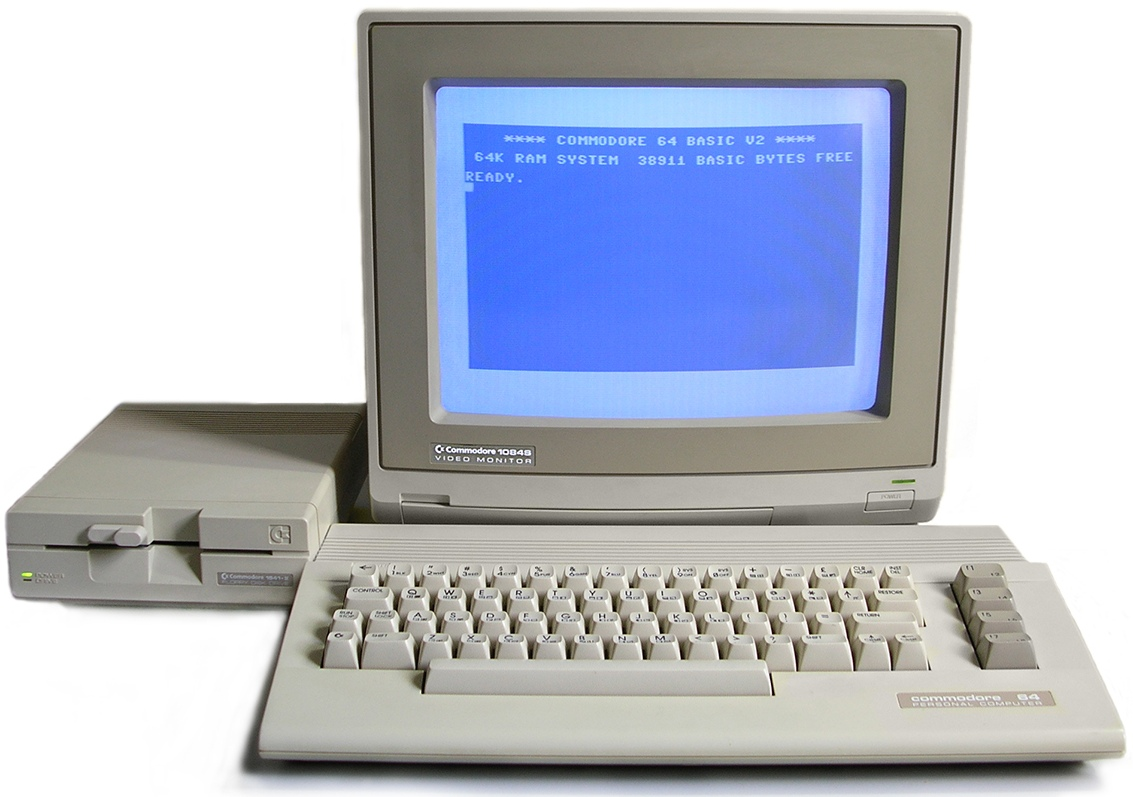
\includegraphics[width=.9\textwidth]{img/c64}
        \end{center}
        \Justified{
            \textbf{Commodore 64:}
            Früher Heimcomputer der 1980er-Jahre
            mit eingebautem BASIC-Interpreter
        }

        \column{.48\textwidth}
        \begin{center}
            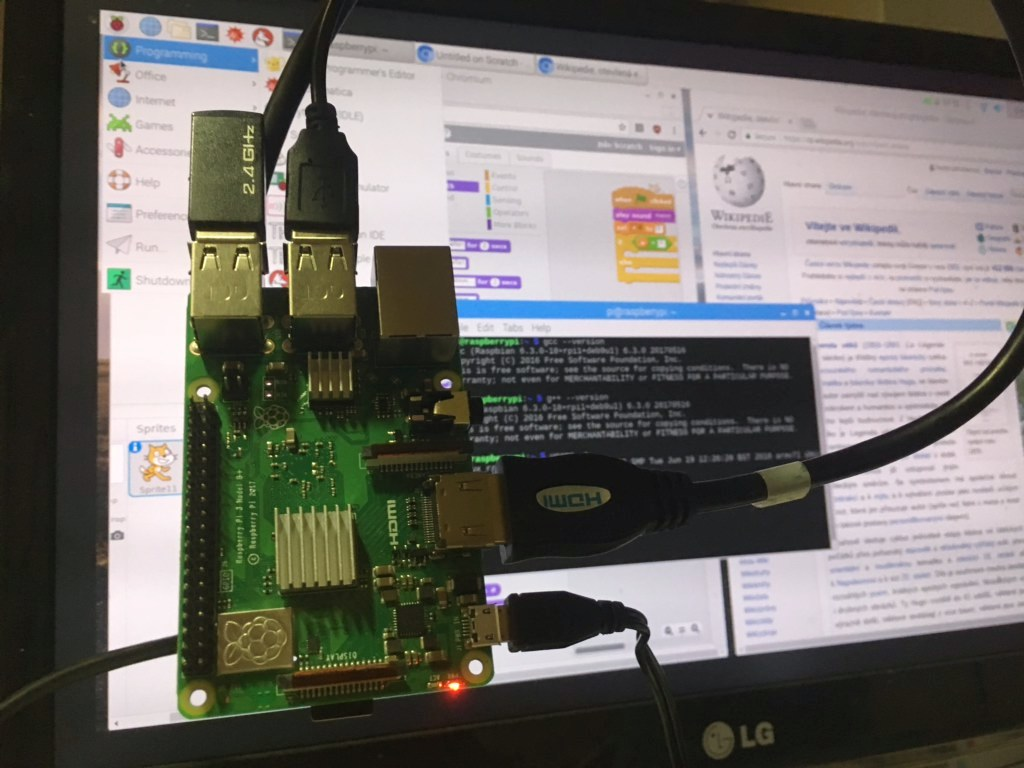
\includegraphics[width=.85\textwidth]{img/raspi}
        \end{center}
        \Justified{
            \textbf{Rasbperry Pi:} Moderner Versuch, einen Computer zum
            Experimentieren und Programmieren Lernen zu bauen
        }
    \end{columns}
\end{frame}
}

%%% Folien
{
\scriptsize
\setlength{\fboxsep}{0pt}

\begin{frame}[allowframebreaks]{Installation des Raspberry Pi OS}
    \begin{center}
        \fbox{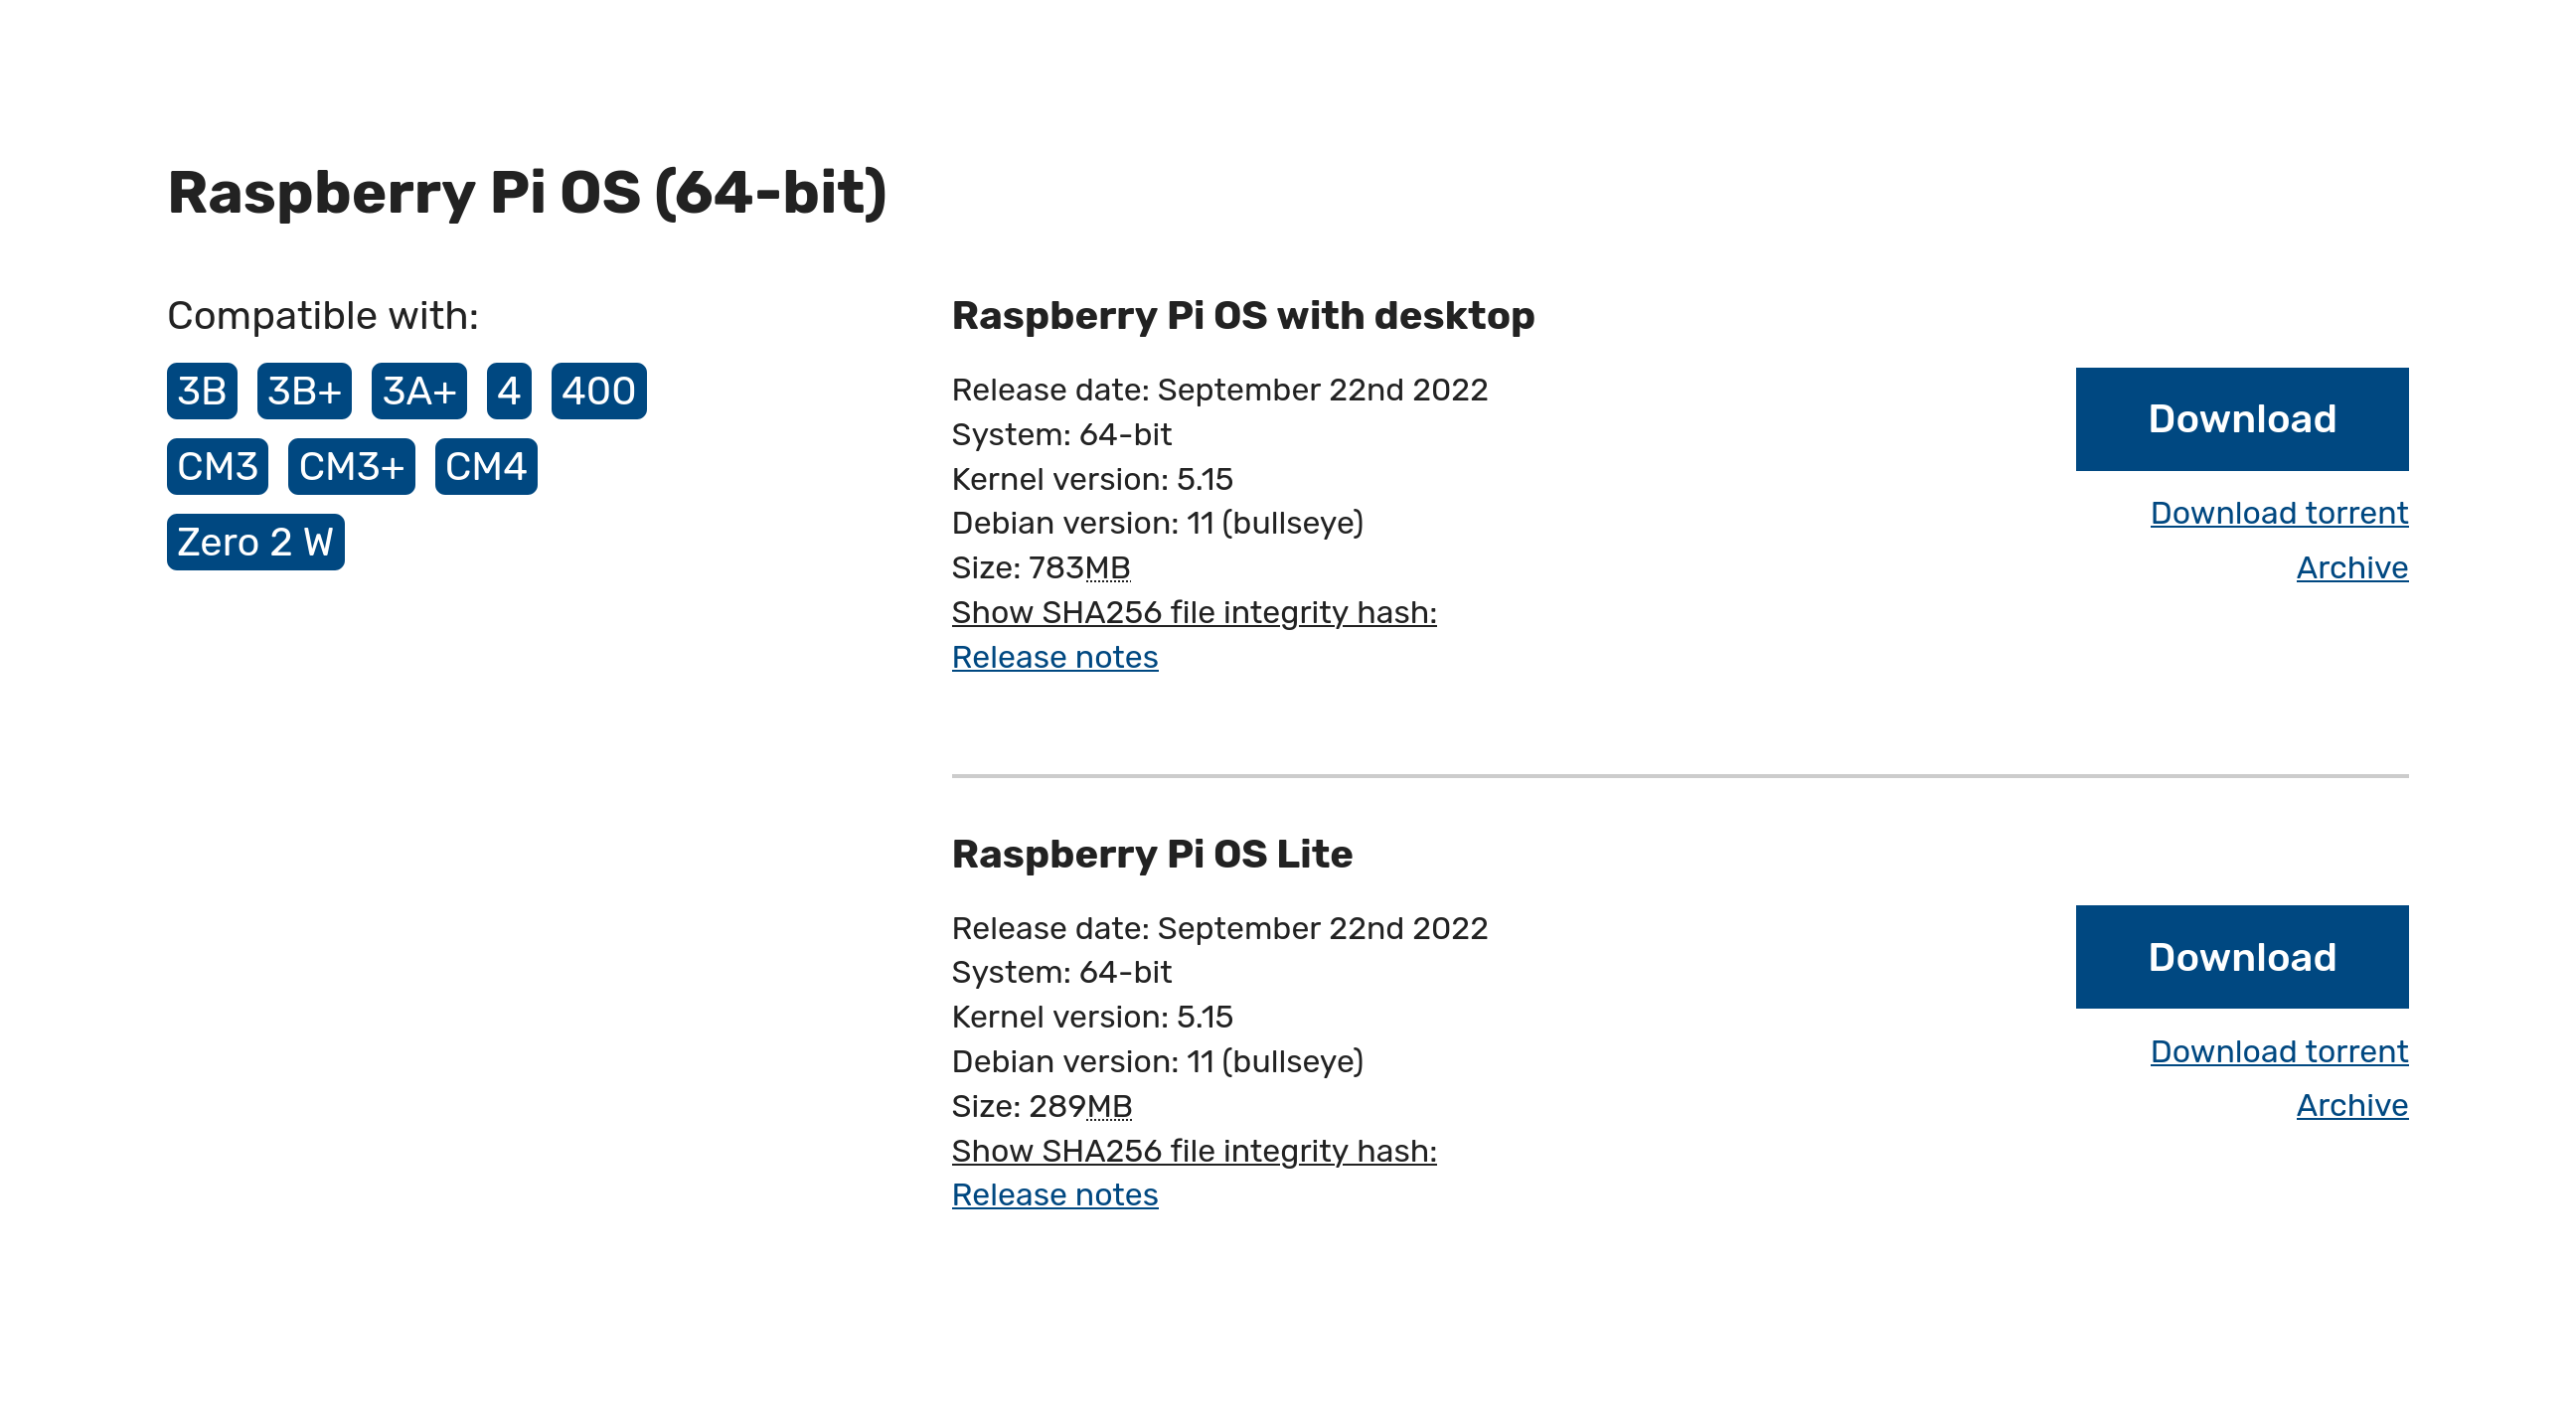
\includegraphics[width=.9\textwidth]{img/raspios-download}}
    \end{center}

    \Justified{
        Das Rasbperry Pi OS (abgeleitet von Raspbian bzw. Debian Linux) wird als Image File
        auf der offiziellen Webseite der Rasbperry Pi Foundation zum Download angeboten.
        Für eingebettete Anwendungen sollte bevorzugt die Lite-Variante ohne Desktopumgebung
        und Anwendungssoftware verwendet werden. Mit entsprechendem Expertenwissen kann man
        natürlich auch sein eigenes Linux-System bauen, zum Beispiel mit Buildroot. \smiley{}
    }

    \smallskip
    \LinkButton{https://www.raspberrypi.com/software/operating-systems/}{Downloadseite des Raspberry Pi OS}
    \LinkButton{https://www.wpvs.de/repo/iot-workshop/05-Werkzeuge/Erste\%20Schritte\%20mit\%20Linux,\%20Buildroot\%20und\%20Debootstrap.pdf}{Anleitung zum Selberbauen}

    %%%
    \framebreak

    \begin{center}
        \fbox{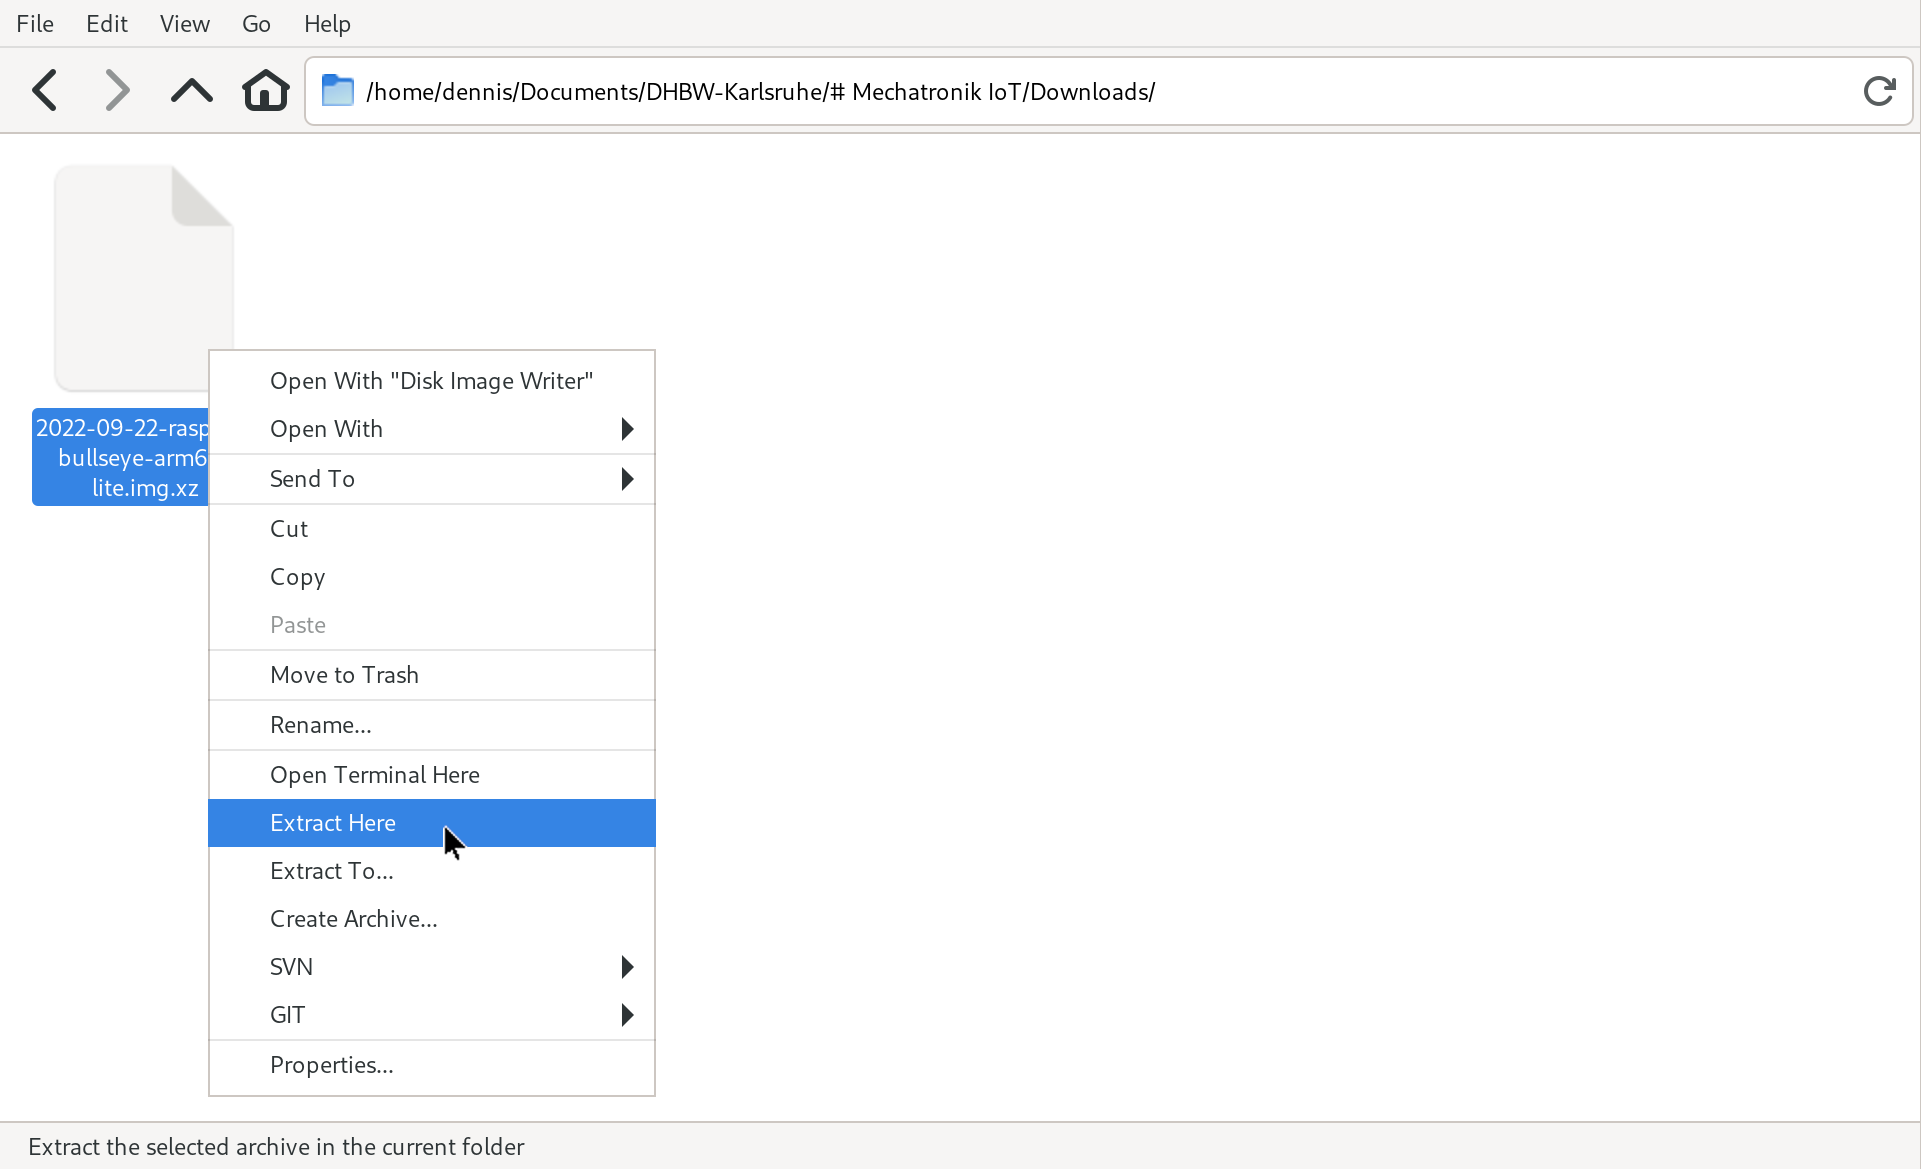
\includegraphics[width=.9\textwidth]{img/raspios-entpacken}}
    \end{center}

    \Justified{
        Um die Downloadgröße klein zu halten, ist die Abbilddatei komprimiert. Sie muss daher mit
        einem geeigneten Programm zunächst entpackt werden, wenn das Programm zum Schreiben der
        SD-Karte dies nicht automatisch macht.
    }

    %%%
    \framebreak

    \begin{center}
        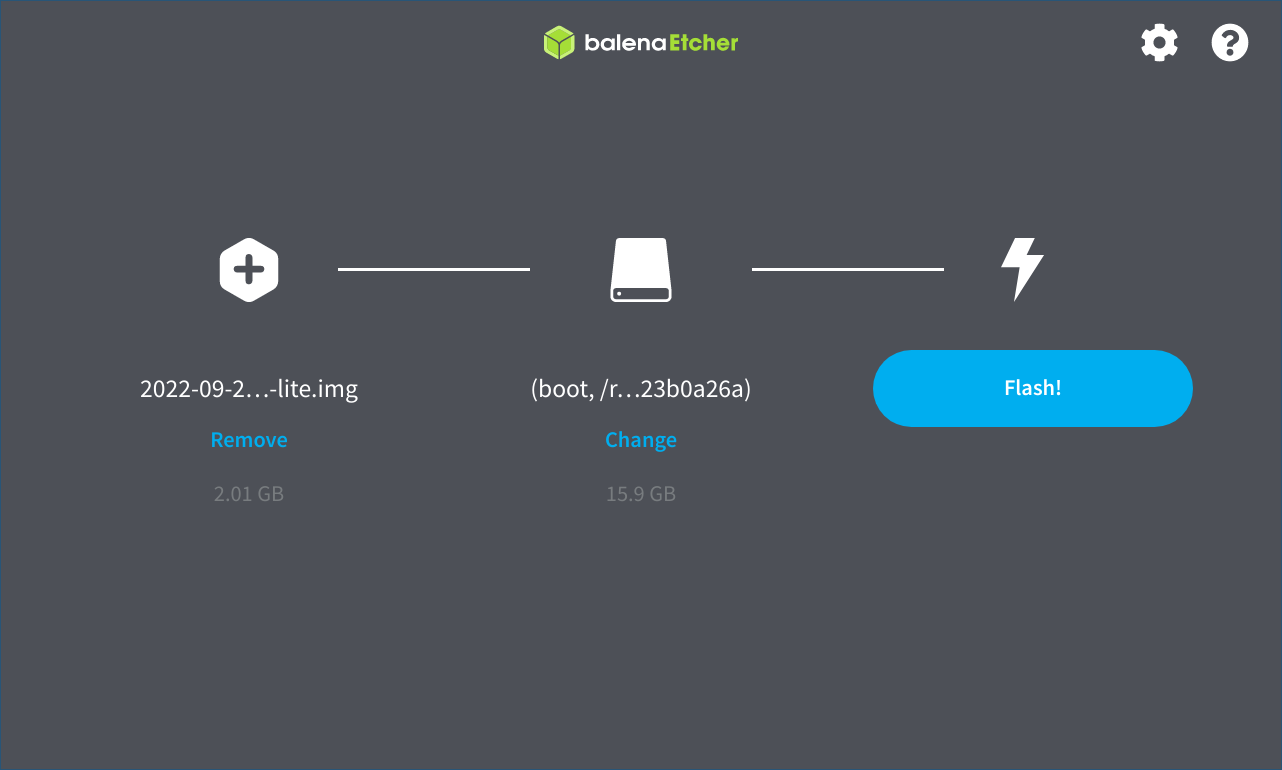
\includegraphics[width=.75\textwidth]{img/raspios-flash}
    \end{center}

    \Justified{
        Anschließend kann die Datei mit einem geeigneten Programm auf eine SD-Karte geschrieben werden.
        Wichtig ist, dass \textcolor{RoyalPurple}{der Inhalt der Datei bitweise} übertragen wird.
        Hierfür kann zum Beispiel der Balena Etcher, der für alle gängigen Betriebssysteme zur Verfügung
        steht, verwendet werden. Ein einfaches Kopieren der Datei mit dem Explorer wird hingegen nicht
        funktionieren.
    }

    \smallskip
    \LinkButton{https://www.balena.io/etcher/}{Downloadseite des Balena Etcher}

    %%%
    \framebreak

    \begin{center}
        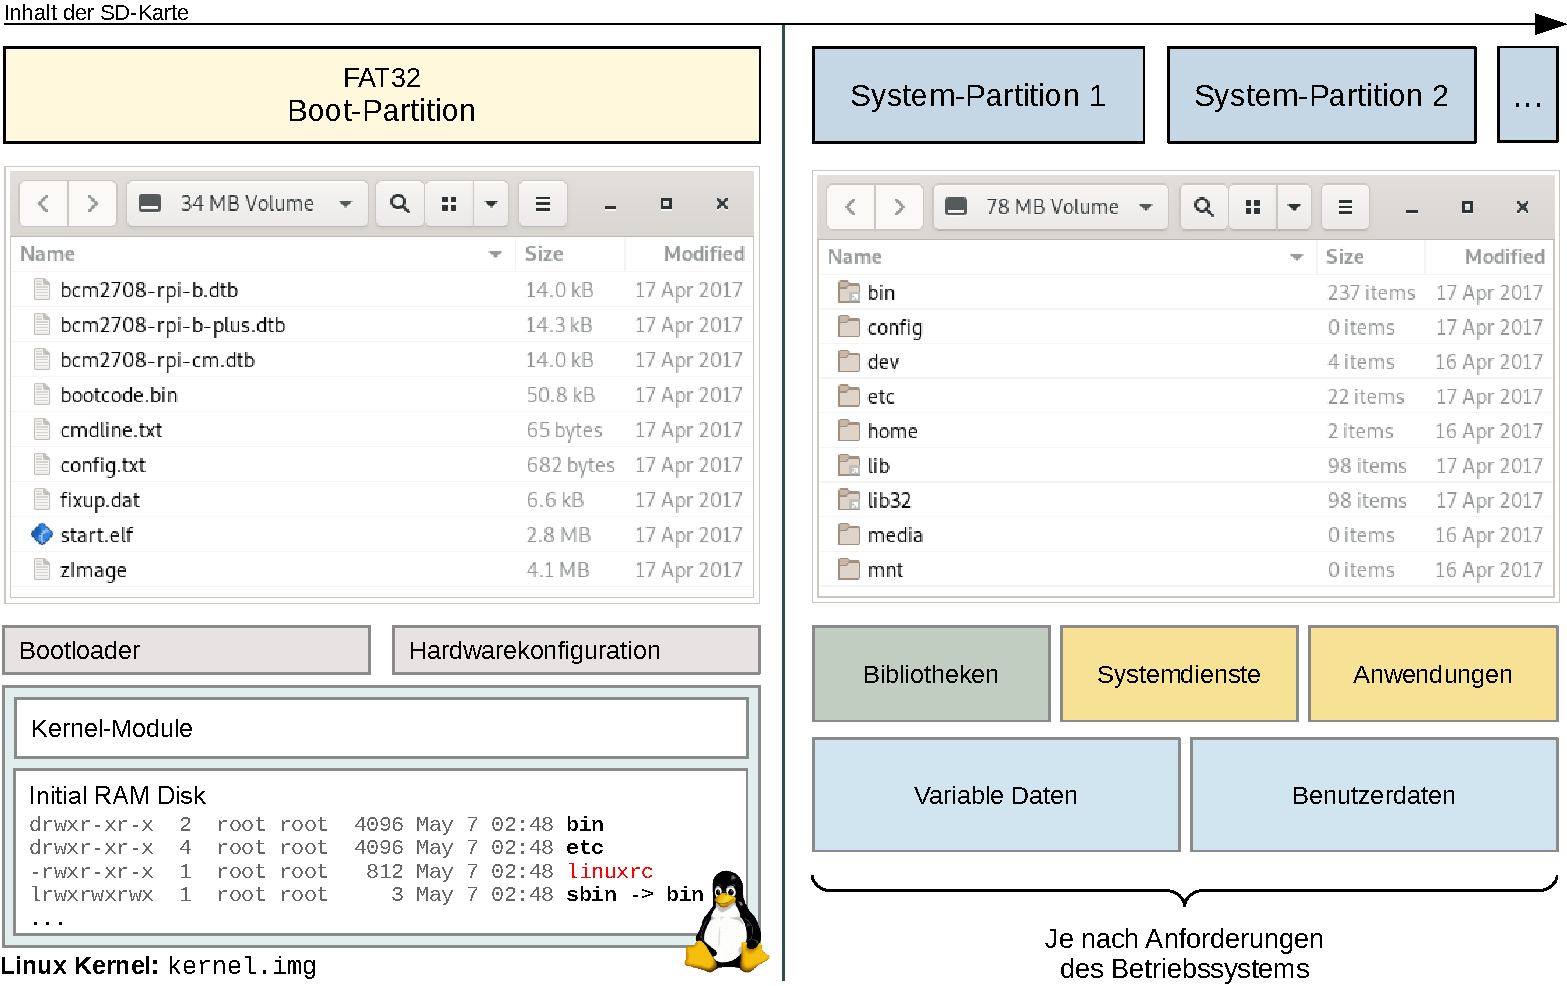
\includegraphics[width=.9\textwidth]{img/raspios-partitionen}
    \end{center}

    \Justified{
        Im Ergebnis sollten mindestens zwei Partitionen auf der SD-Karte vorhanden sein, wobei unter
        Windows nur die Boot-Partition angezeigt wird. Vom Linux-Kernel abgesehen liegen das eigentliche
        Betriebssystem sowie alle Anwendungsdaten in der zweiten Partition.
    }
\end{frame}
}

%%% Folie
\begin{frame}{Der Bootvorgang des Raspberry Pi im Detail}
    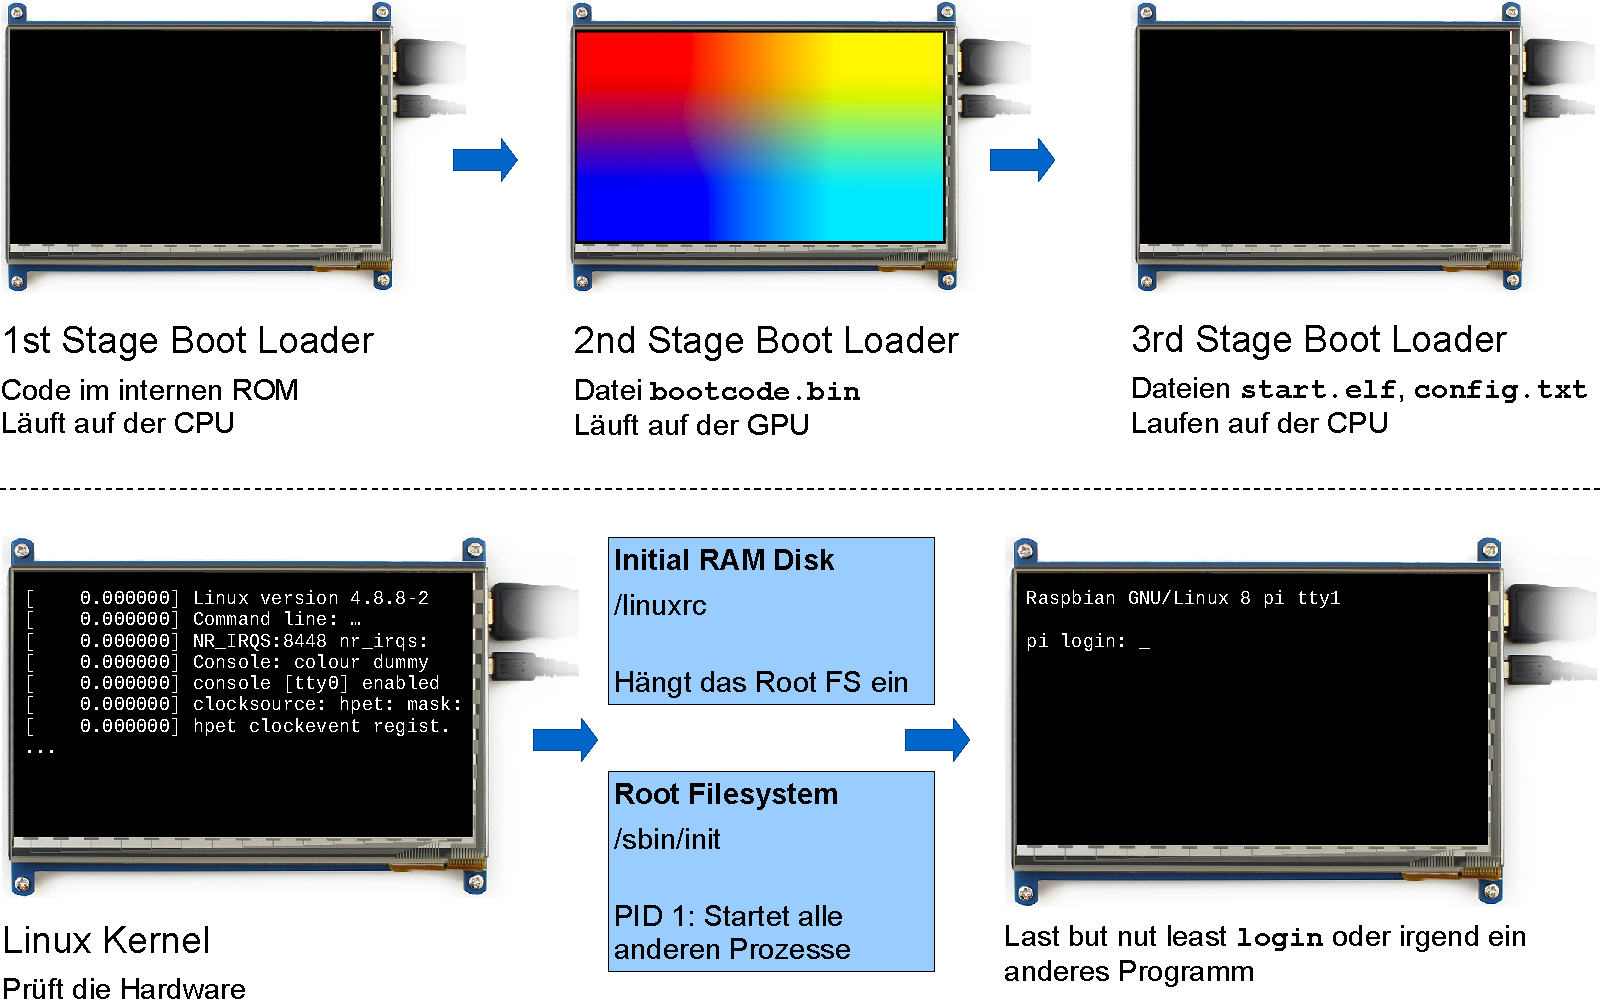
\includegraphics[width=\textwidth]{img/pi-bootvorgang}
\end{frame}

%%% Folien
{
\scriptsize
\setlength{\fboxsep}{0pt}

\begin{frame}[allowframebreaks]{Abschluss der Installation}
    \begin{center}
        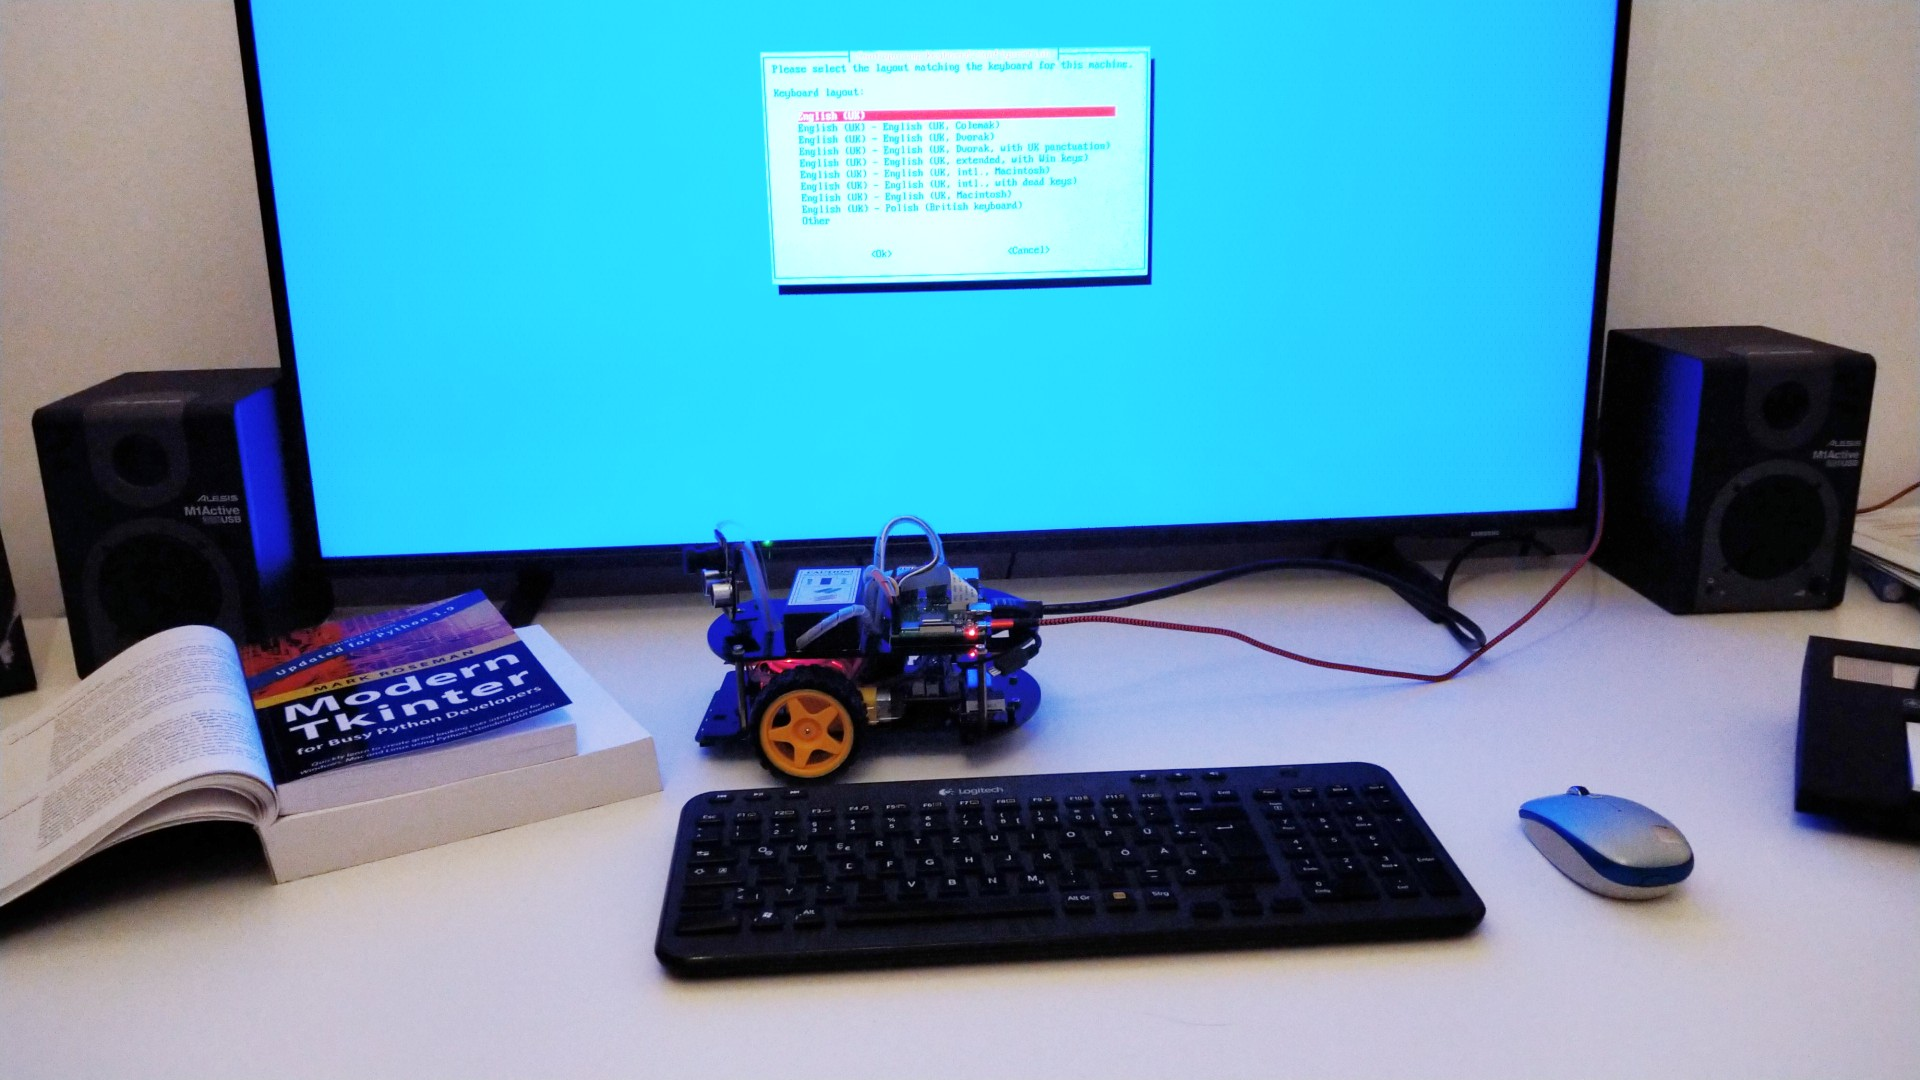
\includegraphics[width=.9\textwidth]{img/raspios-erststart}
    \end{center}

    \Justified{
        Die nächsten Schritte erfolgen auf dem Raspberry Pi. Hierfür müssen zumindest einmal
        Bildschirm, Tastatur und Maus verbunden werden. Anschließend die SD-Karte einlegen und das
        USB-Stromkabel einstecken. Nach einer Weile sollte das System neustarten und ein Menü zum
        Abschluss der Installtion zeigen.
    }

    %%%
    \framebreak

    \begin{center}
        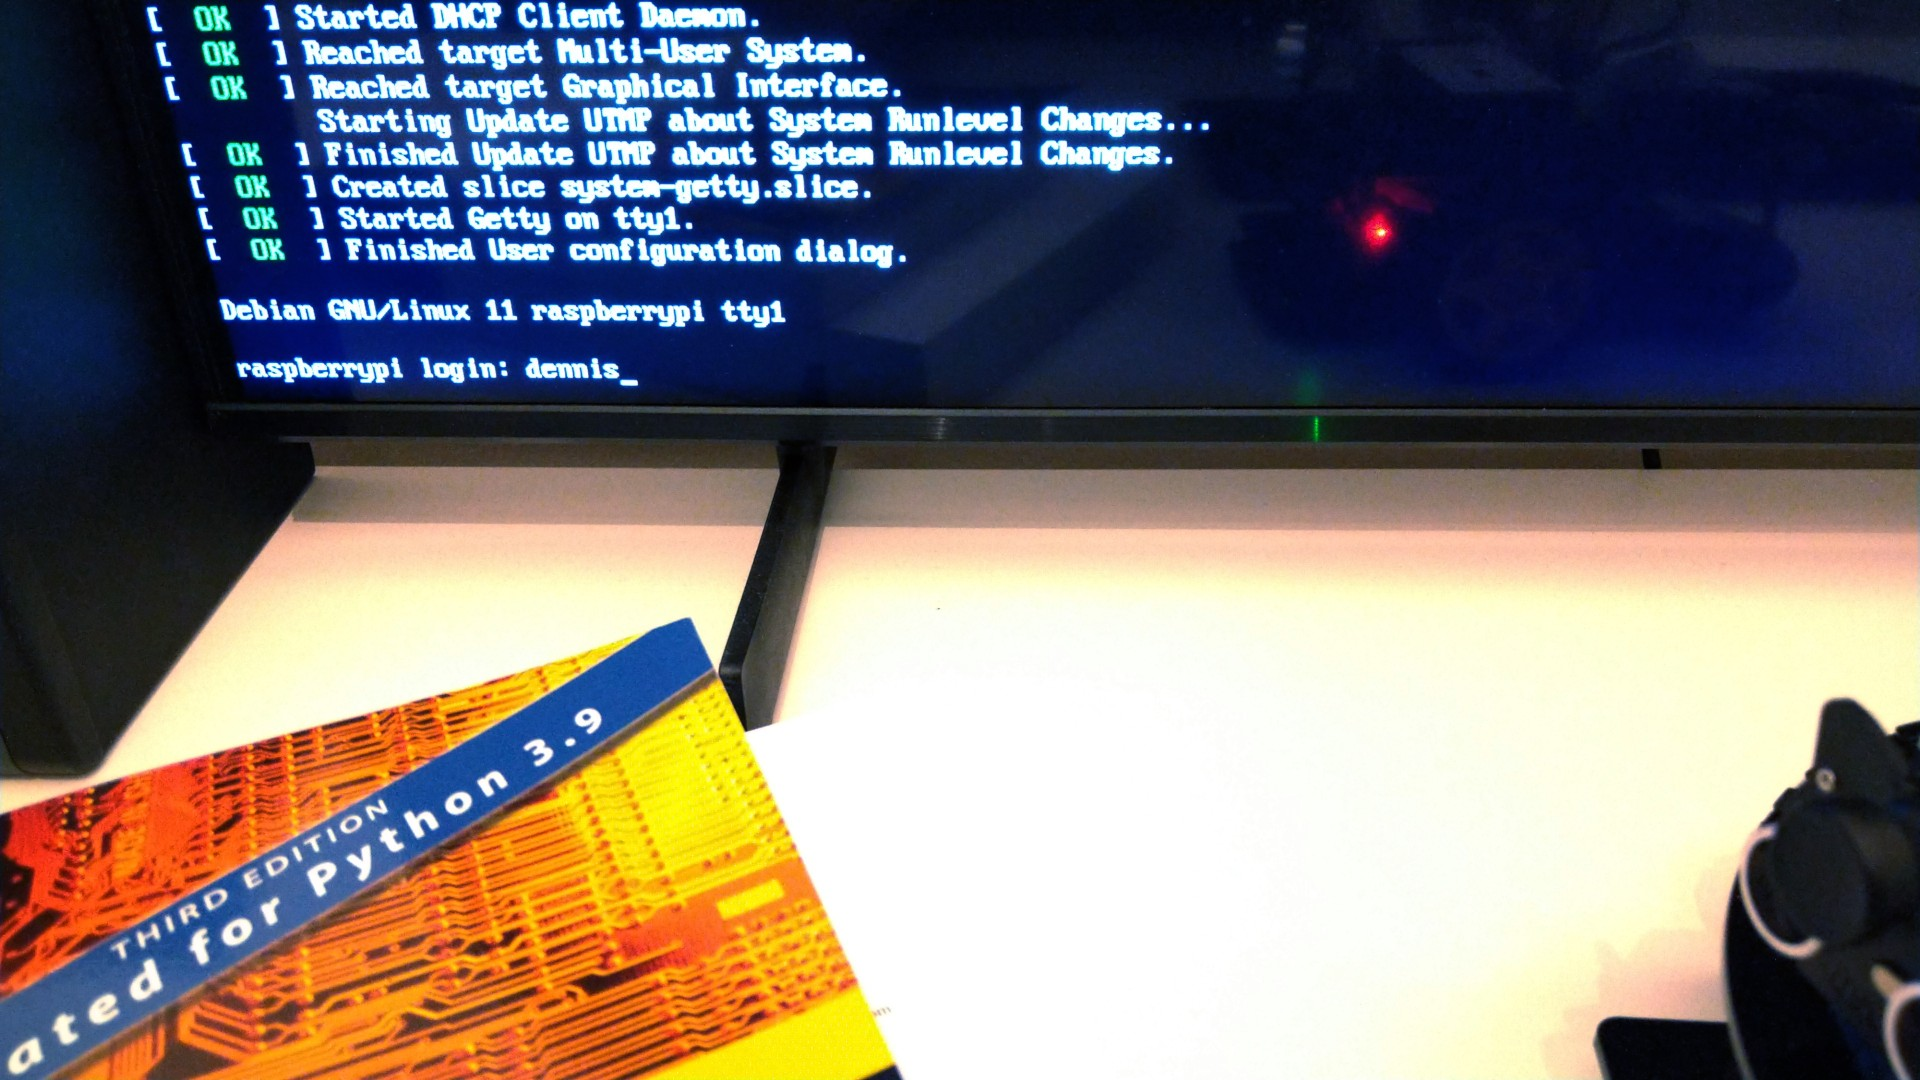
\includegraphics[height=14em]{img/raspios-login}
        \hfill
        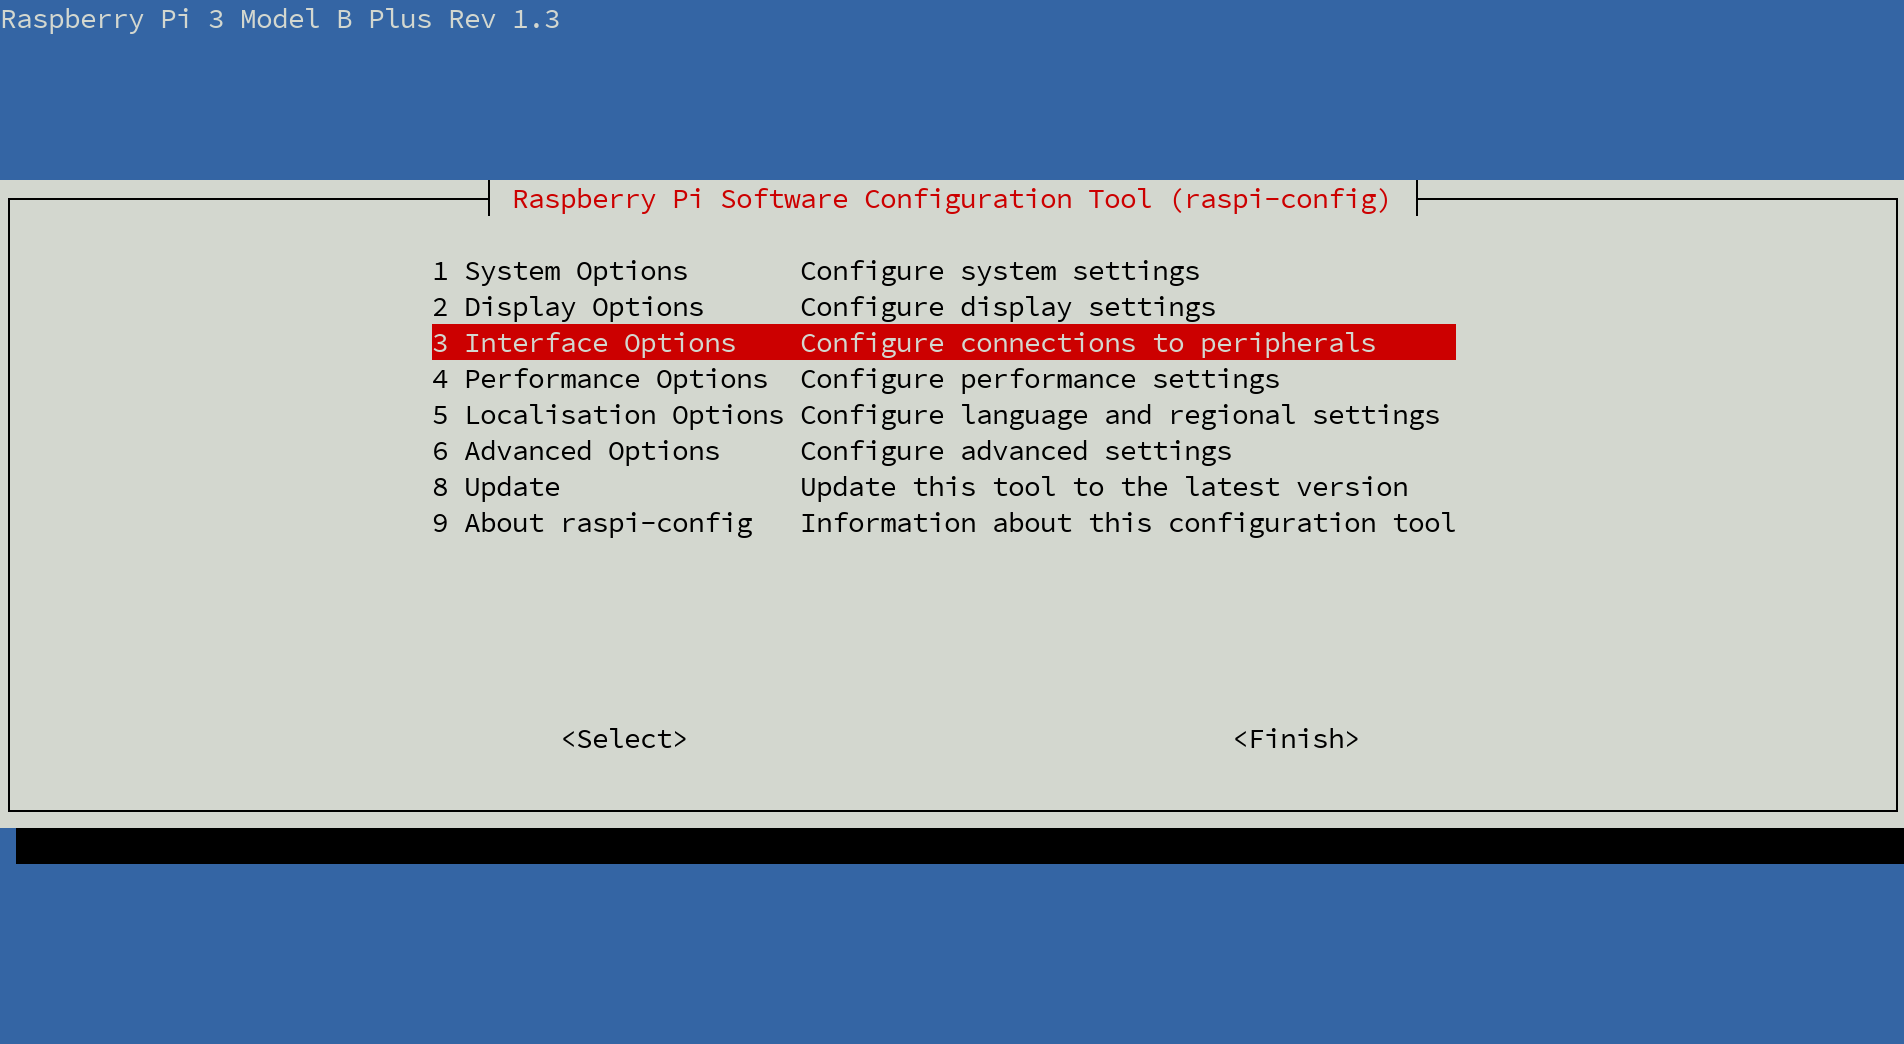
\includegraphics[height=14em]{img/raspi-config-1}
    \end{center}

    %~ \begin{center}
        %~ 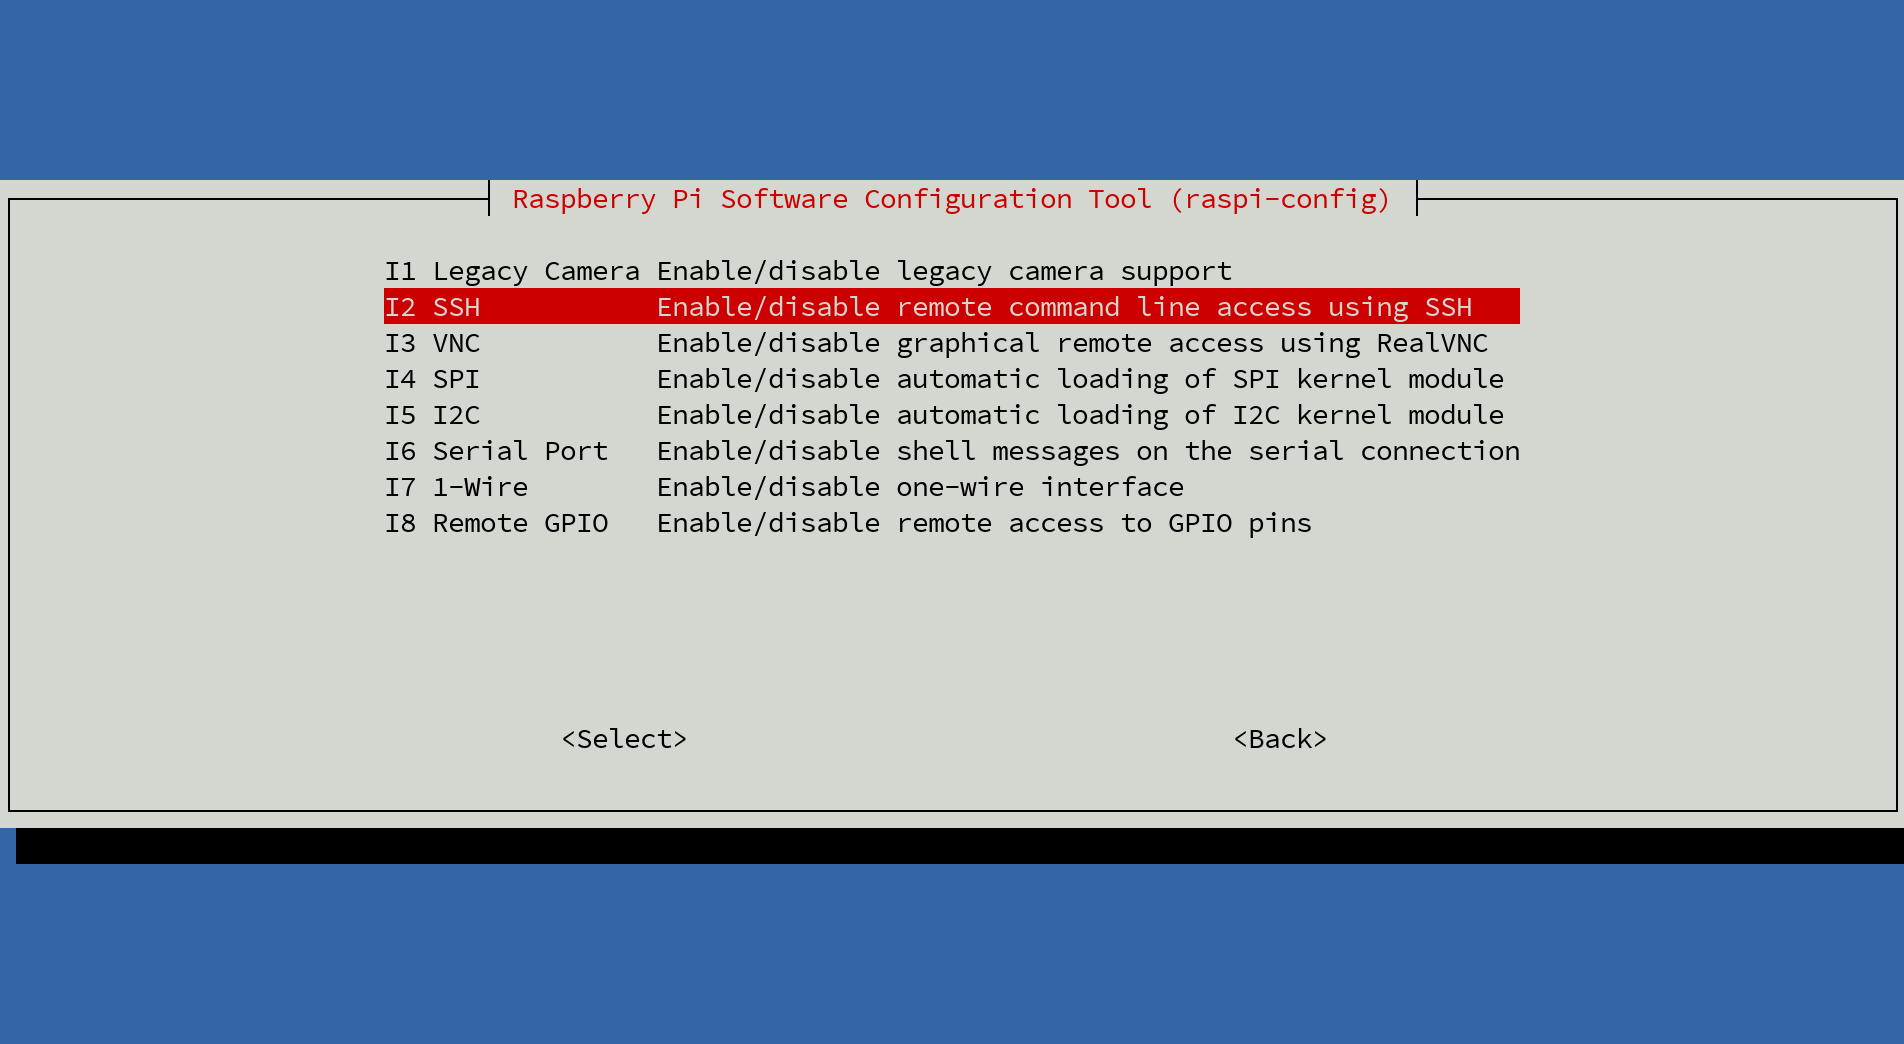
\includegraphics[height=14em]{img/raspi-config-2}
        %~ \hfill
        %~ 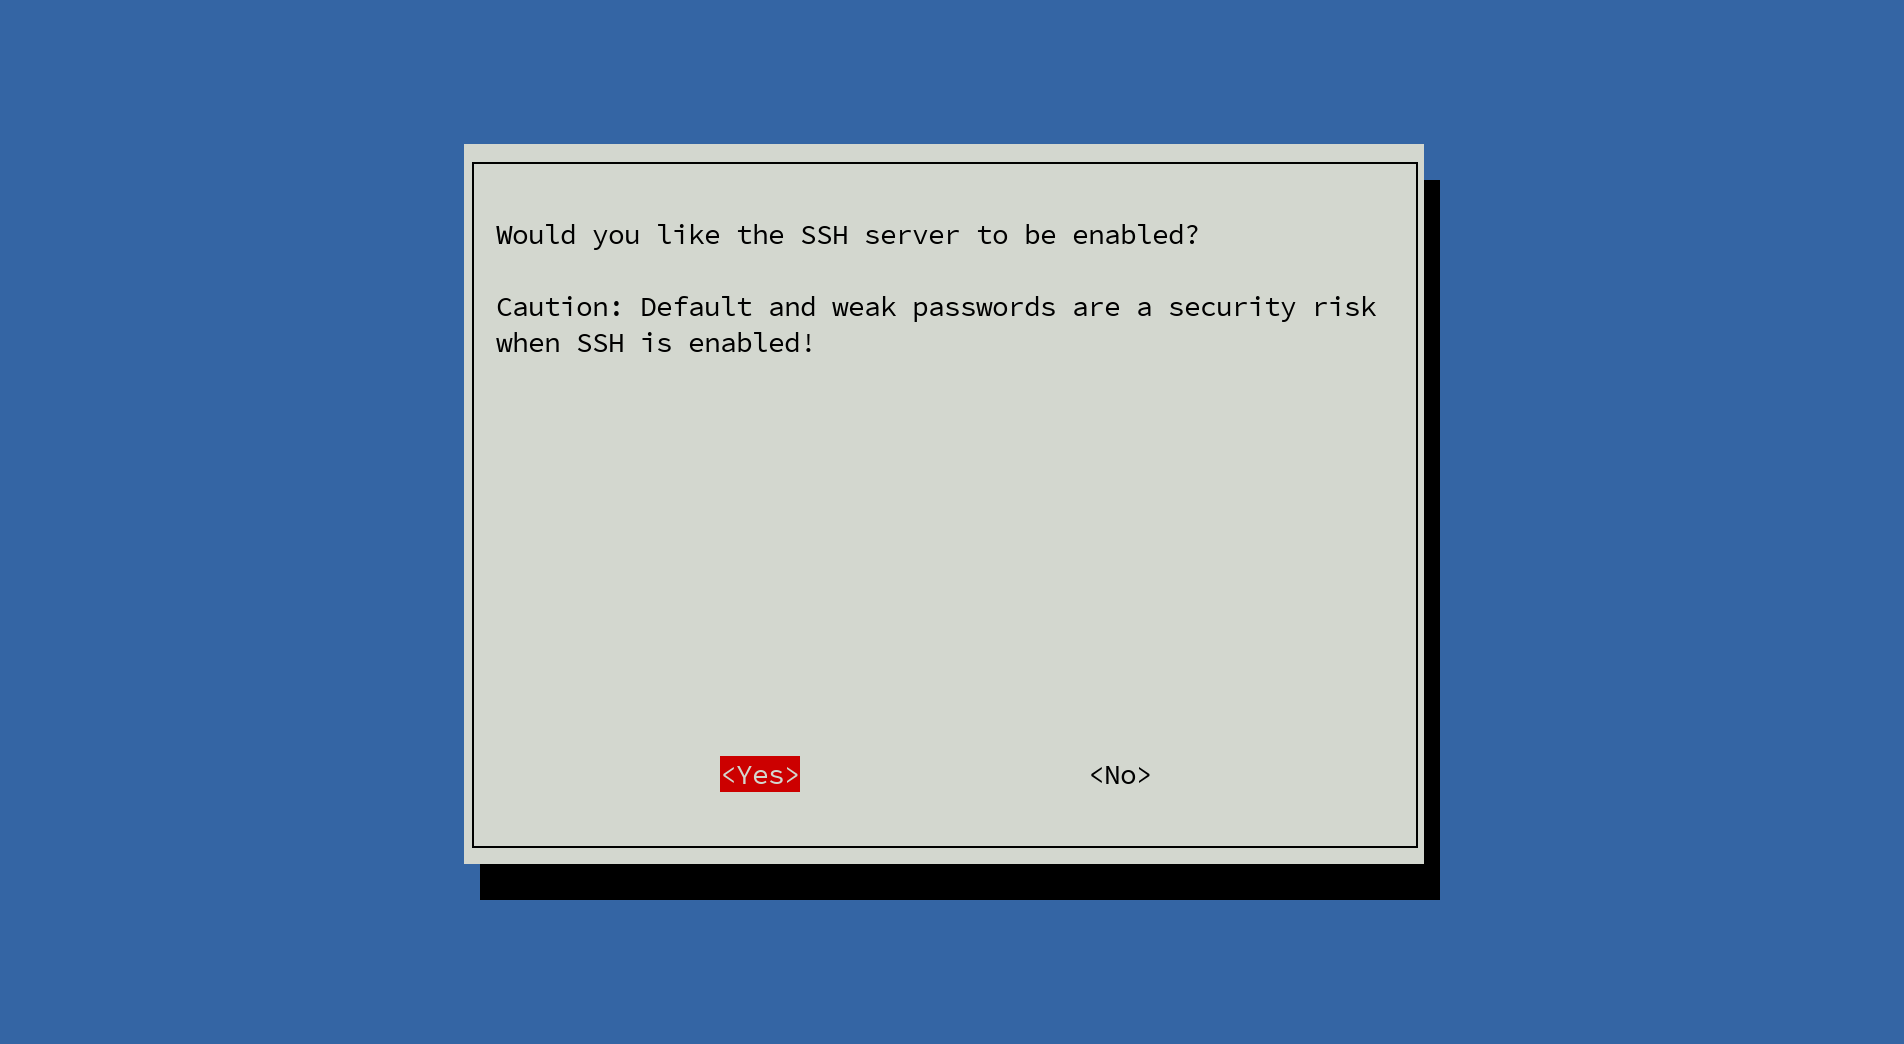
\includegraphics[height=14em]{img/raspi-config-3}
    %~ \end{center}

    \Justified{
        \smallskip
        Kurz darauf erscheint der Login-Prompt. Dort Benutzernamen und Passwort eingeben, um sich
        anzumelden und dann den Befehl \texttt{sudo raspi-config} ausführen. Es handelt sich dabei
        um ein einfaches Konfigurationswerkzeug für das Raspberry Pi OS. Folgende Einstellungen sind
        dort für uns relevant:
        \smallskip
    }

    \begin{itemize}
        \item System Options $\rightarrow$ Wireless LAN $\rightarrow$ \textit{Name und Passwort des WLANs}
        \item Interface Options $\rightarrow$ SSH $\rightarrow$ \textit{aktivieren}
        \item Interface Options $\rightarrow$ SPI $\rightarrow$ \textit{aktivieren}
        \item Interface Options $\rightarrow$ I2C $\rightarrow$ \textit{aktivieren}
        \item Interface Options $\rightarrow$ 1-Wire $\rightarrow$ \textit{aktivieren}
    \end{itemize}

    \Justified{
        \smallskip
        Anschließend muss der Raspberry Pi neugestartet werden, um die Änderungen wirksam werden zu lassen.
    }

    %%%
    \framebreak

    \begin{center}
        \fbox{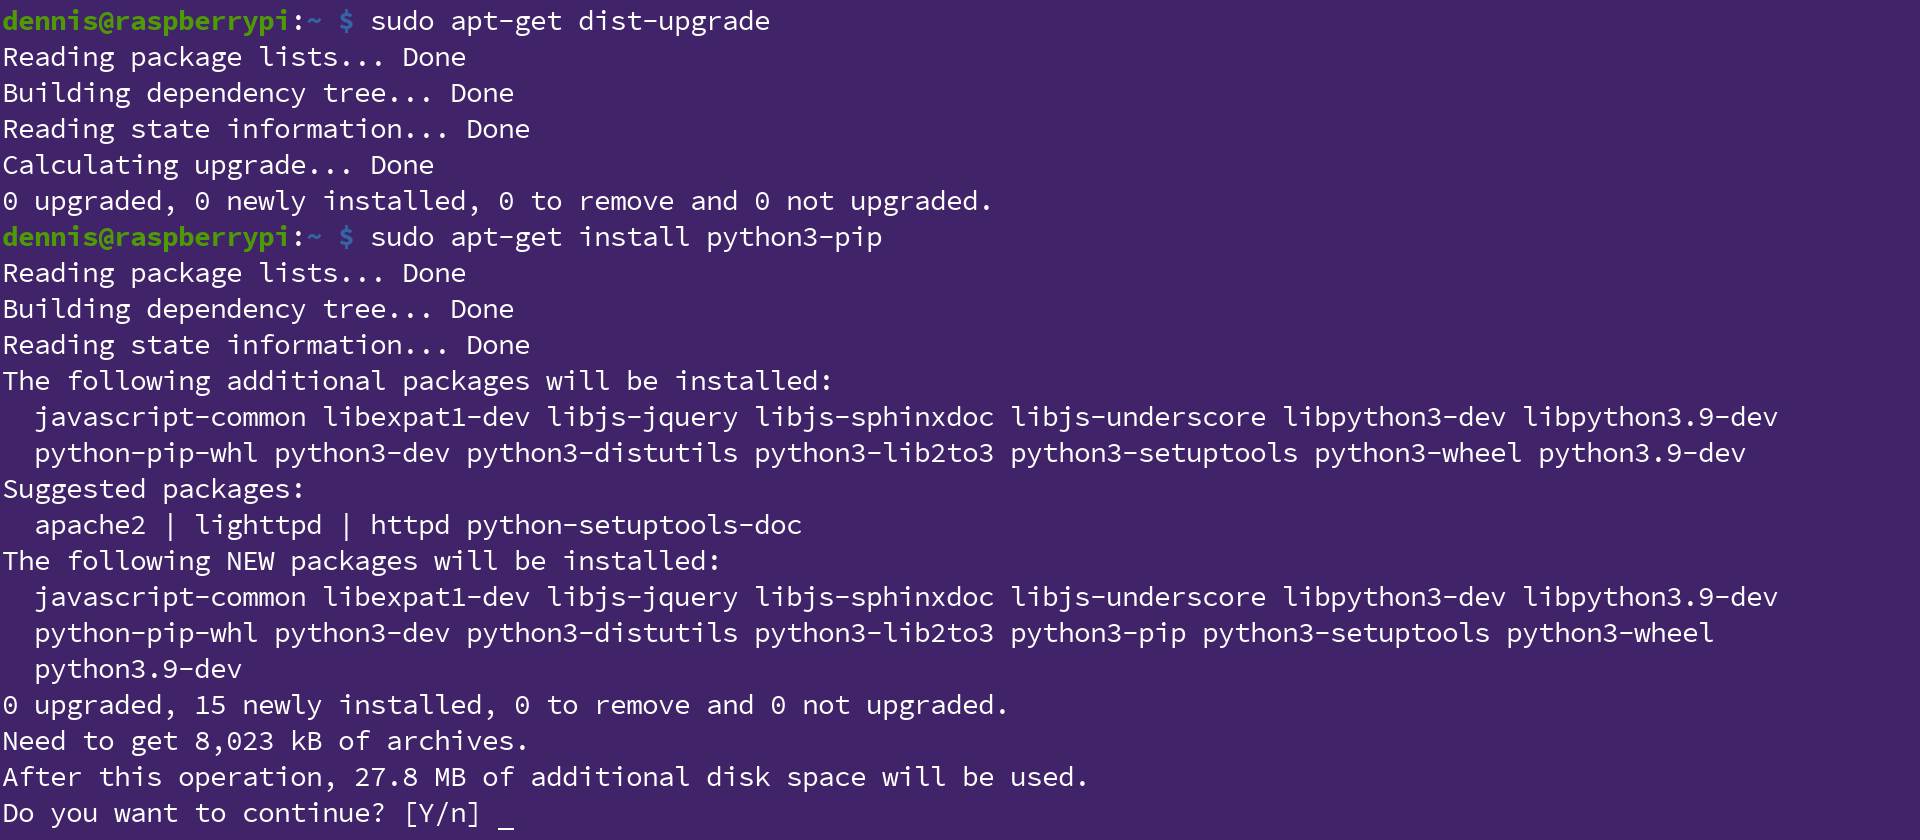
\includegraphics[width=\textwidth]{img/raspios-apt}}
    \end{center}

    \Justified{
        Zum Schluss führen Sie noch folgende Befehle aus, um eventuell vorhandene Update einzuspielen,
        sowie zusätzliche Programme zu installieren:
        \smallskip

        \texttt{sudo apt dist-upgrade} \\
        \texttt{sudo apt install python3-pip python3-venv git golang}
    }
\end{frame}
}

%%% Folie
\begin{frame}{Der Alltag mit Linux \smiley{}}
    \begin{center}
        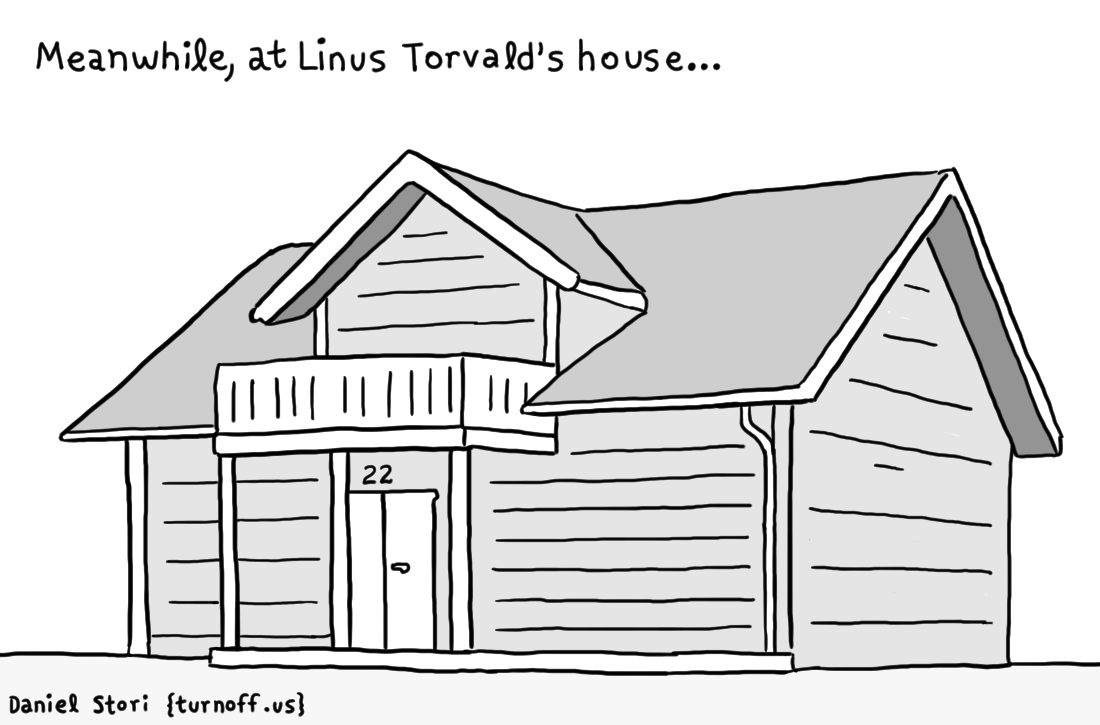
\includegraphics[width=.7\textwidth]{img/linus-torvalds-house}
    \end{center}

    \smallskip

    \begin{center}
        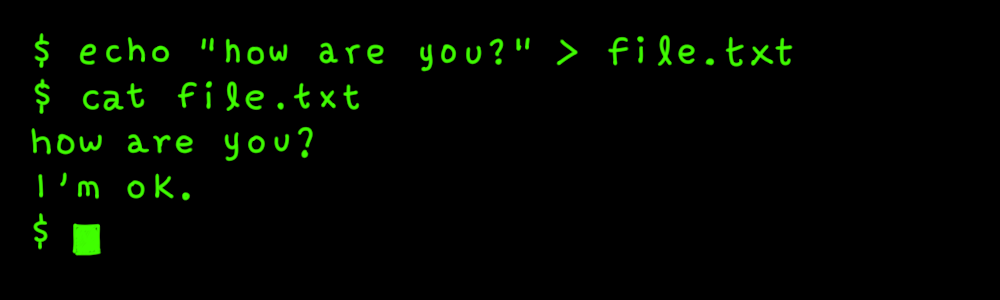
\includegraphics[width=.7\textwidth]{img/ghost-in-the-shell}
    \end{center}
\end{frame}

%%% Folie
{
\scriptsize
\setlength{\leftmargini}{1.2em}

\begin{frame}{Kernel vs. Userland}
    \Justified{
        Linux-basierte Betriebssysteme setzen sich immer aus dem \textbf{Kernel}
        und dem \textbf{Userland} zusammen. Der Kernel beinhaltet dabei lediglich
        die Grundfunktionen für Hardwarezugriffe, Multitasking, Speicherverwaltung
        usw. Alle anderen Teile des Betriebssystems sind Bestandteil des Userlands
        und können somit stark variieren.
    }

    {
        \tiny

        \begin{columns}[T,onlytextwidth]
            \column{.49\textwidth}
            \begin{itemize}
                \justifying

                \item \textbf{Bibliotheken:} Von den installierten Programmen
                benötigte Quellcode-Bibliotheken mit gemeinsamen Funktionen.
                Zum Beispiel \texttt{libc} oder \texttt{libgtk}.

                \item \textbf{Systemdienste:} Hintergrundjobs und Hilfsprogramme des
                Betriebssystems. Zum Beispiel NTP-Daemon, Druckerspooler oder die
                Shell bzw. grafische Desktopumgebung.

                \item \textbf{Anwendungen:} Nicht direkt zum Betriebssystem gehörende,
                jedoch zur Nutzung durch die Anwender*innen vorgesehene Programme, wie
                zum Beispiel Webbrowser oder Media Player.
            \end{itemize}

            \column{.49\textwidth}
            \begin{itemize}
                \justifying

                \item \textbf{Variable Daten:} Während dem regulären Systembetrieb
                anfallende Verwaltungsdaten, wie Systemprotokolle, temporäre Dateien
                oder zwischengespeicherte Druckaufträge.

                \item \textbf{Benutzerdaten:} In der Hoheit der Benutzer*innen liegende
                Dateien, wie zum Beispiel Bilder oder Dokumente.
            \end{itemize}
        \end{columns}
    }

    \bigskip
    $\Rightarrow$ \textbf{GNU/Linux:} Linux-Kernel mit GNU-Userland (plus weiteren Bestandteilen) \\
    $\Rightarrow$ \textbf{Android:} Linux-Kernel mit nahezu komplett in Java entwickeltem Userland

    \vfill
    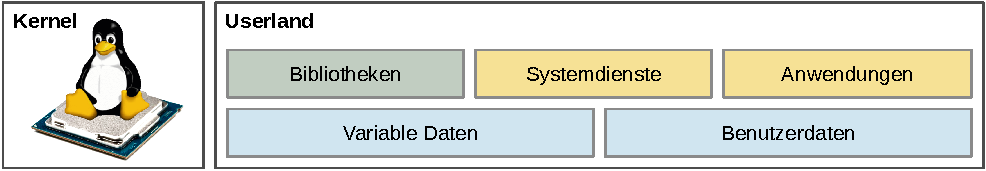
\includegraphics[width=\textwidth]{img/linux-bestandteile}
\end{frame}
}

%%% Folie
{
\scriptsize

\begin{frame}[allowframebreaks]{Der Linux Filesystem Hierarchy Standard}
    \begin{center}
        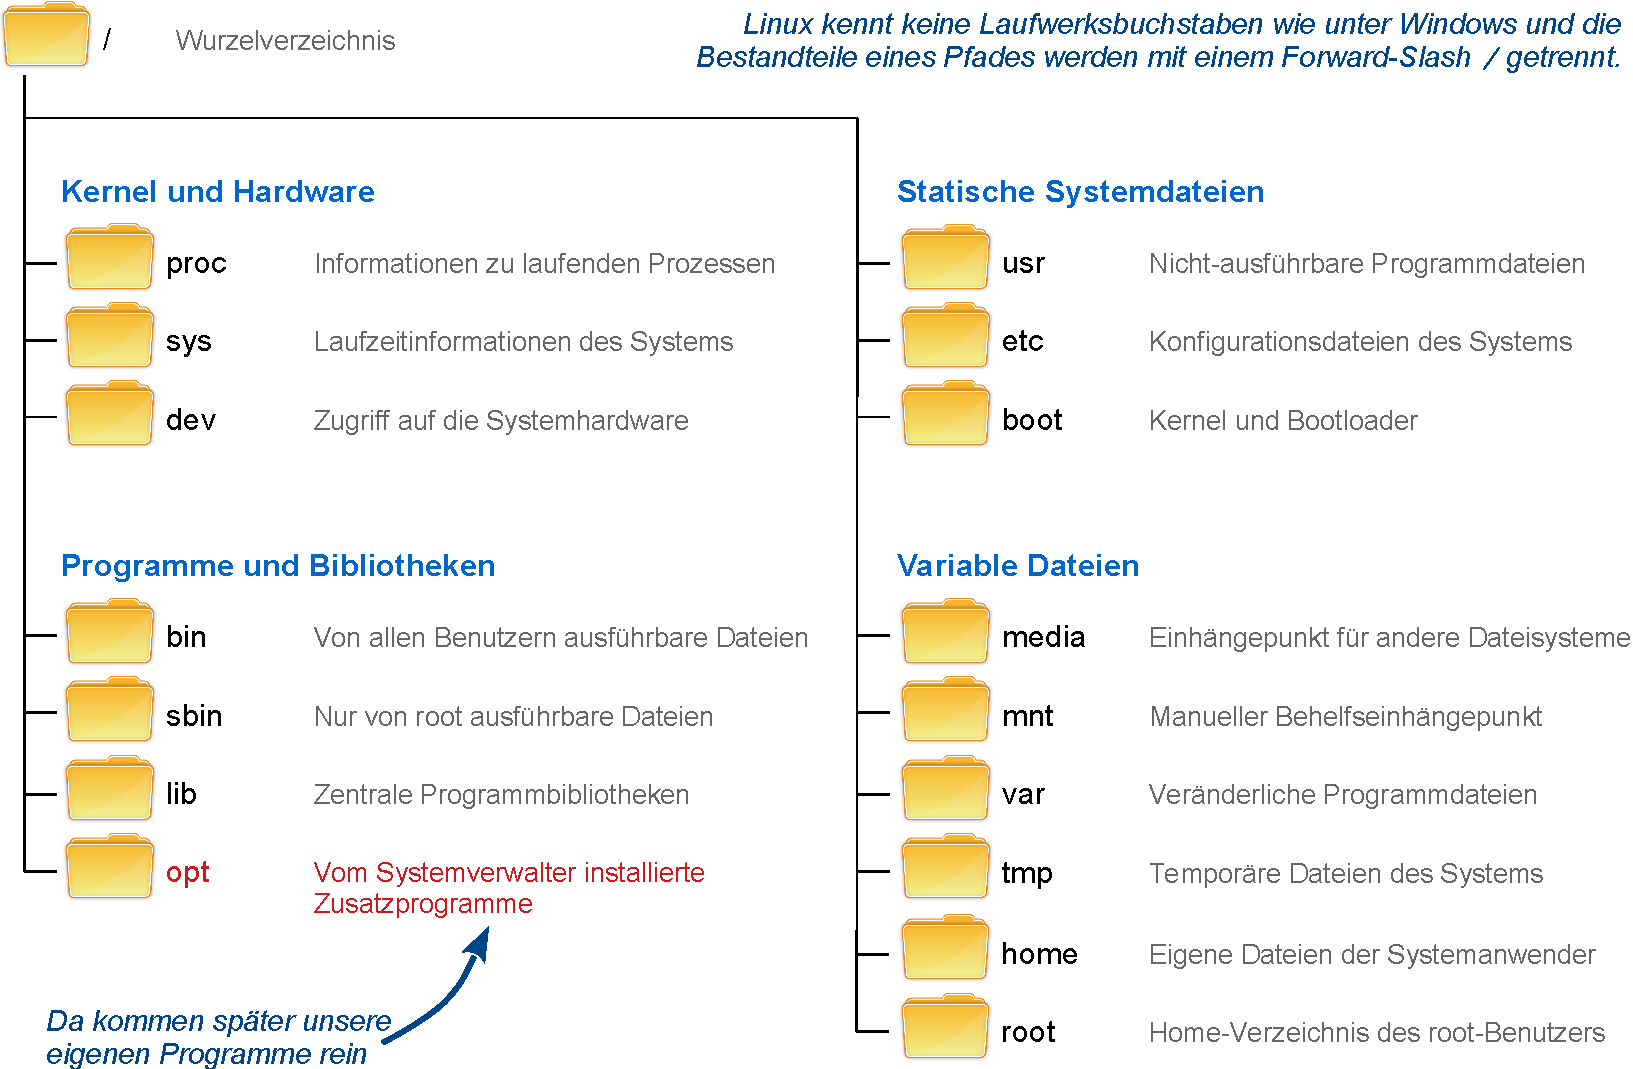
\includegraphics[width=\textwidth]{img/fhs-verzeichnisse}
    \end{center}

    \framebreak

    \begin{columns}[T]
        \column{.8\textwidth}
        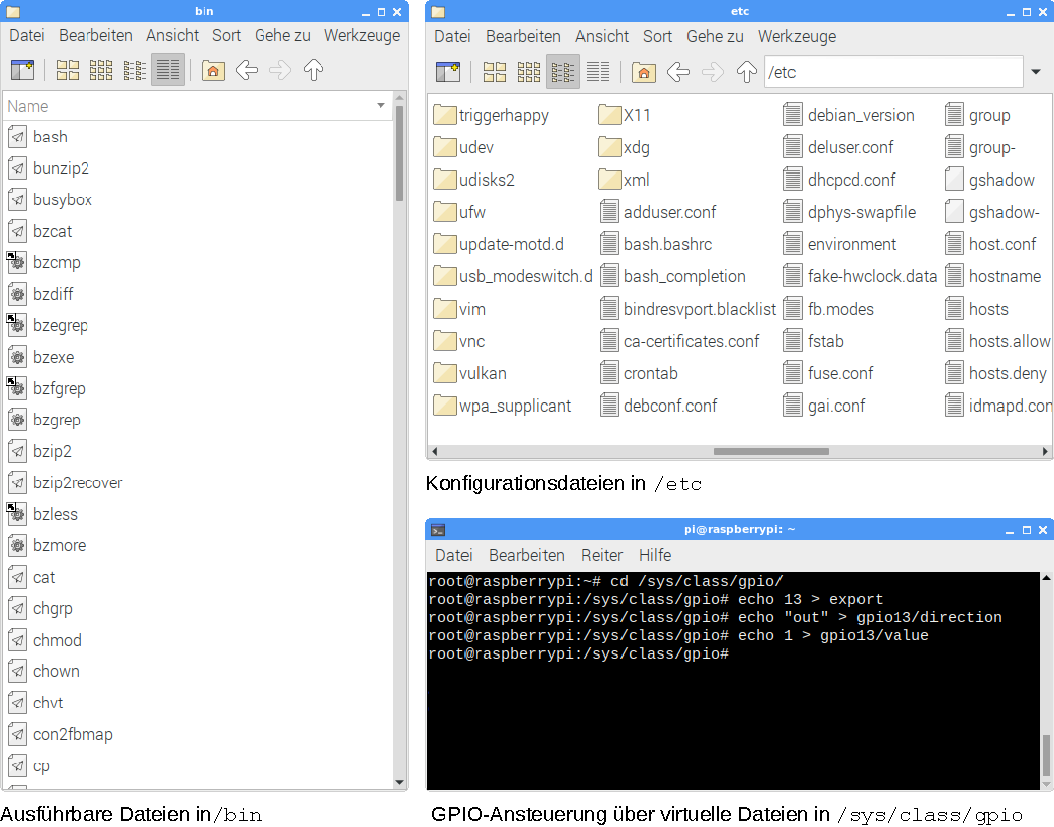
\includegraphics[width=\textwidth]{img/fhs-beispiele}

        \column{.3\textwidth}
        \Justified{
            Aufgrund der konzeptionellen Nähe zu Unix ist unter Linux fast alles
            eine Datei.
            \smallskip

            Die Konfiguration des Systems erfolgt deshalb genau so
            durch Editieren von Konfigurationsdateien, wie der Zugriff auf einen
            Hardwarebaustein nicht viel mehr als das Lesen und Schreiben virtueller
            Dateien erfordert.
        }
    \end{columns}
\end{frame}
}

%%% Folie
{
\scriptsize

\begin{frame}[allowframebreaks]{Fallbeispiel: Systembenutzer unter Linux}
    \begin{center}
        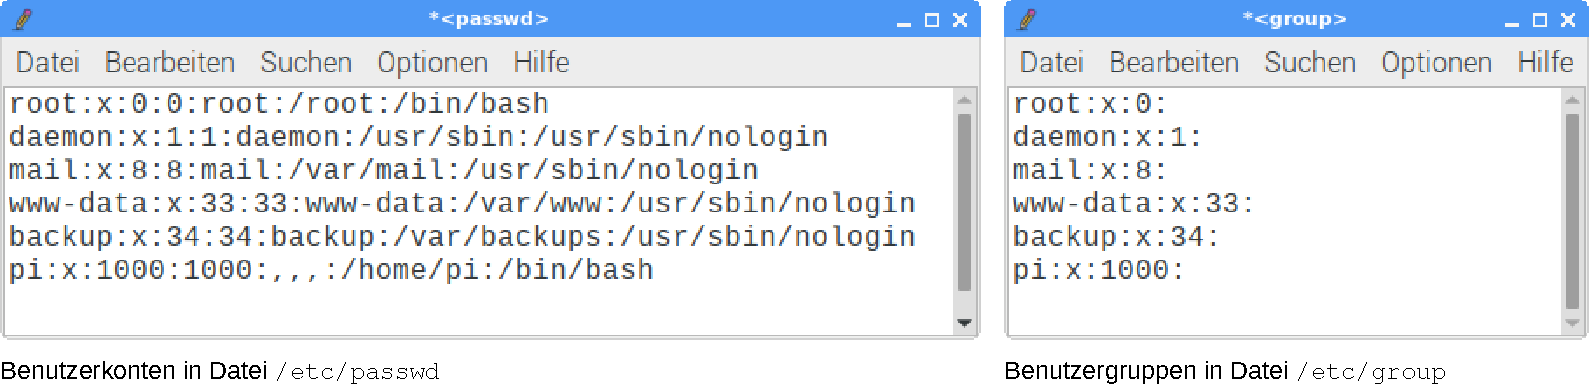
\includegraphics[width=\textwidth]{img/rechte-konfiguration}
    \end{center}

    \Justified{
        Die Benutzerkonten und Benutzergruppen sind in den Dateien
        \texttt{/etc/passwd} und \texttt{/etc/group} definiert. Jeder
        Benutzer bzw. jede Benutzergruppe bekommt hier eine numerische ID
        zugewiesen, die sehr oft nach folgendem Schema vergeben wird:
    }

    \medskip

    {
        \scriptsize
        \renewcommand{\arraystretch}{1.4}
        \setlength{\tabcolsep}{0em}

        \begin{tabularx}{\textwidth}{p{.11\textwidth} p{.2\textwidth} X}
            \hline
            \textbf{UID/GID} & \textbf{Bezeichnung} & \textbf{Bedeutung} \\
            \hline

            0 & Benutzer \texttt{root} & Superuser mit maximalen Berechtigungen \\
            1 -- 999 & Systembenutzer & Technische Benutzer zur Ausführung der Systemdienste \\
            $\geq$ 1000 & Interaktive Benutzer & Menschliche Benutzer mit Login-Möglichkeit \\
            \hline
        \end{tabularx}
    }

    \medskip
    \textbf{Wichtige Befehle}
    {
        \setlength{\leftmargini}{1.2em}
        \begin{columns}[T, onlytextwidth]
            \column{.5\textwidth}
            \begin{itemize}
                \item \texttt{adduser}: Neues Benutzerkonto anlegen
                \item \texttt{deluser}: Benutzerkonto löschen
                \item \texttt{usermod}: Benutzerkonte bearbeiten
            \end{itemize}

            \column{.5\textwidth}
            \begin{itemize}
                \item \texttt{passwd}: Benutzerpasswort ändern
                \item \texttt{groupadd}: Neue Benutzergruppe anlegen
                \item \texttt{delgroup}: Benutzergruppe löschen
            \end{itemize}
        \end{columns}
    }

    %%%
    \framebreak

    \begin{columns}[onlytextwidth]
        \column{.55\textwidth}
        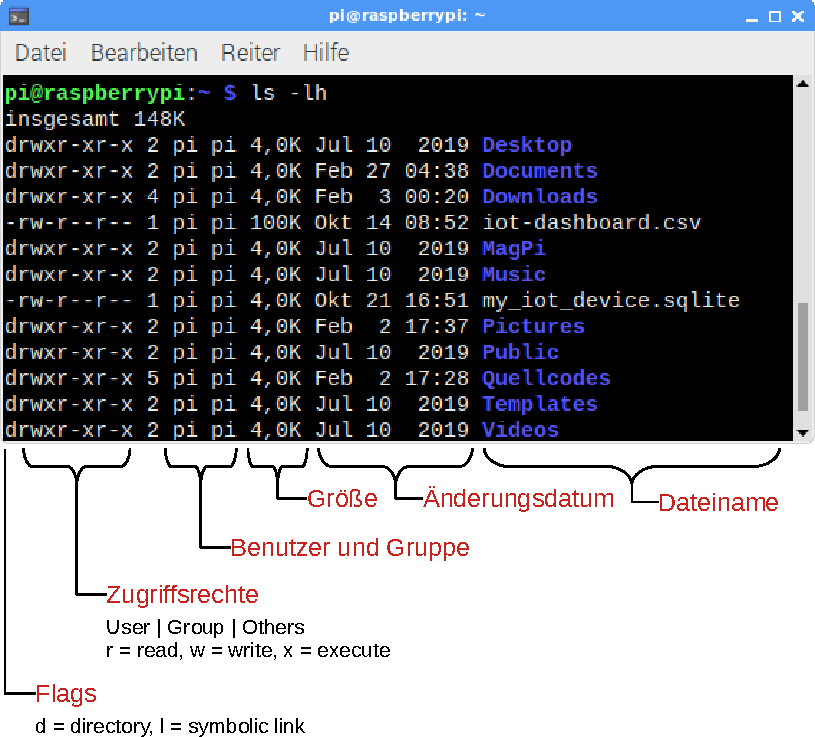
\includegraphics[width=\textwidth]{img/rechte-dateizugriff}

        \column{.4\textwidth}
        \Justified{
            Alle Einträge im Dateisystem sind immer genau einem Benutzerkonto
            und einer Benutzergruppe zugeordnet. Zusätzlich besitzen sie ein
            Bit-Feld mit Zugriffsrechten für

            \begin{itemize}
                \item den Benutzer,
                \item die Benutzergruppe,
                \item den Rest der Welt.
            \end{itemize}

            Über dieses Feld wird gesteuert, ob \mbox{Lese-,} Schreib- oder ausführende
            Zugriffe erlaubt sind.

            \medskip

            \glqq{}Ausführen\grqq{} bedeutet bei einer Datei, diese als Programm
            zu starten. Bei einem Verzeichnis bedeutet es, die Inhalte des
            Verzeichnisses zu sehen.

            \medskip

            Die Berechtigungsprüfung wird immer mit dem Benutzerkonto durchgeführt,
            unter dessen Namen ein zugreifendes Programm läuft.
        }
    \end{columns}

    \bigskip
    \textbf{Wichtige Befehle}
    \medskip

    \begin{columns}[onlytextwidth]
        \column{.3\textwidth}
        \texttt{chown} \\ Benutzer/Gruppe ändern

        \column{.3\textwidth}
        \texttt{chmod} \\ Zugriffsrechte ändern

        \column{.4\textwidth}
        \texttt{sudo} \\ Programm mit anderem Benutzer starten
    \end{columns}
\end{frame}
}

%%% Folie
{
\scriptsize

\begin{frame}{Fallbeispiel: Automatischer Start eines Pythonprogramms}
    \begin{columns}[onlytextwidth]
        \column{.58\textwidth}
        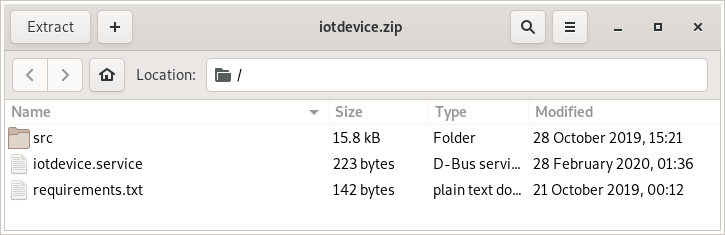
\includegraphics[width=\textwidth]{img/systemd-beispiel-zipfile}

        \column{.4\textwidth}
        \Justified{
            Eine Python-Anwendung soll im Rasbperry Pi OS systemweit installiert
            und beim Hochfahren automatisch gestartet werden. Die Desktop-Umgebung
            (sofern installiert) soll aus Performancegründen deaktiviert werden.
        }
    \end{columns}

    \bigskip
    \textbf{Inhalt der Datei \texttt{iotdevice.service}}
    \lstinputlisting[language=Config]{code/iotdevice.service}

    \medskip
    \textbf{Auszuführende Befehle}
    \vskip -.5em
    \begin{columns}[onlytextwidth]
        \column{.5\textwidth}
        \lstinputlisting[language=Config, linerange={1-8}]{code/iotdevice.install.sh}

        \column{.5\textwidth}
        \lstinputlisting[language=Config, linerange={9-16}, firstnumber=9]{code/iotdevice.install.sh}
    \end{columns}
\end{frame}
}

%-------------------------------------------------------------------------------
\section{Remote-Entwicklung mit VS Code}
%-------------------------------------------------------------------------------

%%% Folien
{
\scriptsize
\setlength{\fboxsep}{0pt}

\begin{frame}[allowframebreaks]{Testen der SSH-Verbindung}
    \begin{center}
        \fbox{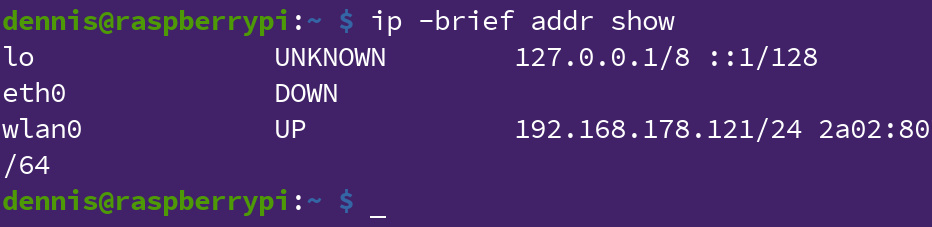
\includegraphics[width=\textwidth]{img/ssh-ip-addr-show}}
    \end{center}

    \Justified{
        Mit dem Befehl \texttt{ip -brief addr show} lassen sich die IP-Adressen des Raspberry Pi anzeigen.
        Diese werden für den Remote-Login mit SSH benötigt, um den Raspberry Pi auch ohne Bildschirm,
        Tastatur und Maus programmieren vom Laptop aus programmieren zu können.
    }

    %%%
    \framebreak

    \begin{center}
        \fbox{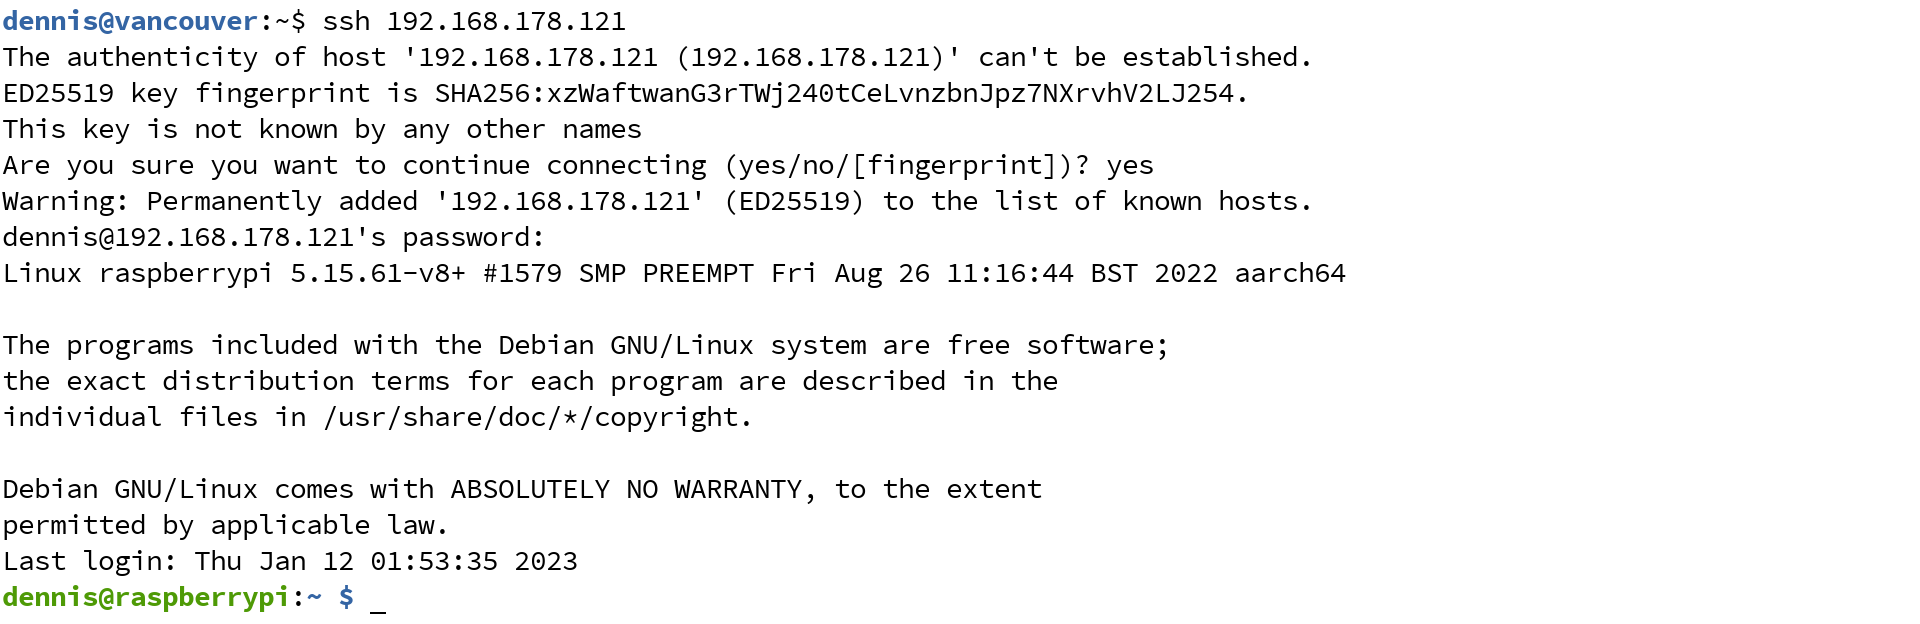
\includegraphics[width=\textwidth]{img/ssh-erstlogon}}
    \end{center}

    \Justified{
        Auf dem eigenen Laptop kann der Logon mit folgendem Befehl getestet werden:
        \smallskip

        \texttt{ssh \textit{benutzername}@\textit{ip-adresse}}
        \smallskip

        Es sollten eine einmalige Sicherheitsabfrage sowie der Login-Prompt des Raspberry Pi
        erscheinen. An diesem sollte man sich mit dem während der Installation angelegten
        Benutzerkonto anmelden können. Mit dem Befehl \texttt{exit} kann die Anmeldung
        danach beendet werden.
        \smallskip

        \textcolor{MidnightBlue}{
            Da sich die IP-Adresse jederzeit ändern kann, werden wir demnächst das Werkzeug
            \textbf{find-my-device} auf dem Raspberry Pi installieren. Damit lässt sich die
            IP-Adresse dann ganz einfach durch Aufrufen einer Webseite ermitteln. Das Werkzeug
            programmiere ich gerade. \smiley{}
            \smallskip
        }

        \textcolor{darkred}{
            Zum Ausschalten führen Sie den Befehl \texttt{sudo poweroff} aus, bevor Sie den
            Strom trennen. EIn hartes Ausschalten ohne diesen Befehl ist nur erlaubt, wenn
            das Dateisystem read-only eingehängt wurde, um Datenverluste zu vermeiden!
        }
    }
\end{frame}
}

%%%%%%%
% TODO: Folien zu "Find my Device"
%%%%%%%

%%% Folien
{
\scriptsize
\setlength{\fboxsep}{0pt}

\begin{frame}[allowframebreaks, fragile]{Remote-Verbindung herstellen}
    \begin{columns}
        \column[c]{.6\textwidth}
        \fbox{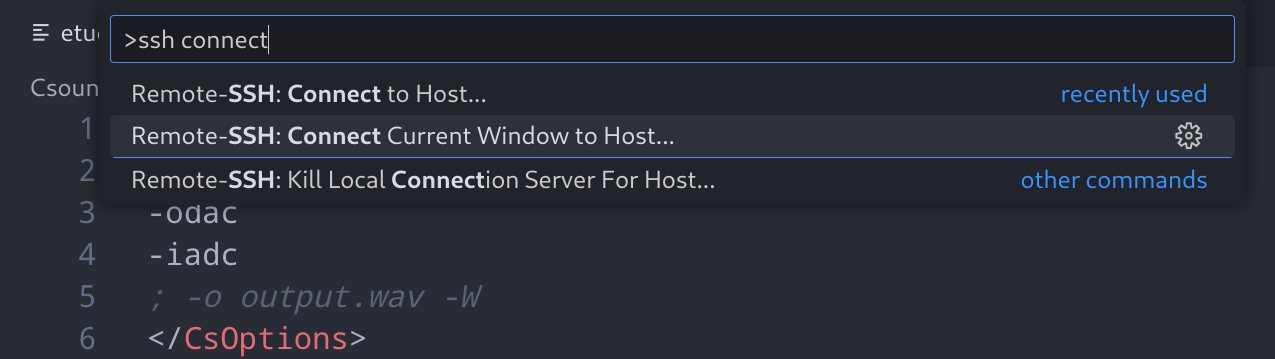
\includegraphics[width=\textwidth]{img/vscode-01}}

        \fbox{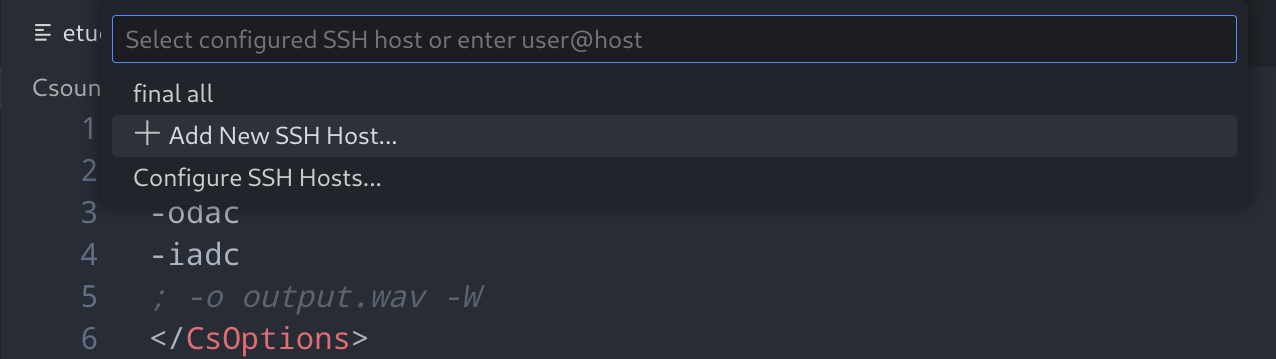
\includegraphics[width=\textwidth]{img/vscode-02}}

        \fbox{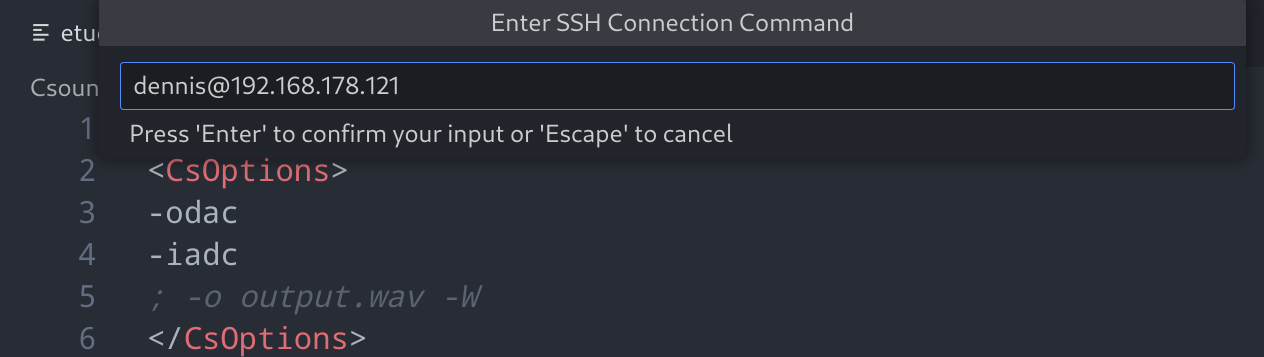
\includegraphics[width=\textwidth]{img/vscode-03}}

        \column[c]{.4\textwidth}
        \Justified{
            Zunächst muss eine neue SSH-Verbindung angelegt werden:
        }

        \begin{enumerate}
            \item Kommandopalette öffnen mit \texttt{Shift+Strg+P}
            \item Nach ,,Remote-SSH'' suchen
            \item Den Eintrag ,,Connect Current Window To Host...'' auswählen
            \item Für die Verbundungsdaten \texttt{\textit{benutzername}@\textit{ip-adresse}} eingeben
        \end{enumerate}
    \end{columns}

    %%%
    \framebreak

    \begin{columns}
        \column[c]{.6\textwidth}
        \fbox{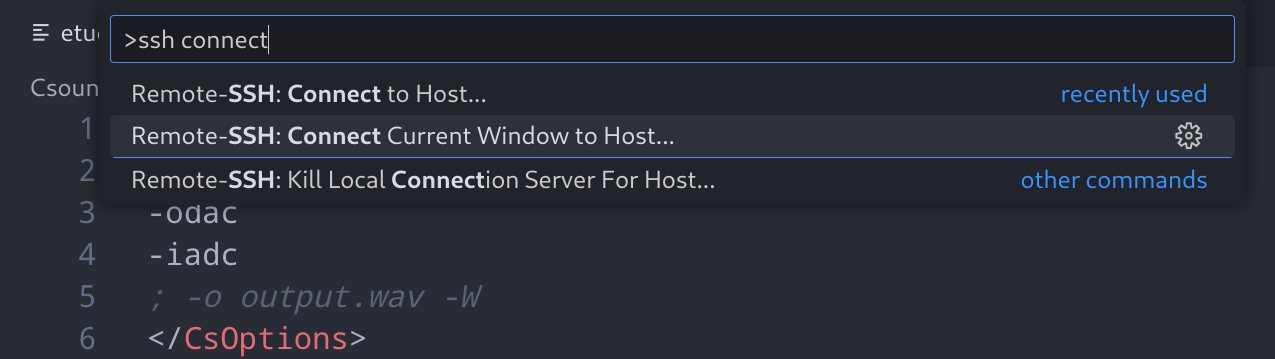
\includegraphics[width=\textwidth]{img/vscode-01}}

        \fbox{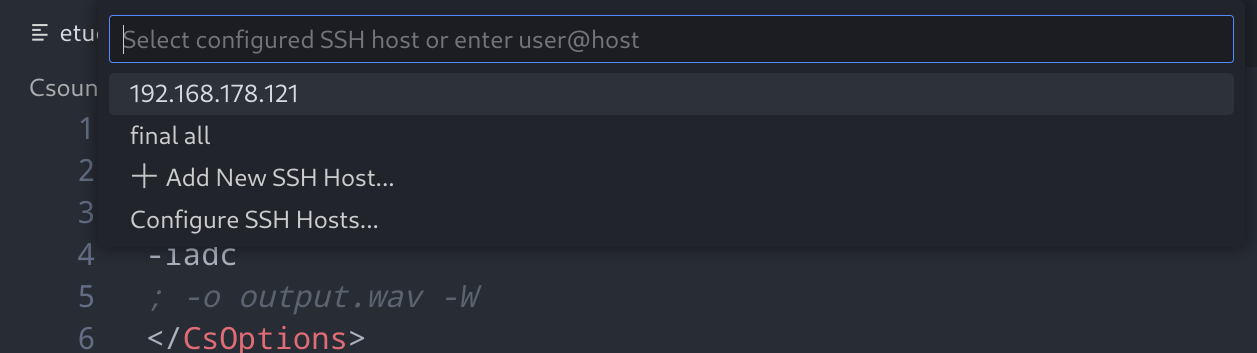
\includegraphics[width=\textwidth]{img/vscode-04}}

        \fbox{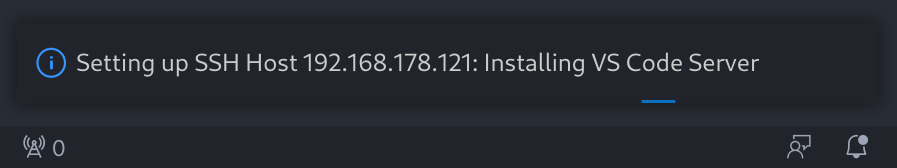
\includegraphics[width=\textwidth]{img/vscode-05}}

        \fbox{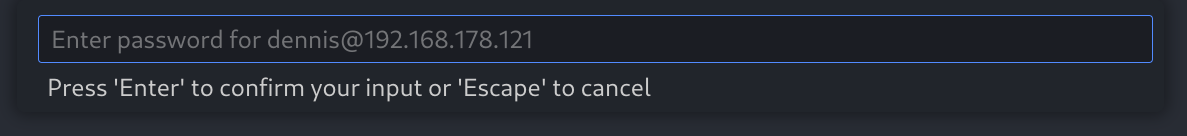
\includegraphics[width=\textwidth]{img/vscode-06}}

        \column[c]{.4\textwidth}
        \Justified{
            Anschließend kann die eben angelegte Verbindung hergestellt werden:
        }

        \begin{enumerate}
            \item Kommandopalette öffnen mit \texttt{Shift+Strg+P}
            \item Erneut nach ,,Remote-SSH'' suchen und ,,Connect Current Window To Host...'' auswählen
            \item Die eben angelegte Verbindung anklicken
            \item Auf Nachfrage das Benutzerpasswort eingeben
            \item Abwarten, bis der Workspace auf dem Raspberry Pi eingerichtet wurde
        \end{enumerate}
    \end{columns}
\end{frame}
}

%%% Folien
{
\scriptsize
\setlength{\fboxsep}{0pt}

\begin{frame}[allowframebreaks, fragile]{Fallbeispiel: Hallo, Raspberry Pi}
    \begin{center}
        \fbox{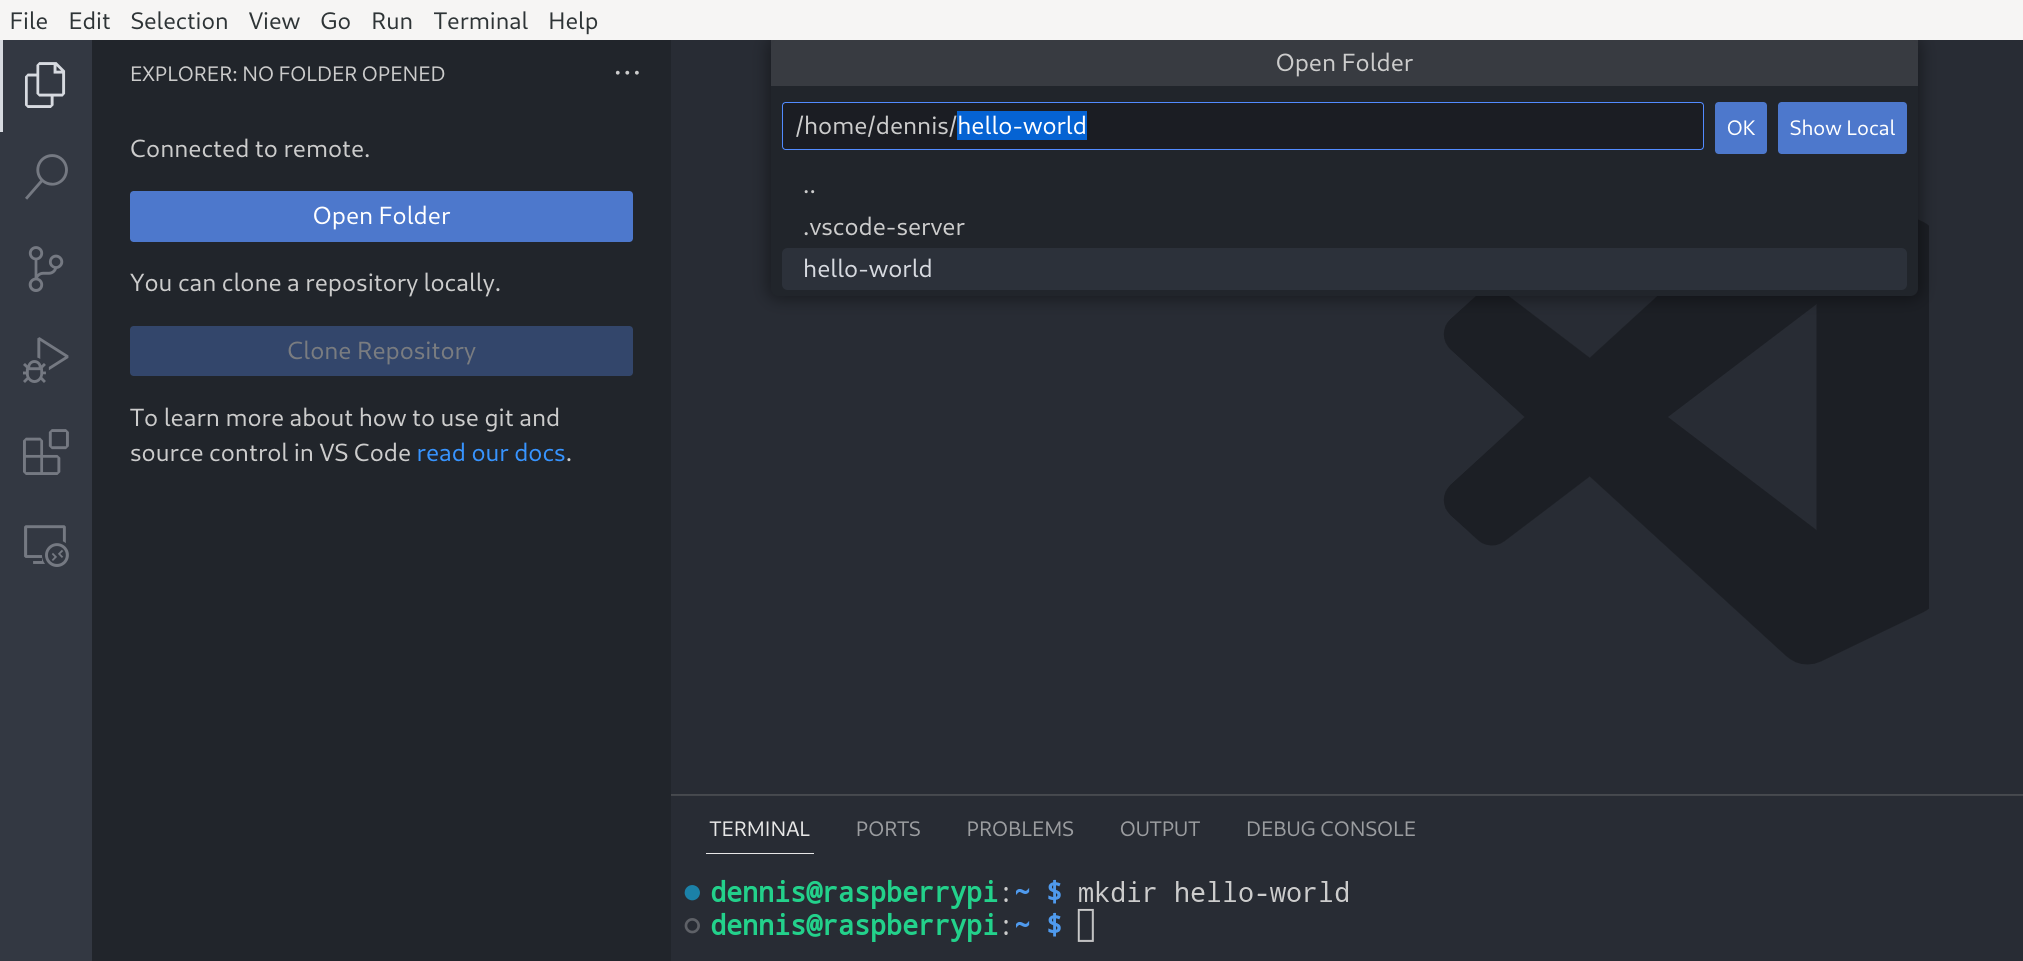
\includegraphics[width=.9\textwidth]{img/vscode-07}}
    \end{center}

    \Justified{
        Mit \texttt{Strg+Ö} (wie englisch ,,Törminal'' \smiley{}) kann eine Konsole geöffnet werden,
        um Befehle auf dem Raspberry Pi auszuführen. Der Befehl \texttt{mkdir \textit{verzeichnis}}
        legt ein neues Quellcodeverzeichnis an, das anschließen über den Button ,,Open Folder''
        im linken Bereich geöffnet werden kann.
    }

    %%%
    \framebreak

    \begin{columns}
        \column[c]{.6\textwidth}
        %~ \fbox{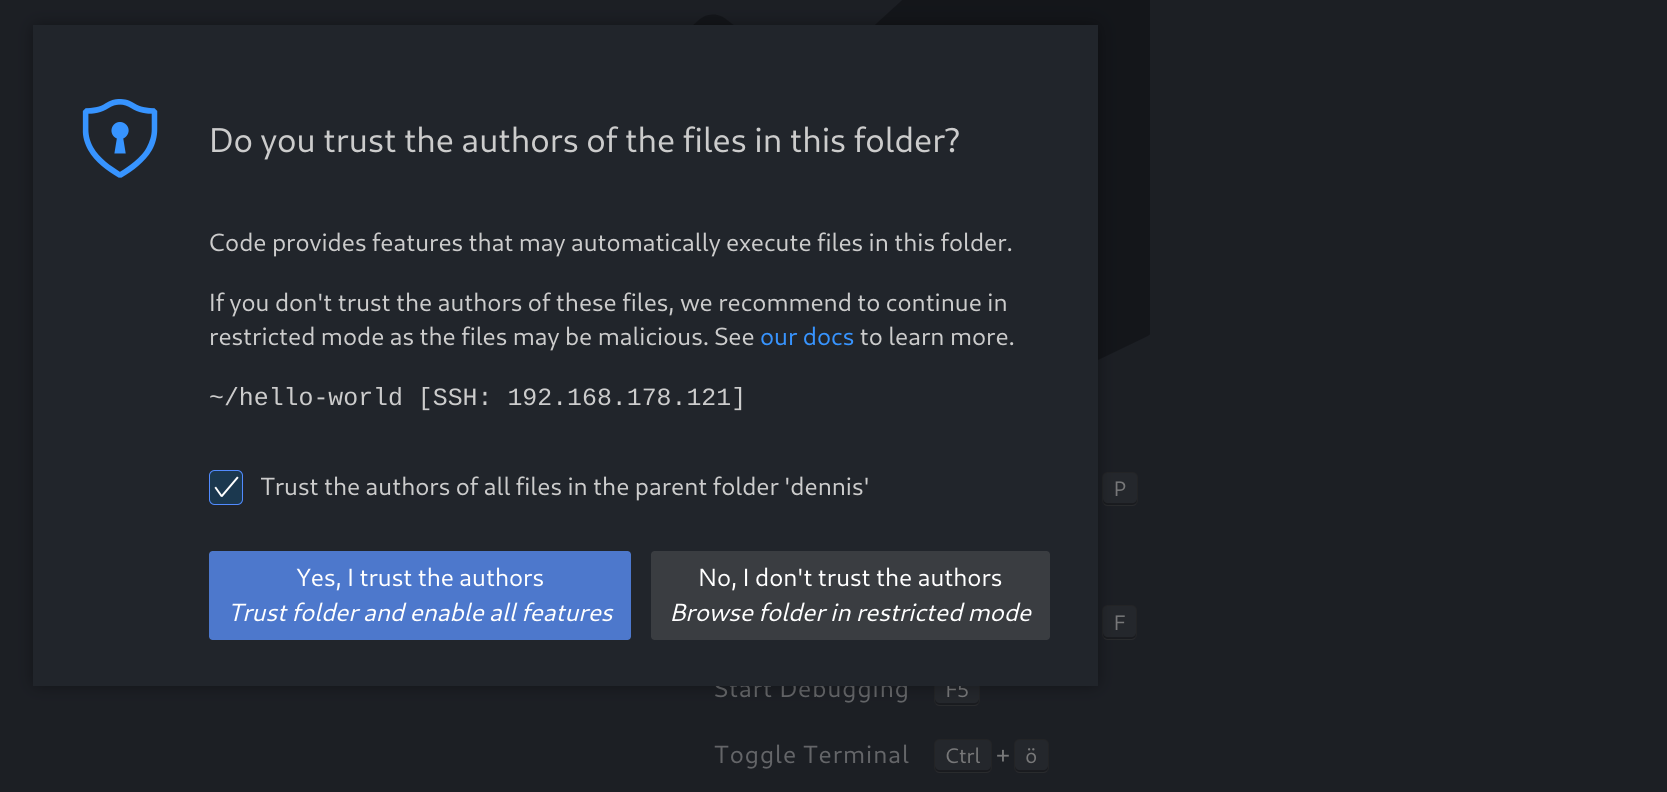
\includegraphics[width=\textwidth]{img/vscode-08}}

        \fbox{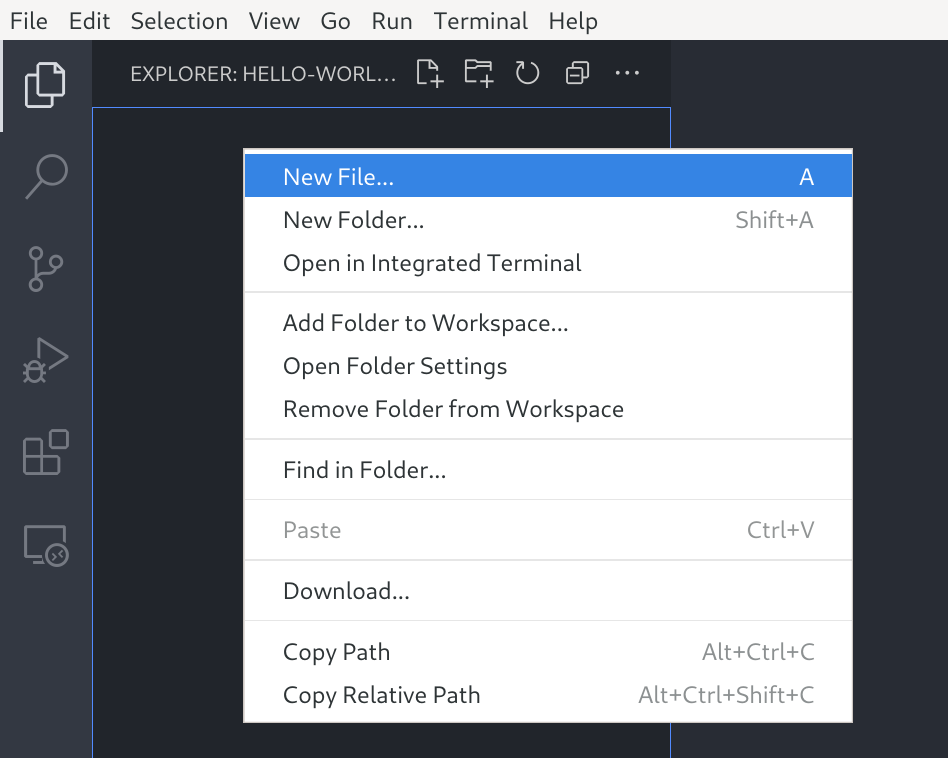
\includegraphics[width=\textwidth]{img/vscode-09}}

        \fbox{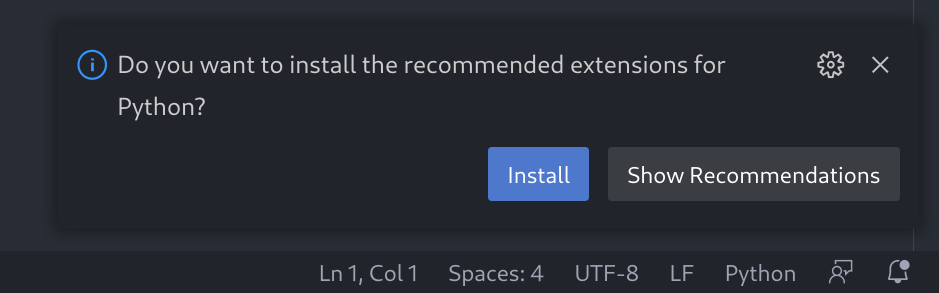
\includegraphics[width=\textwidth]{img/vscode-10}}

        \column[c]{.4\textwidth}
        \Justified{
            Weil das verzeichnis noch leer ist, werden links noch keine Dateien angezeigt.
            Mit Rechtsklick soll daher eine Datei namens \texttt{main.py} angelegt werden.
            \smallskip

            Die Frage, ob die empfohlenen Erweiterungen für die Pythonprogrammierung in
            Visual Studio Code installiert werden sollen, kann mit Klick auf ,,Install''
            bestätigt werden. Die Erweiterungen vereinfachen ein wenig das Programmieren
            durch Codeverschläge und Prüfungen.
        }
    \end{columns}

    %%%
    \framebreak

    \begin{columns}
        \column[c]{.54\textwidth}
        %~ \fbox{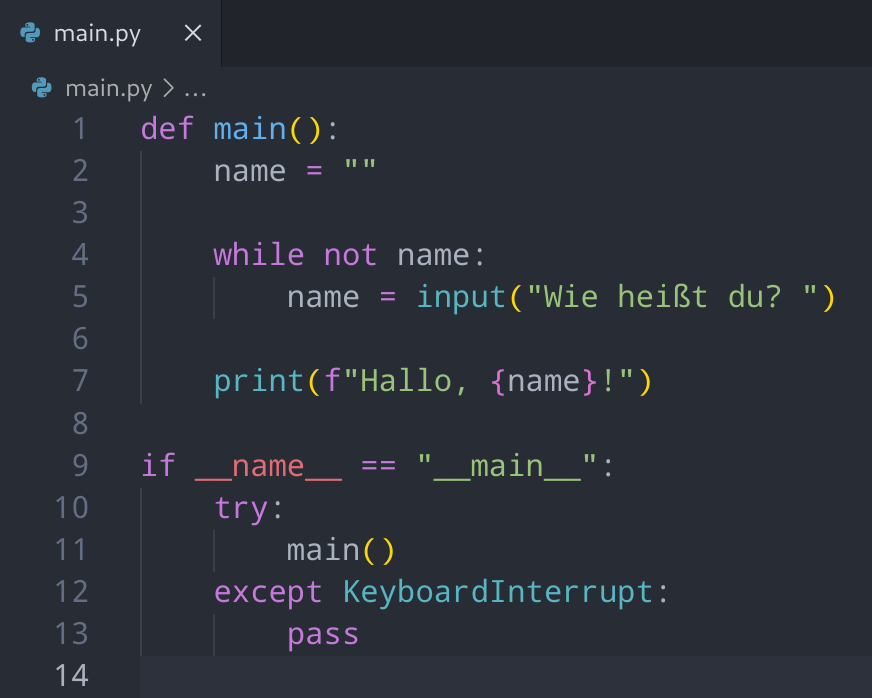
\includegraphics[width=\textwidth]{img/vscode-11}}

        \fbox{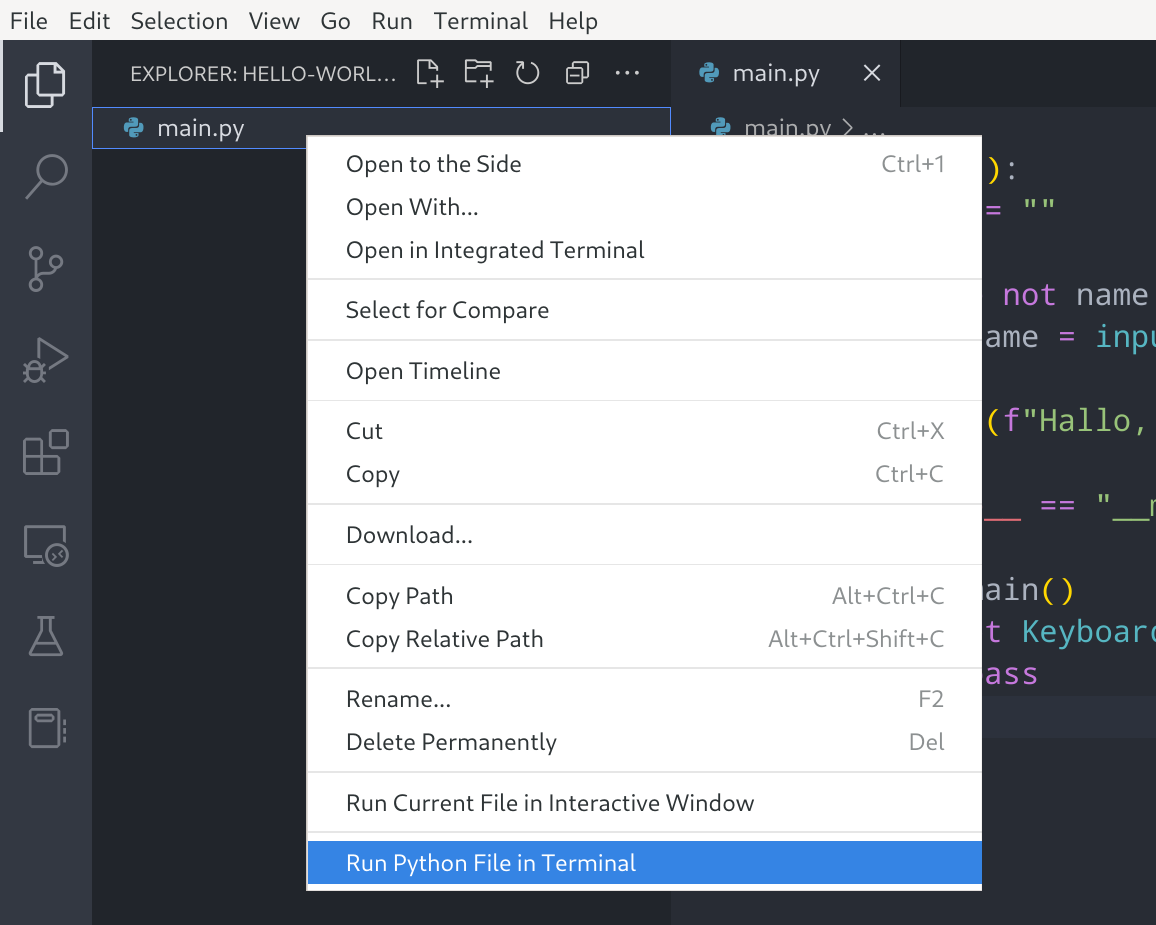
\includegraphics[width=\textwidth]{img/vscode-12}}

        \fbox{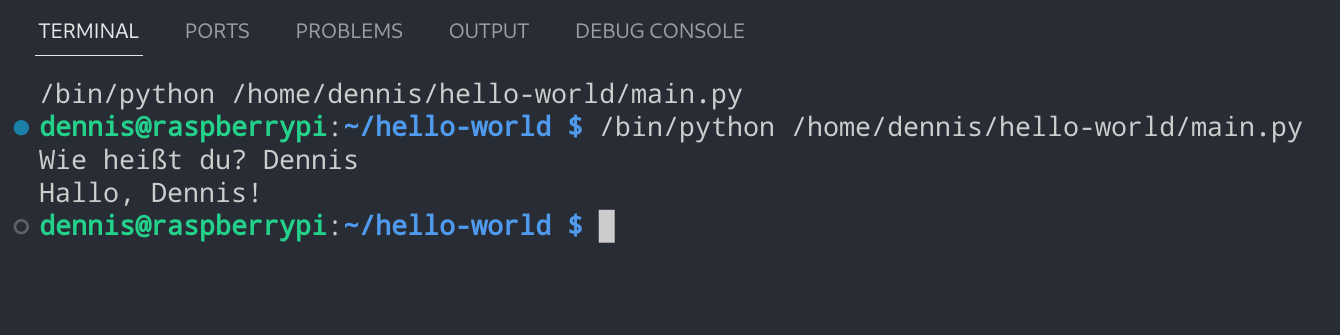
\includegraphics[width=\textwidth]{img/vscode-13}}

        \column[c]{.45\textwidth}
        \Justified{
            Die Datei soll folgenden Inhalt besitzen:
        }

        \begin{lstlisting}[language=Python, gobble=12]
            def main():
                name = ""

                while not name:
                    name = input("Wie heißt du? ")

                print(f"Hallo, {name}!")

            if __name__ == "__main__":
                try:
                    main()
                except KeyboardInterrupt:
                    pass
        \end{lstlisting}

        \bigskip

        \Justified{
            Über den Eintrag ,,Run Python File in Terminal'' im Kontextmenü (Rechtsklick)
            lässt sich das Programm ausführen. Das Ergebnis sollte wie im unteren Screenshot
            aussehen.
        }
    \end{columns}
\end{frame}
}

%-------------------------------------------------------------------------------
\section{Erste Schritte mit Python}
%-------------------------------------------------------------------------------

%%% Folie
\begin{frame}{ChatGPT über Python und Java}
    \begin{center}
        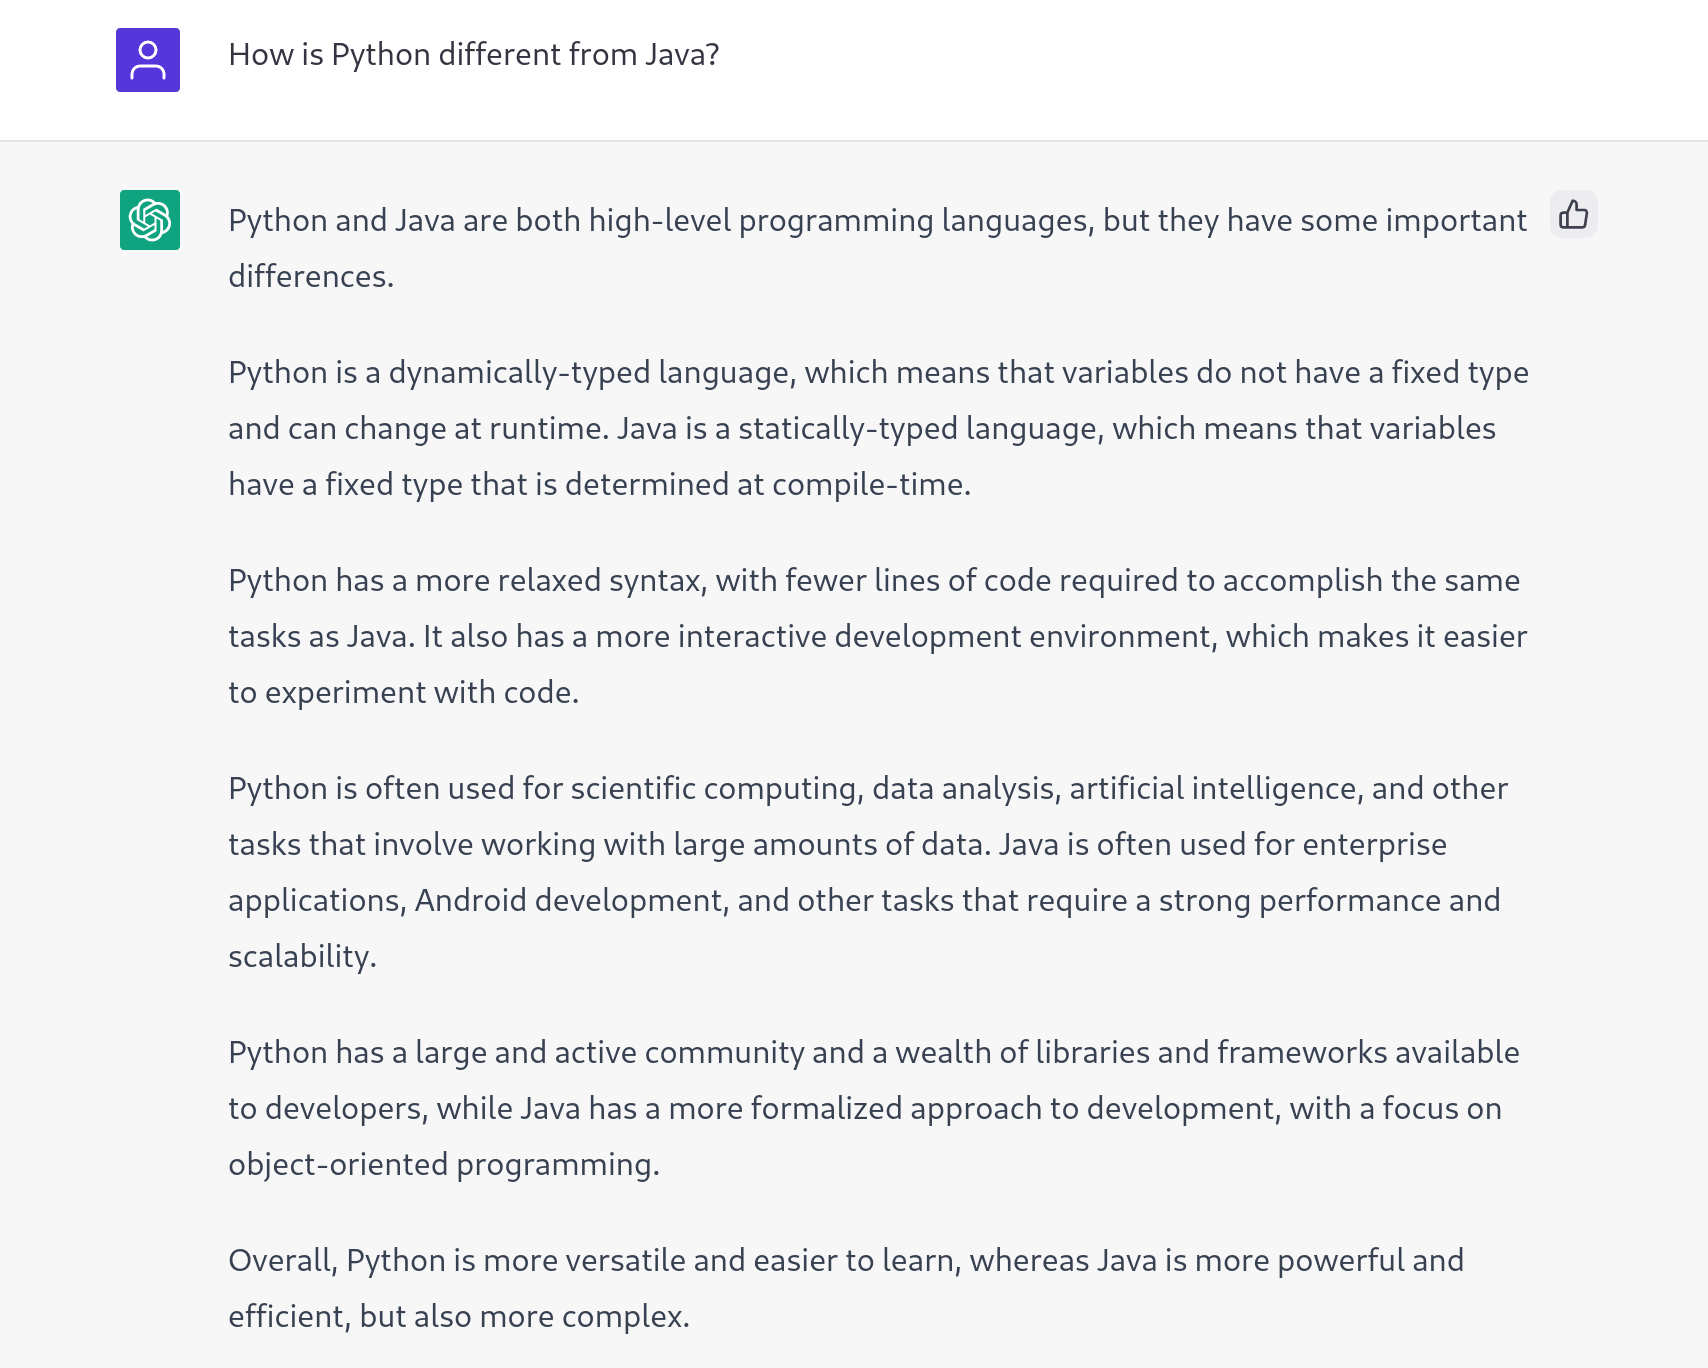
\includegraphics[width=.85\textwidth]{img/chatgpt-python-java}
    \end{center}
\end{frame}

%%% Folie
{
\footnotesize
\setlength{\fboxsep}{0pt}

\begin{frame}{Hilfreiche Webseiten über Python}
    \begin{columns}
        \column[T]{.33\textwidth}
        \fbox{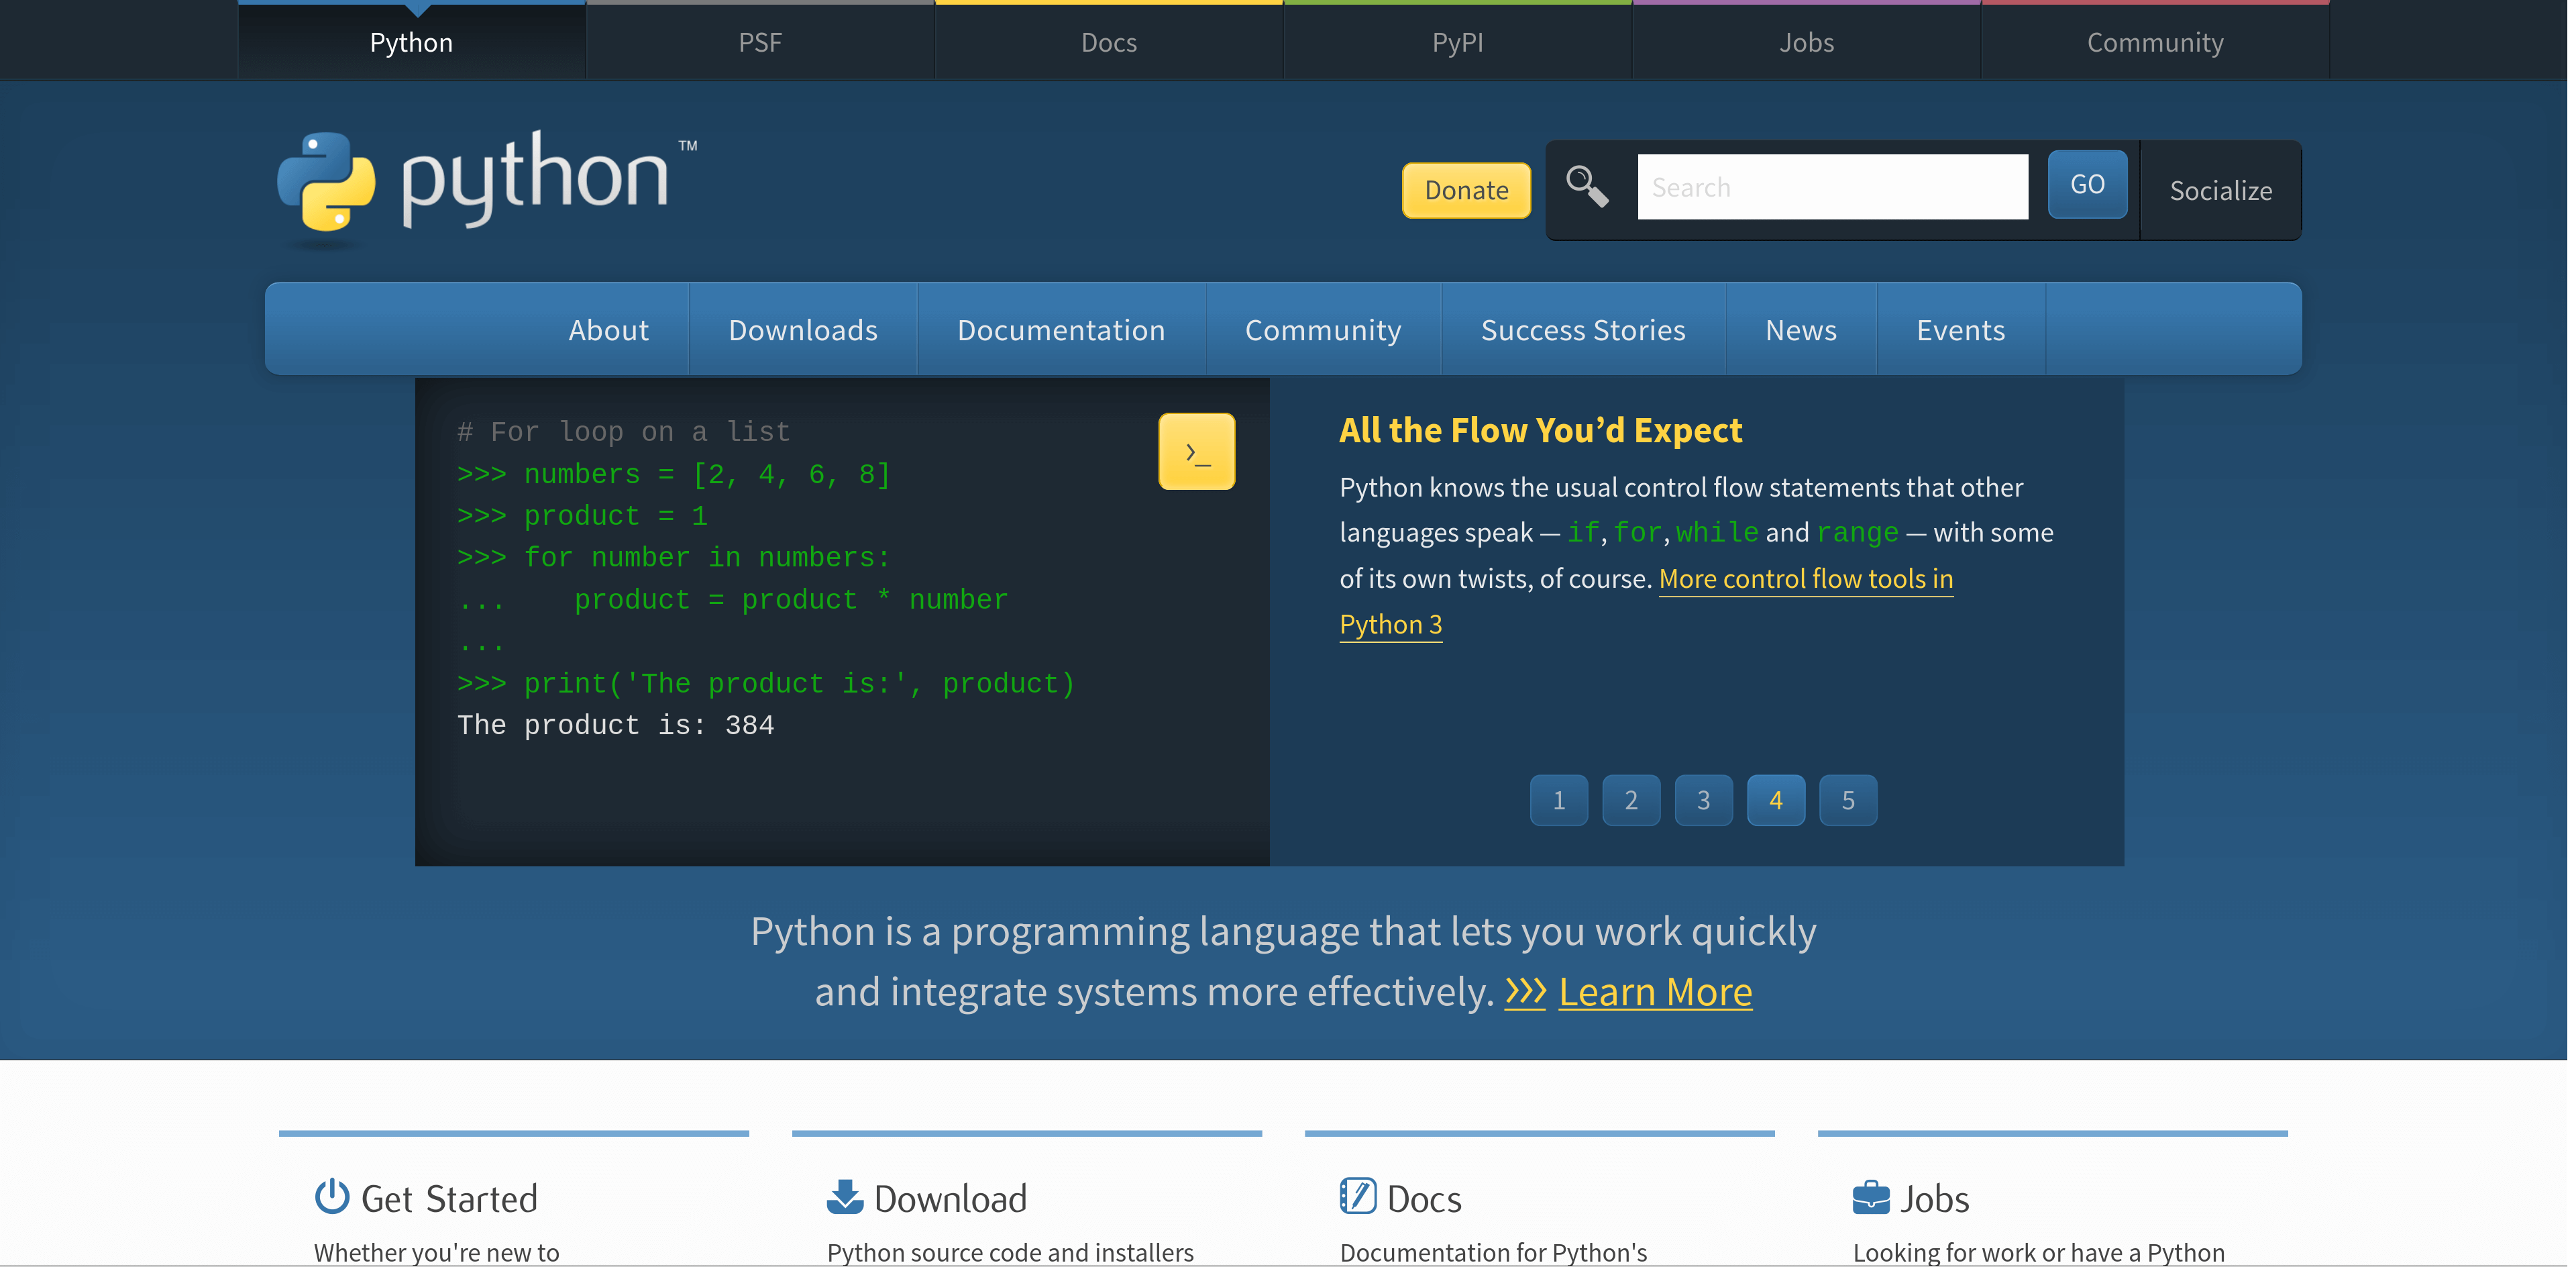
\includegraphics[width=\textwidth]{img/webseite-python}}
        \vskip .5em
        \textbf{Webseite von Python} \\
        \href{https://www.python.org/}{python.org}

        \column[T]{.33\textwidth}
        \fbox{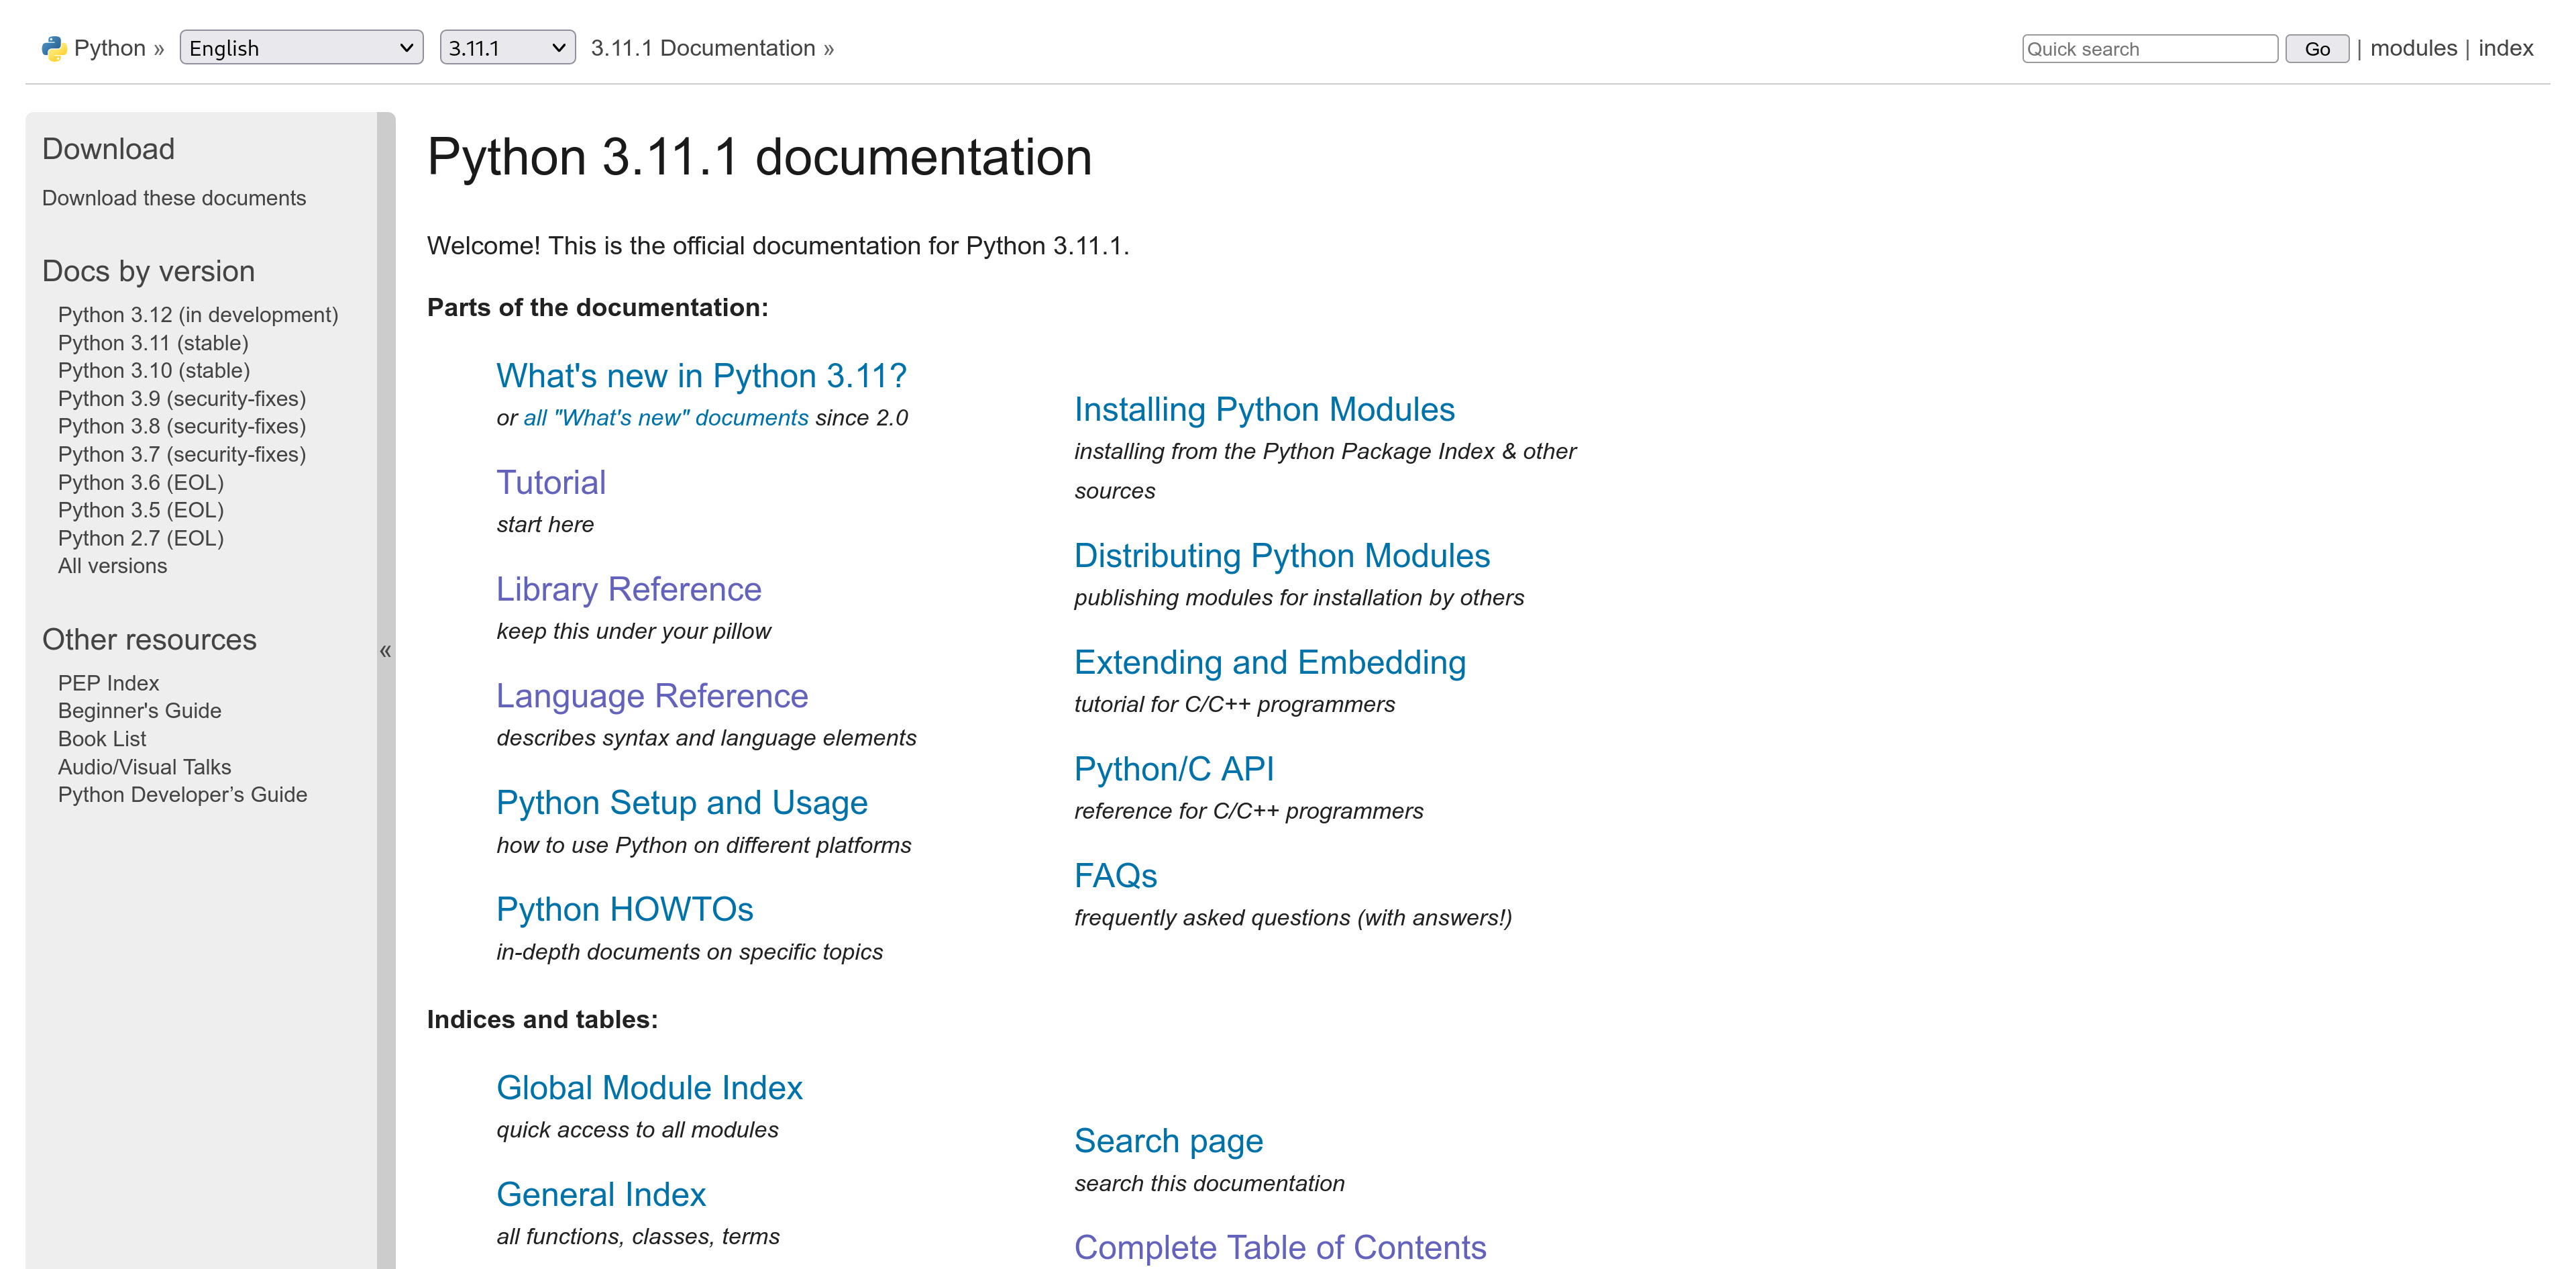
\includegraphics[width=\textwidth]{img/webseite-docs}}
        \vskip .5em
        \textbf{Offizielle Dokumentation} \\
        \href{https://docs.python.org/}{docs.python.org}

        \column[T]{.33\textwidth}
        \fbox{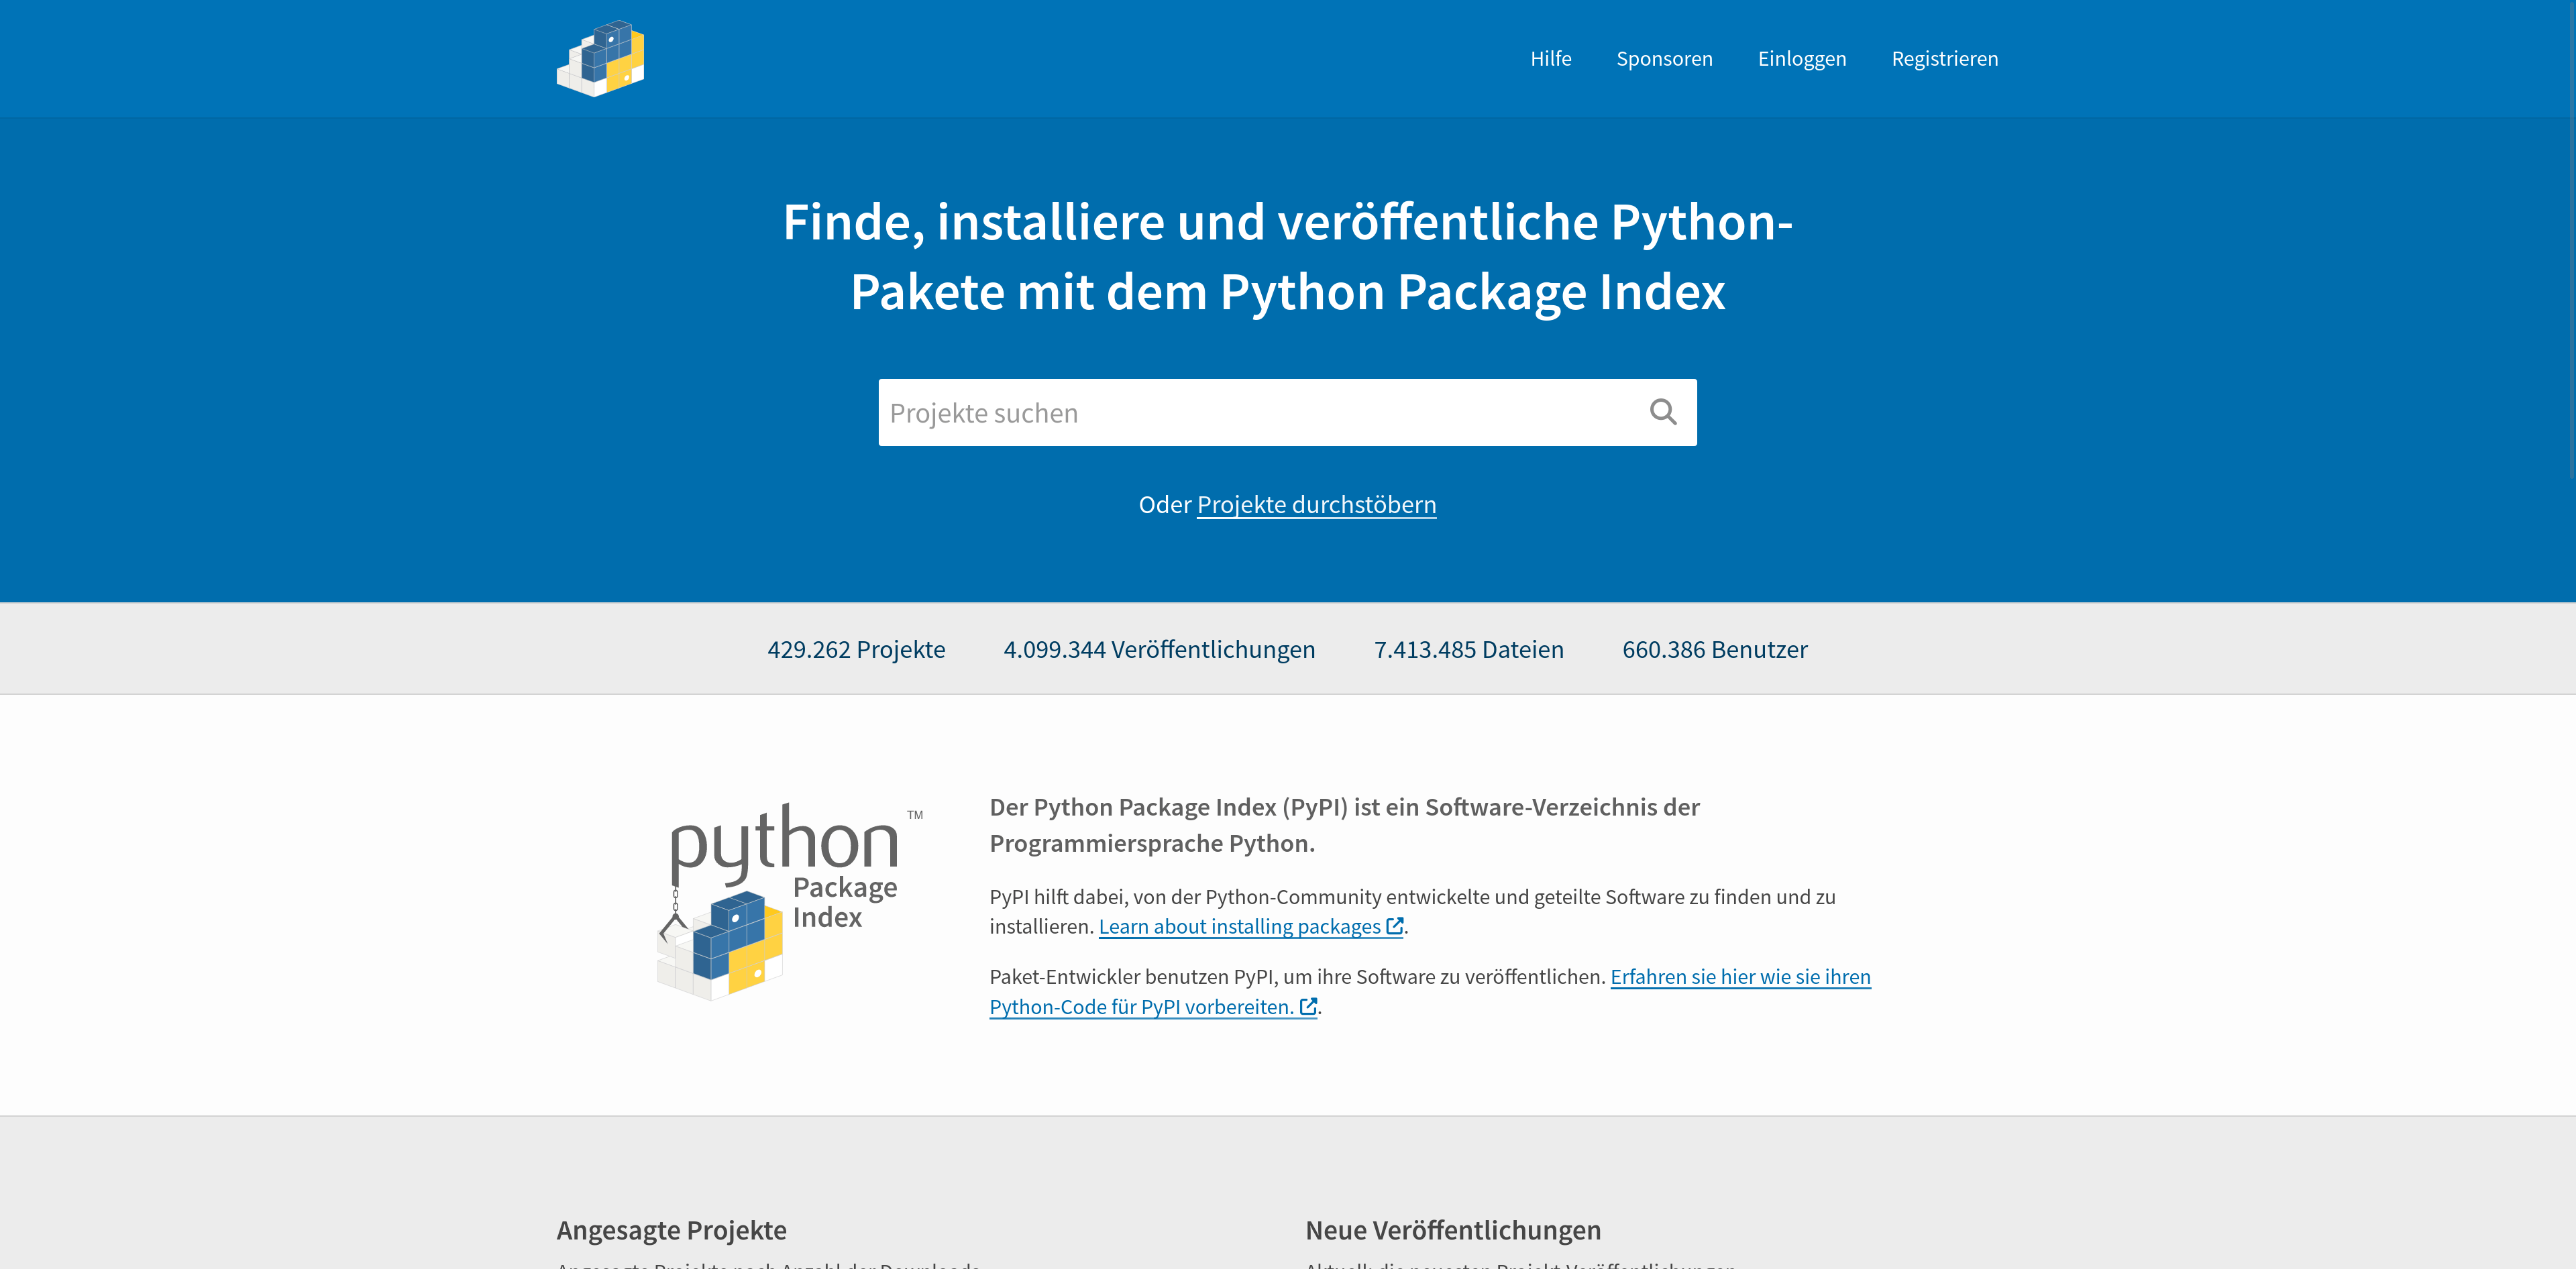
\includegraphics[width=\textwidth]{img/webseite-pypi}}
        \vskip .5em
        \textbf{Python Package Index} \\
        \href{https://pypi.org/}{pypi.org}
    \end{columns}

    \vskip 0.6cm

    \begin{columns}
        \column[T]{.33\textwidth}
        \fbox{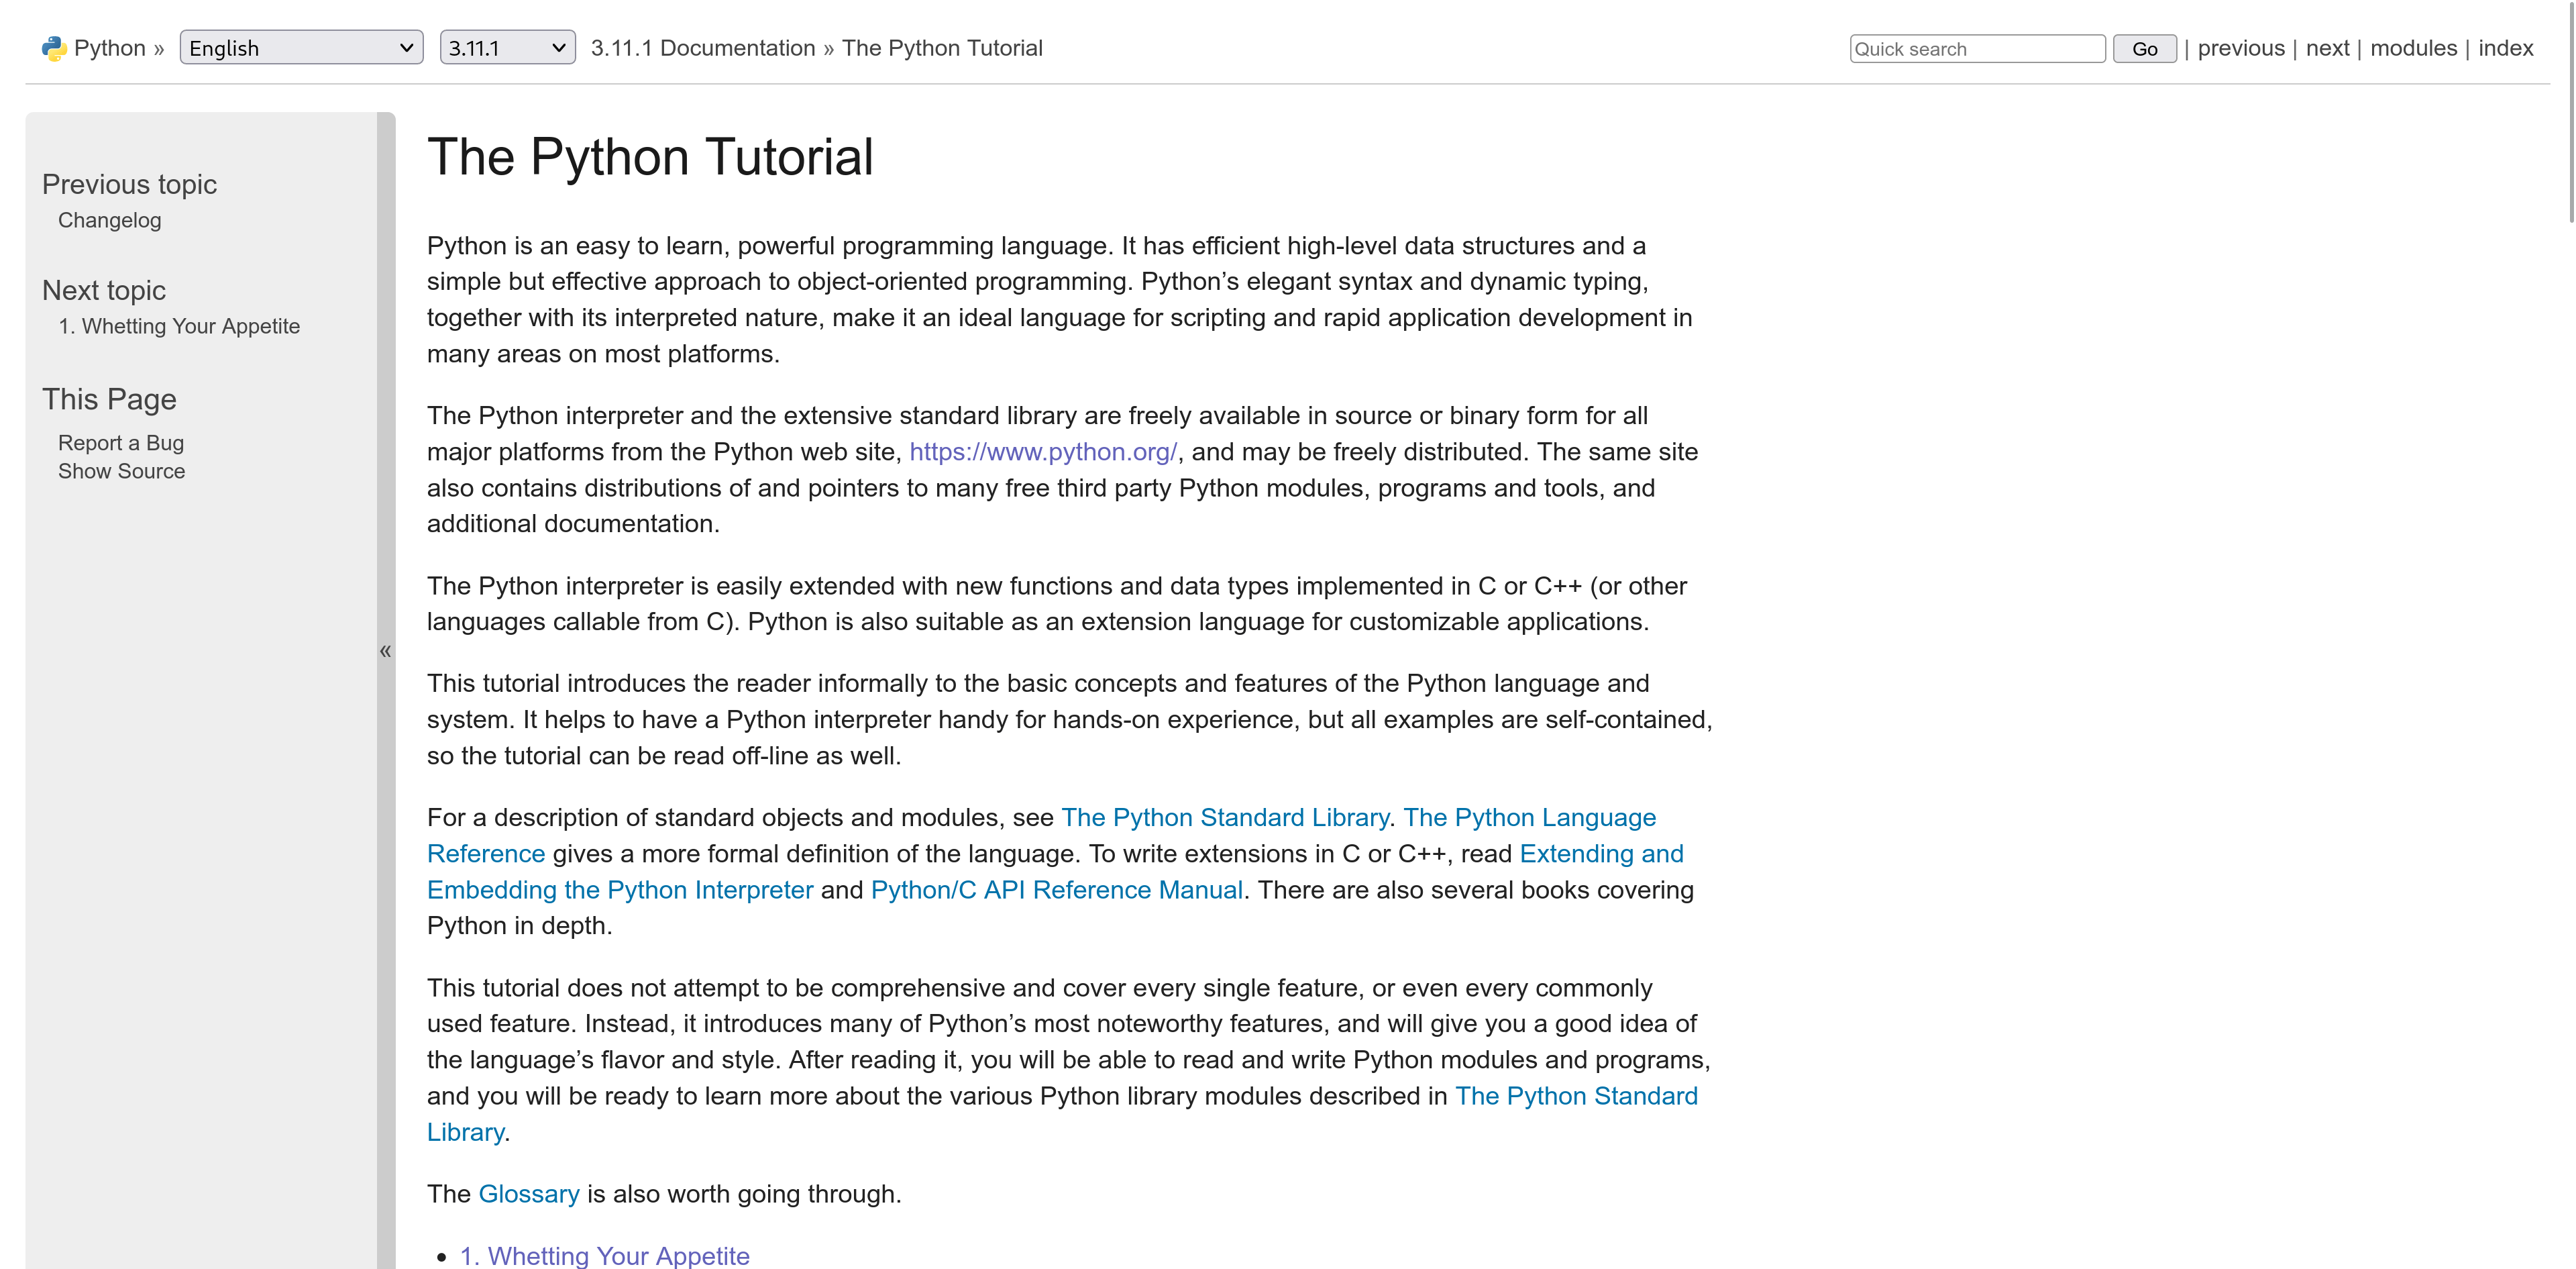
\includegraphics[width=\textwidth]{img/webseite-tuten}}
        \vskip .5em
        \textbf{Englisches Tutorial} \\
        \href{https://docs.python.org/3/tutorial/}{docs.python.org/3/tutorial/}

        \column[T]{.33\textwidth}
        \fbox{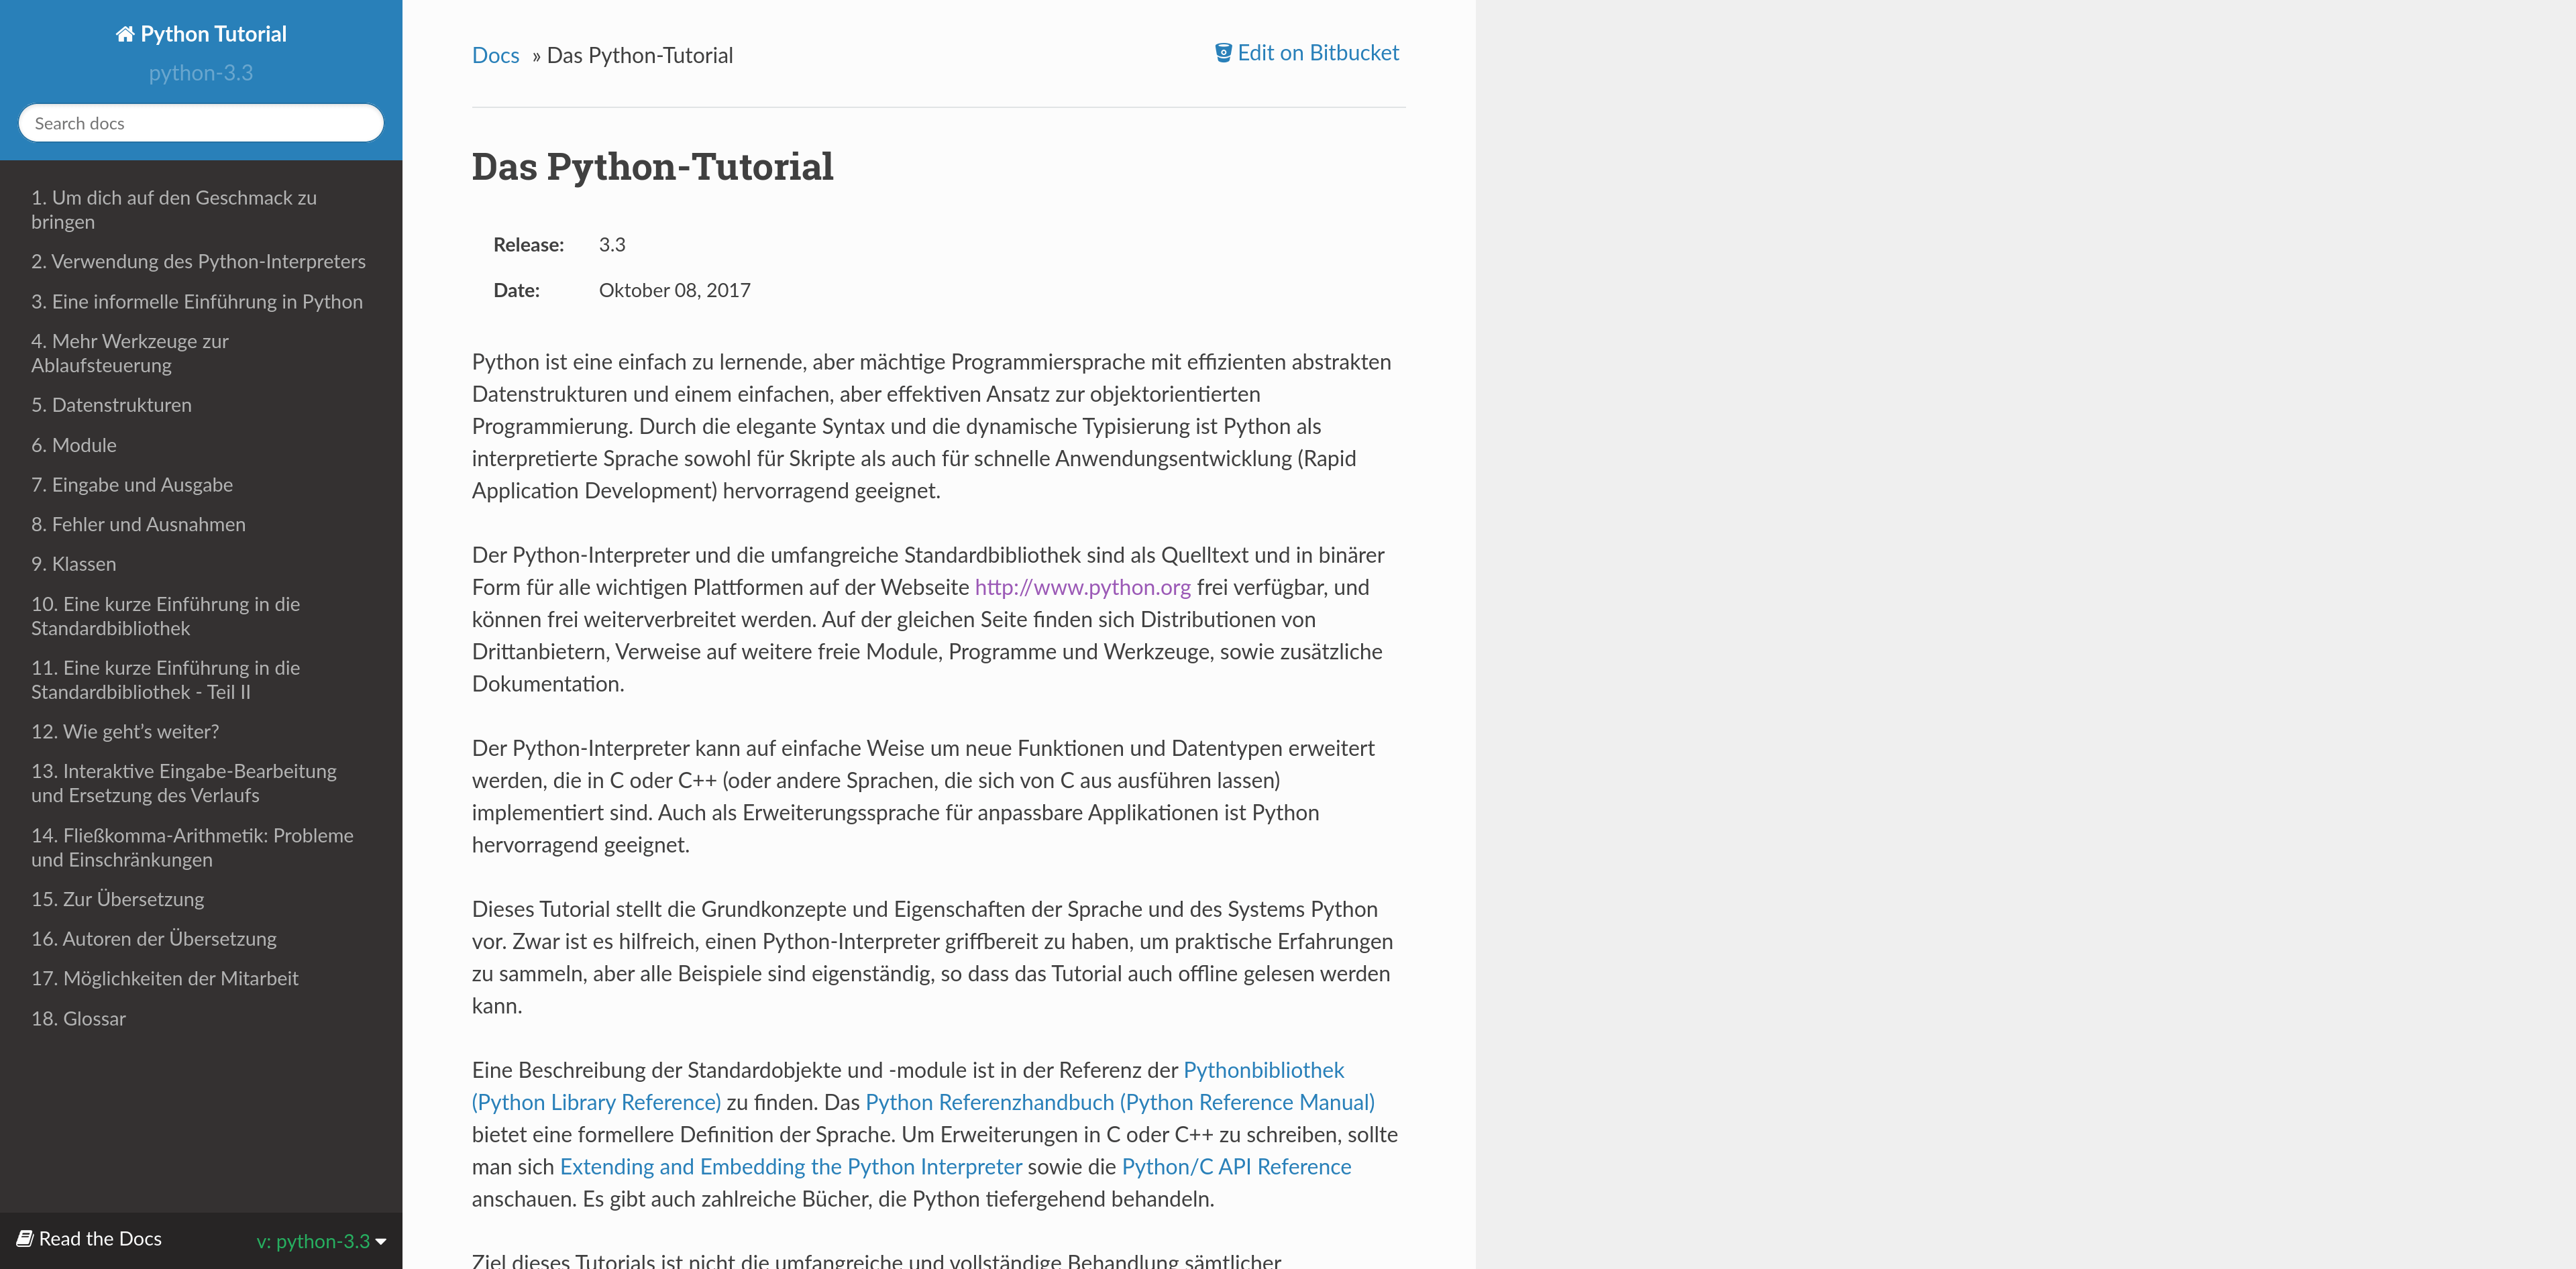
\includegraphics[width=\textwidth]{img/webseite-tutde}}
        \vskip .5em
        \textbf{Deutsches Tutorial} \\
        \href{https://py-tutorial-de.readthedocs.io/}{py-tutorial-de.readthedocs.io}

        \column[T]{.33\textwidth}
        \fbox{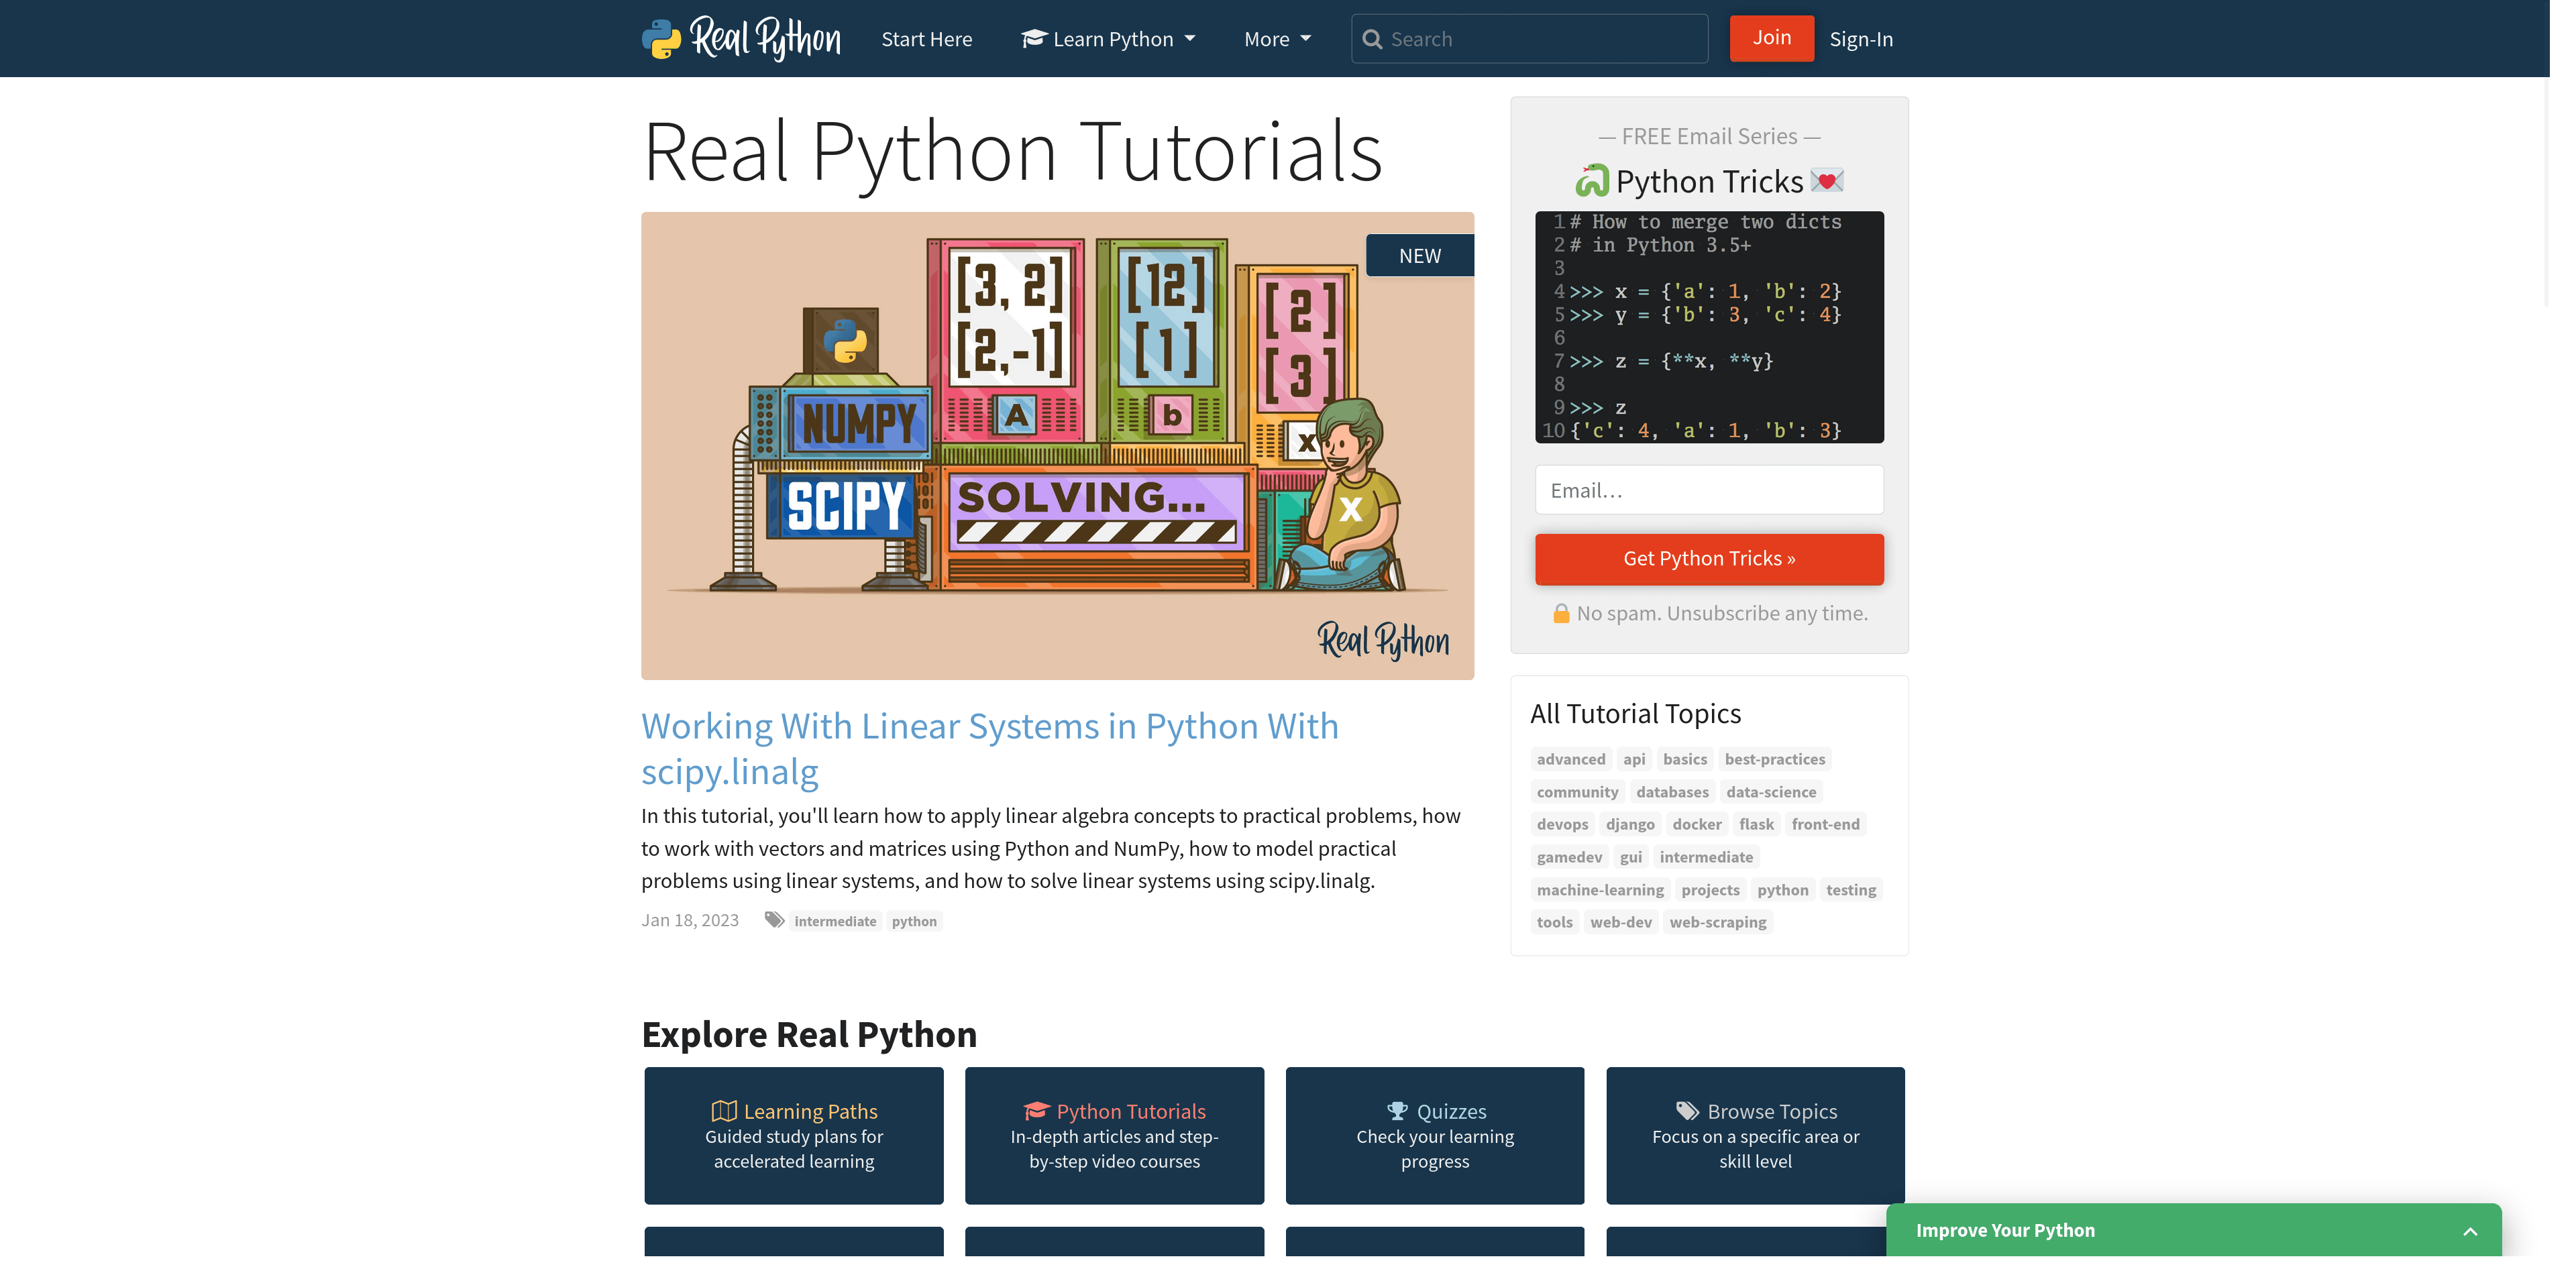
\includegraphics[width=\textwidth]{img/webseite-realpython}}
        \vskip .5em
        \textbf{Real Python} \\
        \href{https://realpython.com/}{realpython.com}
    \end{columns}
\end{frame}
}

%%%%%%%%%%%%%%%%%%%%%%%%%%%%%%%%%
%%%%% TODO: Weitere Folien %%%%%%
%%%%%%%%%%%%%%%%%%%%%%%%%%%%%%%%%

%%% Folie
\begin{frame}[allowframebreaks]{ChatGPT über Duck Typing}
    \begin{center}
        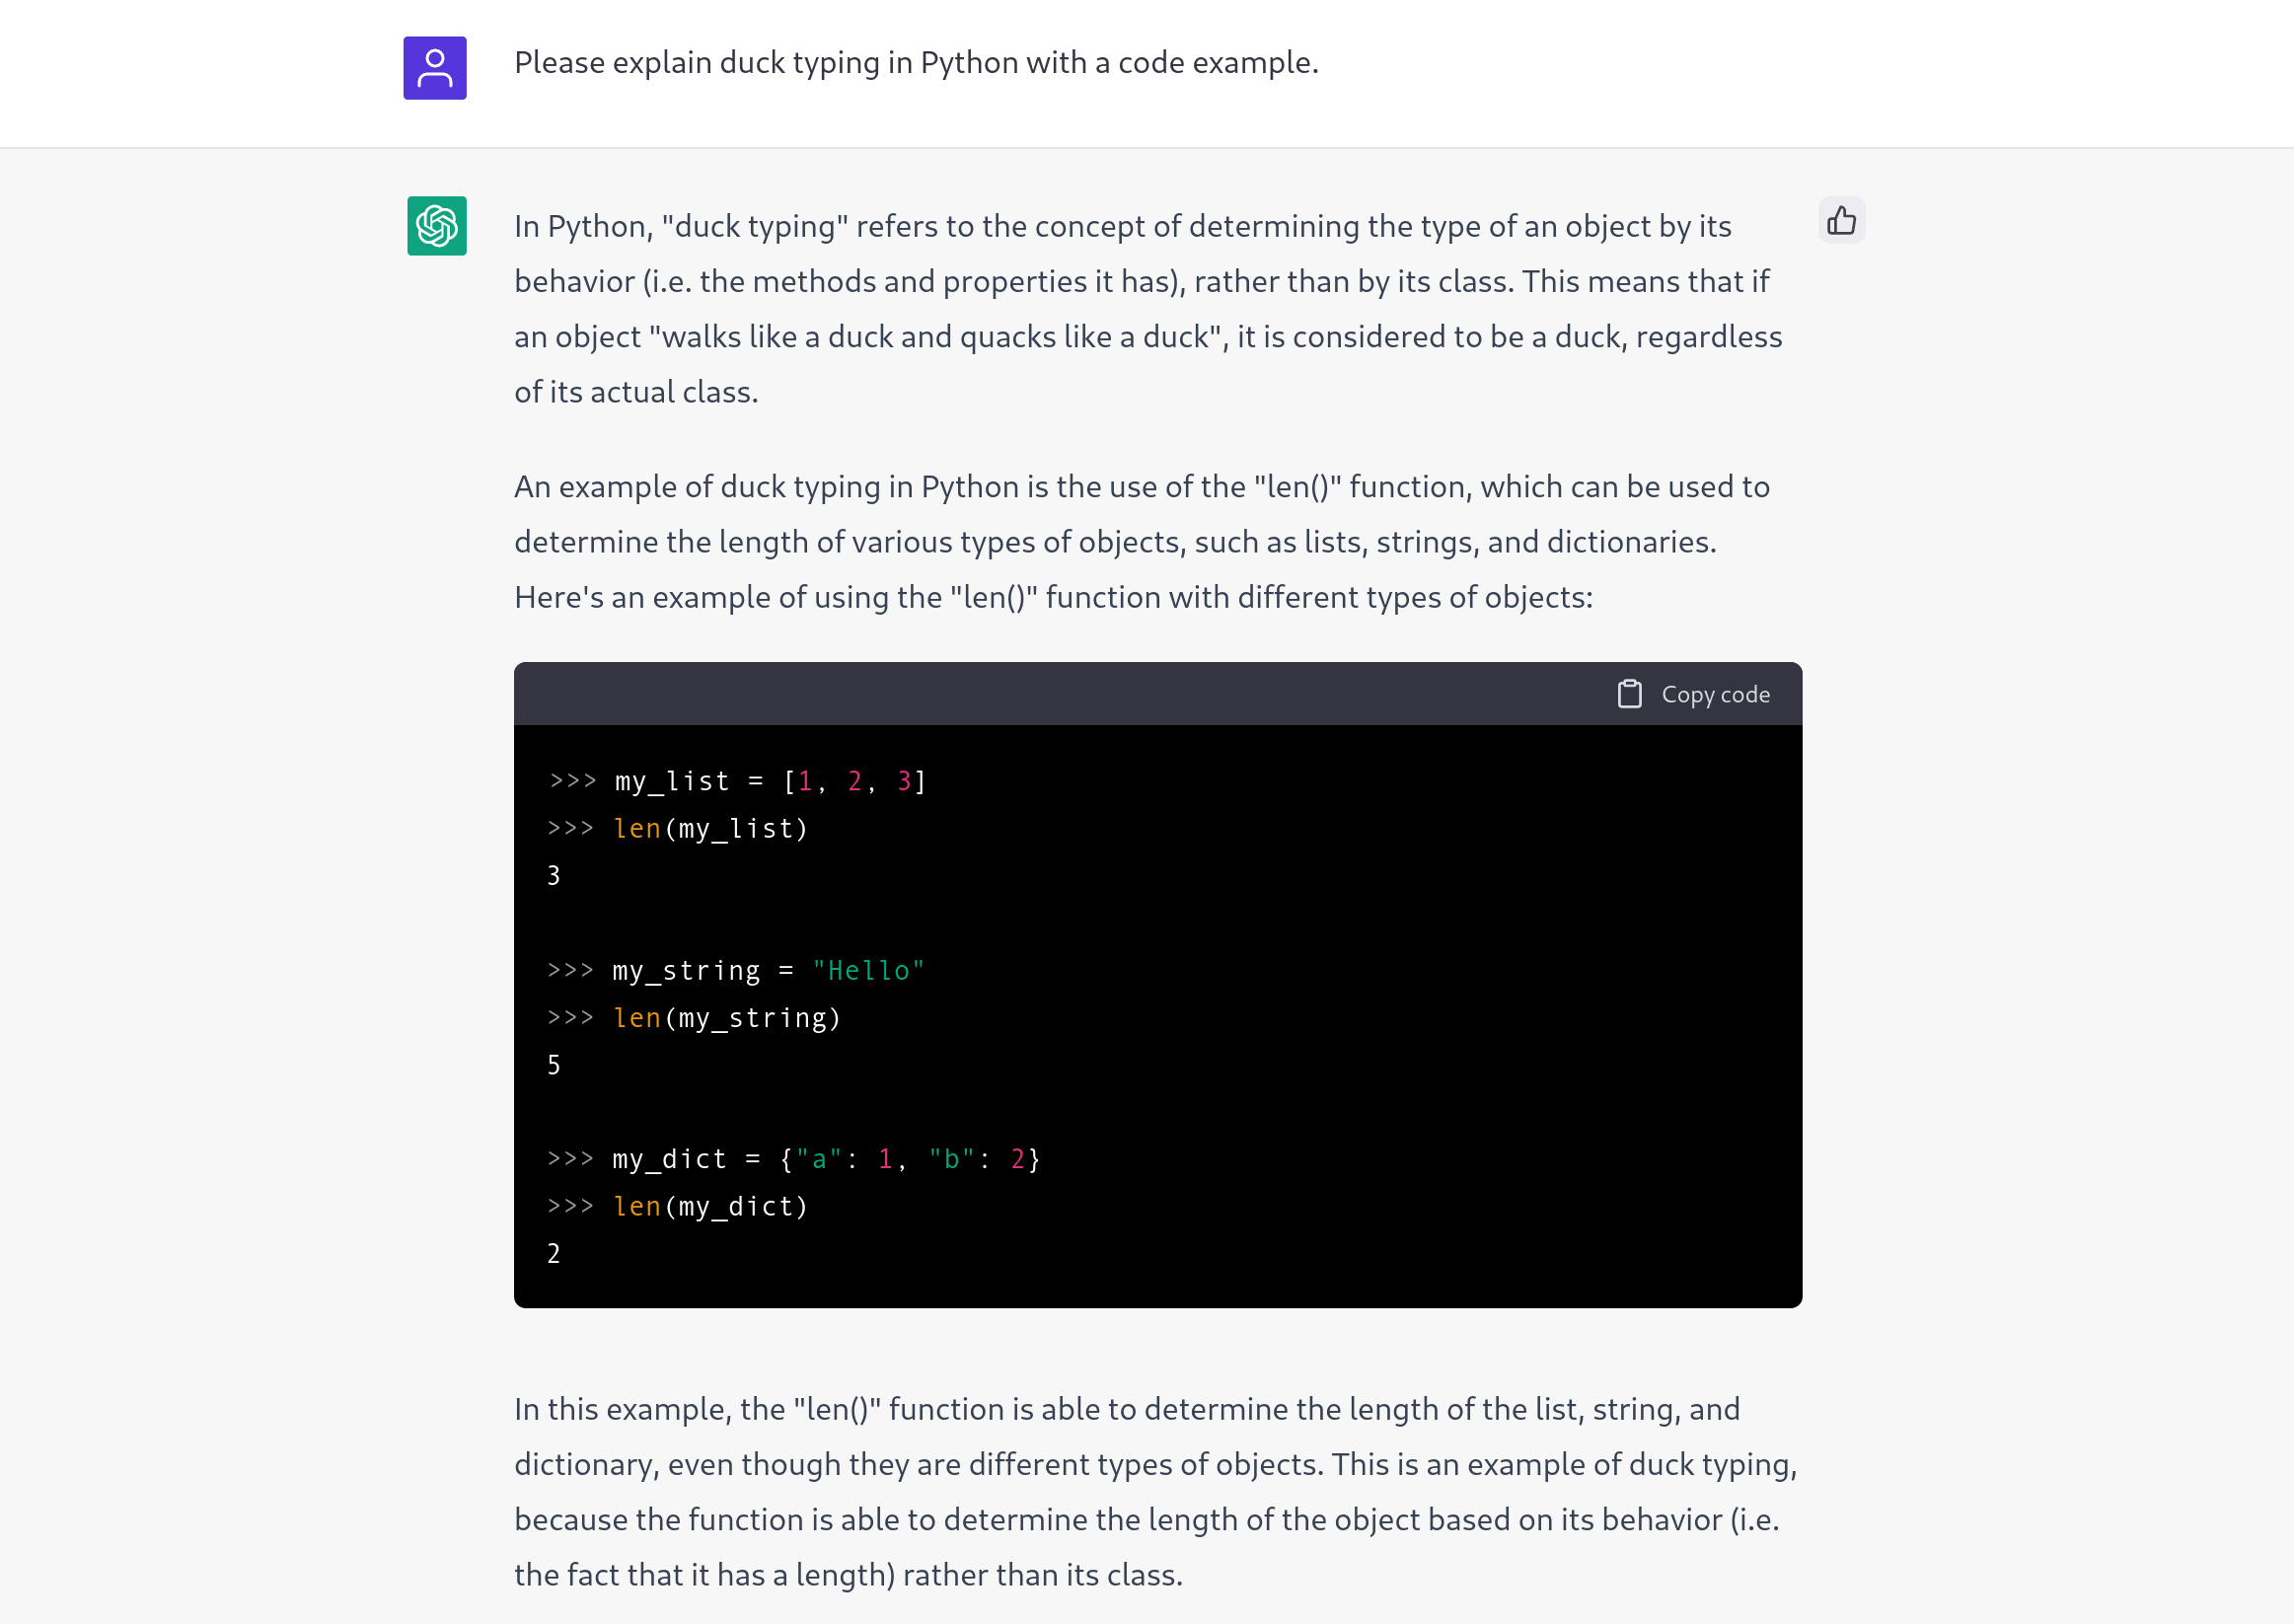
\includegraphics[width=.9\textwidth]{img/chatgpt-ducktyping1}
    \end{center}

    %%%
    \framebreak

    \begin{center}
        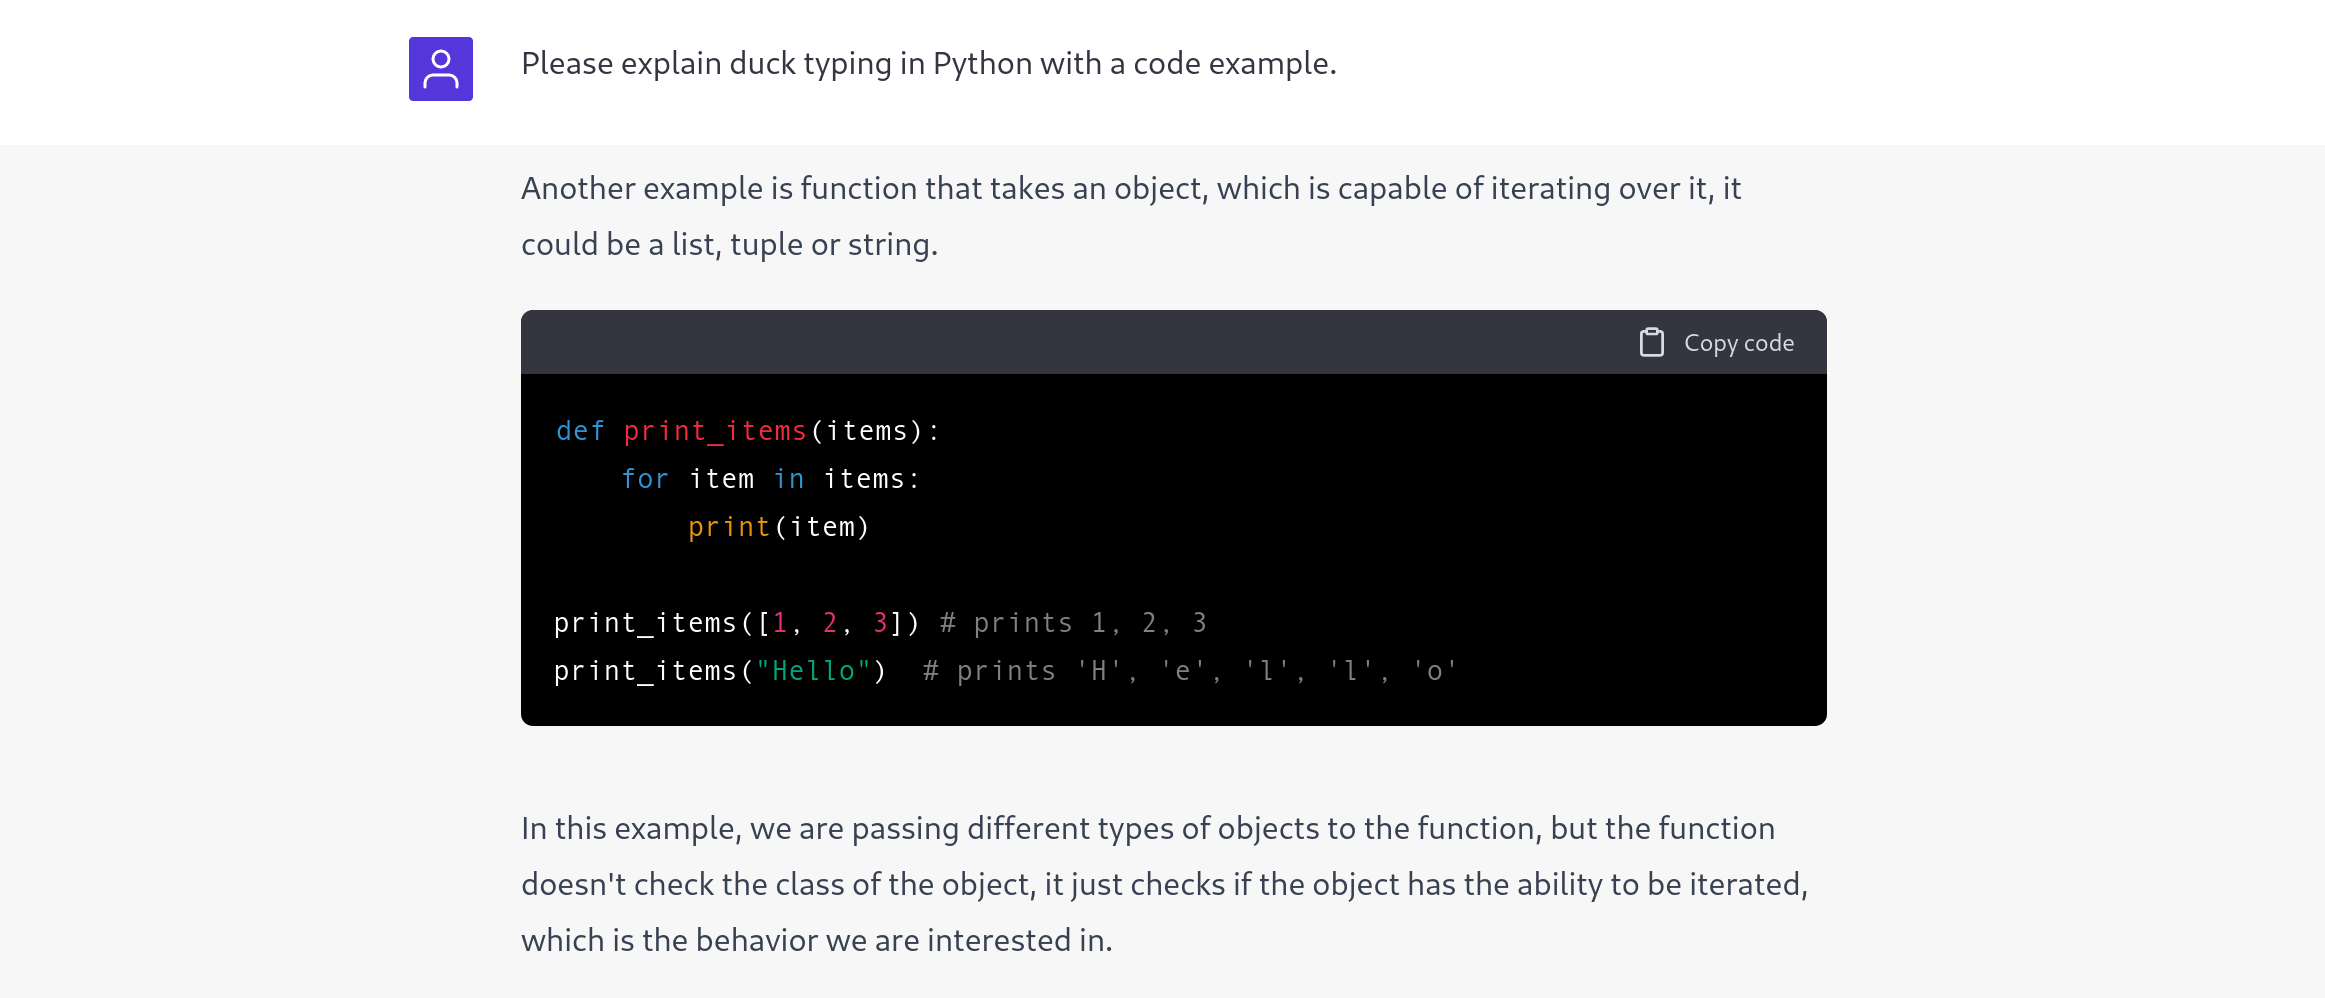
\includegraphics[width=.9\textwidth]{img/chatgpt-ducktyping2}
    \end{center}
\end{frame}

%%%%%%%%%%%%%%%%%%%%%%%%%%%%%%%%%
%%%%% TODO: Weitere Folien %%%%%%
%%%%%%%%%%%%%%%%%%%%%%%%%%%%%%%%%

%%% Folie
\begin{frame}{Ergebnis unseres kleinen Programms}
    \begin{columns}
        \column[T]{.4\textwidth}
        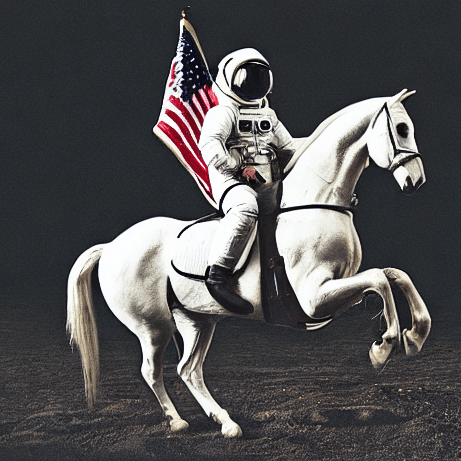
\includegraphics[width=\textwidth]{img/ai-gallery1}

        \column[T]{.4\textwidth}
        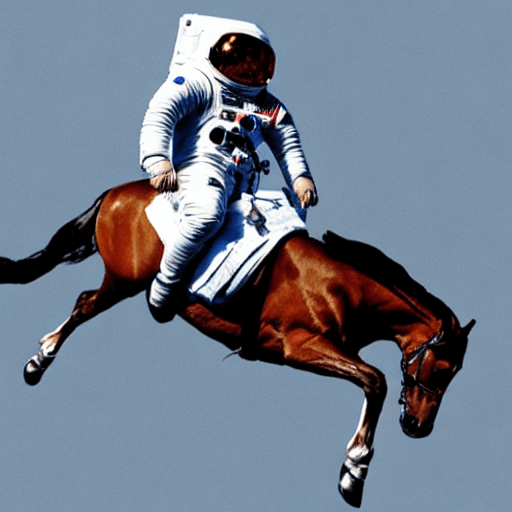
\includegraphics[width=\textwidth]{img/ai-gallery2}
    \end{columns}

    \begin{columns}
        \column[T]{.8\textwidth}
        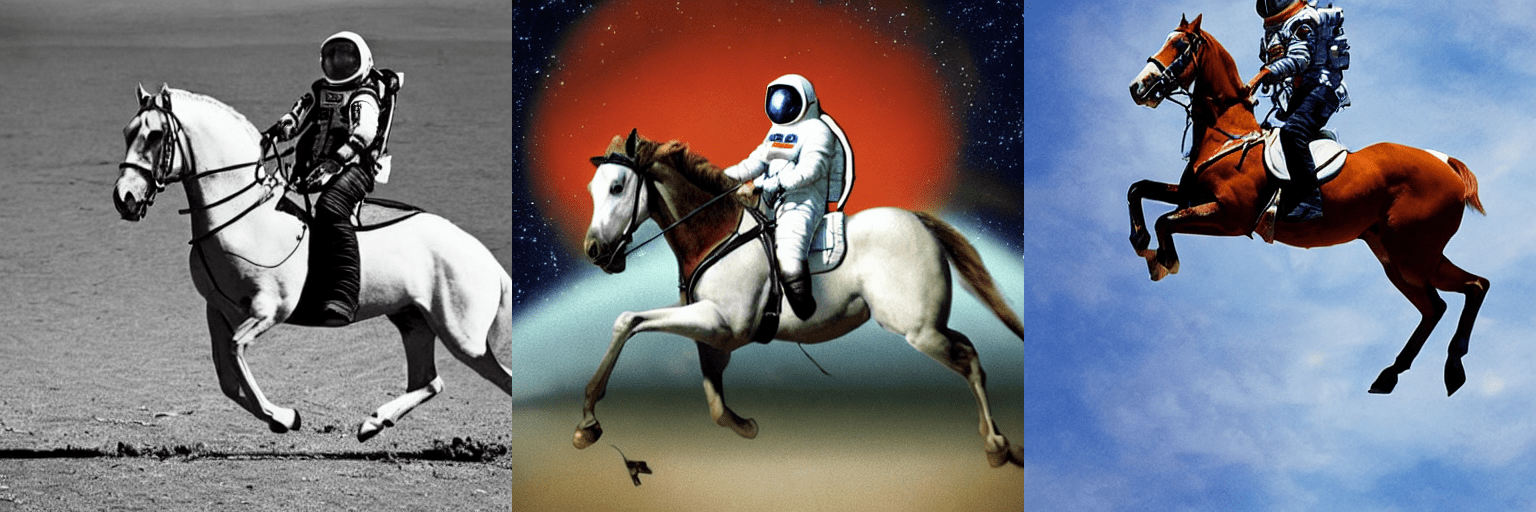
\includegraphics[width=\textwidth]{img/ai-gallery3}
    \end{columns}
\end{frame}
